\chapter{Modeling of Physics Processes} 
\label{chapter:modeling}

\section{Monte Carlo Simulation}
\subsection{Motivation} \label{subsection:simulation}

An accurate modeling of the physics processes occurring in collisions is needed in order to search for a specific signal process in the experimental data. The physics of pp collisions is modeled numerically based on existing theoretical predictions by solving complex integrals and equations over a multidimensional space of involved particles, kinematic properties, and theoretical parameters. For modeling purposes, their analytical or numerical evaluation is impractical. However, the Monte Carlo (MC) method was formally developed by John Von Neumann and Stanislaw Ulam (1940s), to study the distance that neutrons will likely travel in a material. This method is able to randomly sample predictions of important system variables, assuming they are fully described by probability density functions. Particle physicists have developed MC simulation tools to model physics processes.

%Event generators
MC event generators are used to model the physics phenomena in high-energy collisions. An example of the physics phenomena described by an event generator is seen in Figure~\ref{fig:collisionproducts}. These generators provide a description of the different regimes of the collision event: hard parton scattering, parton showering, hadron formation or hadronization, and unstable hadron decays. These tools generate events with a theoretical precision that can include higher orders in the perturbative calculations beyond “tree-level” Feynman diagrams (e.g. NLO). Some well-established tools are the matrix element and parton scattering generator MadGraph~\cite{Alwall:2014hca}, and PYTHIA~\cite{Sjostrand:2014zea} which evolves the parton-level event to the final state. 

%Geant4 or FLUKA
To search for events of interest in the experimental data, we need to know how the detector layers will respond to them and reconstructs them. This information is obtained via MC detector simulation using programs such as GEANT4~\cite{Agostinelli:2002hh} or FLUKA~\cite{Ferrari:2005zk}. The general procedure is to implement a detailed detector model (geometry, materials, alignment, etc.). Then, the program models the propagation of the event generated particles through the detector layers and their interaction with the materials. The detector interactions are translated into realistic signals (digitization) as well, and then the same event reconstruction used in real data is applied.

\clearpage

\begin{figure}[htbp!]
\centering
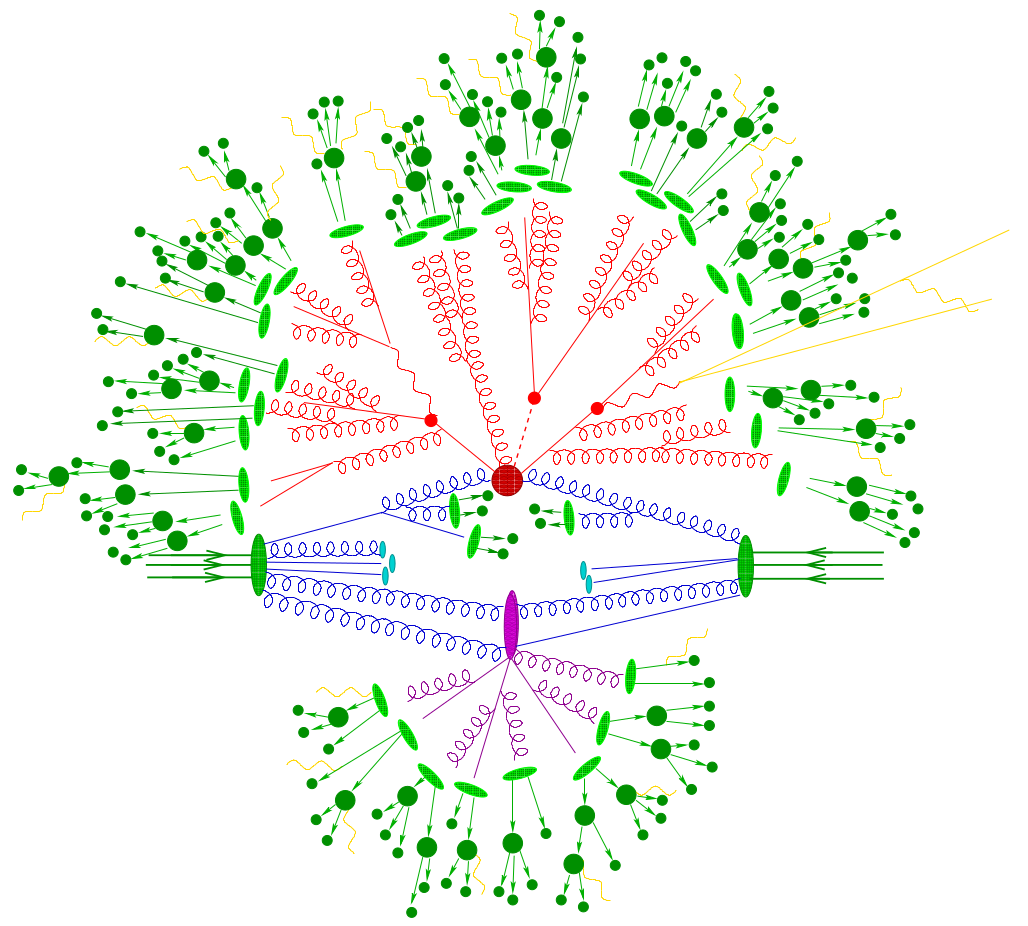
\includegraphics[width=0.85\linewidth]{Figures/Modeling/Signal/collision.png}
\caption[Sketch of processes involved in a proton-proton collision]{Sketch of processes involved in a proton-proton collision~\cite{Gleisberg:2008ta}. The hard scattering process (big red circle) corresponds to the production of a Higgs boson in association with two top-quarks or $\ttbarh$ (three small red circles). The secondary interaction or underlying event (big purple ellipse) is also shown. Before hadron formation (green light ellipses), parton showering and radiation takes place (red). Hadron decays (dark green circles) and photon emission (yellow) are shown as well.}
\label{fig:collisionproducts}
\end{figure}

\subsection{Simulated Samples}
%Simulated samples
The production of signal and backgrounds processes in pp collisions are simulated using Monte Carlo (MC) simulations. The full simulation is carried out independently per year or `campaign', considering the detector and data-taking conditions (i.e. PU profile and luminosity). 

For ggF anomalous coupling modeling, signals with $\kl=0,~1,~2,~2.45,~5$ are simulated at NLO precision in QCD using the POWHEG generator~\cite{Alioli:2008gx, Nason:2004rx, Frixione:2007vw} with the NNPDF3 parton distribution function set at the NNLO precision. For VBF anomalous coupling modeling, signals with seven different combination of $(\kv, \kvv, \kl)$ couplings are generated at LO precision using the MadGraph5\_aMC@NLO generator. In addition, ggF signals are simulated at LO accuracy in the MadGraph5\_aMC@NLO generator, and used for BSM EFT benchmark modeling (Table~\ref{tab:eftcouplings}).

Background events are simulated to study the background event properties, but they are not used in the nominal background model. The dominant background events, QCD multijet production, are generated using MadGraph5\_aMC@NLO at LO accuracy and by regions of the scalar sum of the transverse momentum (or HT) of scattering partons at matrix element. The $\ttbar$ production is generated at NLO accuracy using the POWHEG generator and normalized to the NNLO theoretical cross section~\cite{Czakon:2011xx}. Other minor backgrounds (Single Higgs production, ZZ$\rightarrow$4b) are also simulated. The list of samples and their normalization cross sections are presented in Tables~\ref{samples:tab:MC2016}, \ref{samples:tab:MC2017} and \ref{samples:tab:MC2018}  in the Appendix~\ref{appendix:samples}.

All generated events are interfaced with PYTHIA8~\cite{Sjostrand:2014zea} for parton showering, hadronization, and decays. Additional pp collisions are superimposed on the main event to simulate the PU particle environment. Then, the CMS detector response simulation is carried out using GEANT4~\cite{Agostinelli:2002hh}. Lastly, the CMS event reconstruction is performed as if the simulated events were data. 
 
Several corrections are applied to the simulated events to better model the recorded data. Object-level corrections correspond to jet energy scale and resolution corrections, and to b-tag efficiency scale factor. An additional event-level correction is applied to the simulated events to better model the pileup distribution measured in the data. An event weight is applied and corresponds to the ratio of the normalized distributions of pileup interactions in simulation and in data. The pileup weights are normalized to a total sum of one for every sample processed, ensuring that the total normalization of each simulated process is not altered. A weight to correct for differences in the trigger efficiency between data and simulation is applied (see Section~\ref{sec:trigger}).

\subsection{HH Signal Model}
A generalized signal HH model is used to compute the total cross section and kinematic distributions as function of arbitrary values of ggF and VBF couplings.
Moreover, a dedicated ggF EFT signal model is implemented. The HH model initially developed in the context of the analysis presented here is used in all the other non-resonant HH analyses prepared or under preparation by the CMS Collaboration.

For the ggF signal, a linear combination of three NLO ggF signal samples is used to model the total and differential cross sections (i.e. kinematic variables)  for an arbitrary $\kl$ and $\kt$ coupling values. The linear combination coefficients are computed using polynomial functions of the $\kl$ and $\kt$ couplings derived from the known dependence on the production cross section. The concepts behind the method are described in Section~\ref{sec:ggfsignalmodel} of the Appendix~\ref{appendix:hhsignalmodel}. The signal yields are scaled to match the cross section at NNLO accuracy taking into account the $\kl$-dependency, as illustrated in Figure~\ref{fig:xsvbf} A). The optimal combination of ggF samples optimal is the one corresponding to $\kl$=1, 2.45 and 5 samples. 

The VBF signal modeling follows a similar approach to the one in the ggF signal modeling. However, the linear combination is carried out using six VBF simulated signals. The parametrization of the coefficients is further described in Section~\ref{sec:vbfsignalmodel} of the Appendix~\ref{appendix:hhsignalmodel}. Using the expected LO cross section dependence on the coupling values and the SM $\mathrm{N^{3}LO}$ prediction, the total signal yields are scaled to match the $\mathrm{N^{3}LO}$ accuracy. The optimal choice of signal samples is presented in Table~\ref{tab:hhsignalsamples}. The resulting VBF HH production cross section dependency on the three individual couplings is illustrated in Figure~\ref{fig:xsvbf} B-D).

\begin{table}[htb!]
\caption[Couplings variations used for the ggF and VBF signal models]{Couplings variations used for the ggF and VBF signal models. The ggF (VBF) listed values of cross section times the branching fraction, $\mathrm{\sigma(pp\rightarrow HH) \cdot B(HH\rightarrow bbbb)}$, are taken from the generator and scaled to the $\mathrm{NNLOFTapprox}$ ($\mathrm{N^{3}LO}$) precision by a factor \hbox{$\mathrm{k=\sigma_{NNLOFTapprox}^{SM} / \sigma_{generator}^{SM}=1.16}$} (\hbox{$\mathrm{k=\sigma_{N^{3}LO}^{SM}/\sigma_{generator}^{SM}=1.04}$}). }
\label{tab:hhsignalsamples} 
\centering
\begin{tabularx}{\textwidth}{lXX}
	\hline
    Model                     & Coupling values  & $\mathrm{\sigma(pp\rightarrow HH) \cdot B(HH\rightarrow bbbb)}$[pb]\\
	\hline
ggF $(\kl,\kt)$          & 1,1     & 0.010517 \\	
ggF $(\kl,\kt)$          & 2.45,1  & 0.004455 \\
ggF $(\kl,\kt)$          & 5,1     & 0.031072 \\
VBF $(\kl,\kv,\kvv)$     & 1,1,1                  & 0.000585\\	
VBF $(\kl,\kv,\kvv)$     & 1,1,0                  & 0.009169\\
VBF $(\kl,\kv,\kvv)$     & 1,1,2                  & 0.004823\\
VBF $(\kl,\kv,\kvv)$     & 2,1,1                  & 0.000482\\
VBF $(\kl,\kv,\kvv)$     & 0,1,1                  & 0.001558\\
VBF $(\kl,\kv,\kvv)$     & 1.1.5,1                & 0.022412\\
	\hline
\end{tabularx}

\end{table}

\clearpage
An EFT ggF signal model is used to simulate the 12 benchmarks presented in Table~\ref{tab:eftcouplings} at NLO precision. First,  each benchmark signal follows the recipe of the ggF LO modeling detailed in Section~\ref{sec:ggfsignalmodel} in Appendix~\ref{appendix:hhsignalmodel}. Then, a reweighting procedure is applied to these events, in order to correct the $\hhm$ spectrum from LO to NLO accuracy in QCD following Ref.~\cite{Buchalla:2018yce}. 

\begin{figure}[htbp!]
\centering
\captionsetup[subfigure]{justification=centering}
\subfloat[]{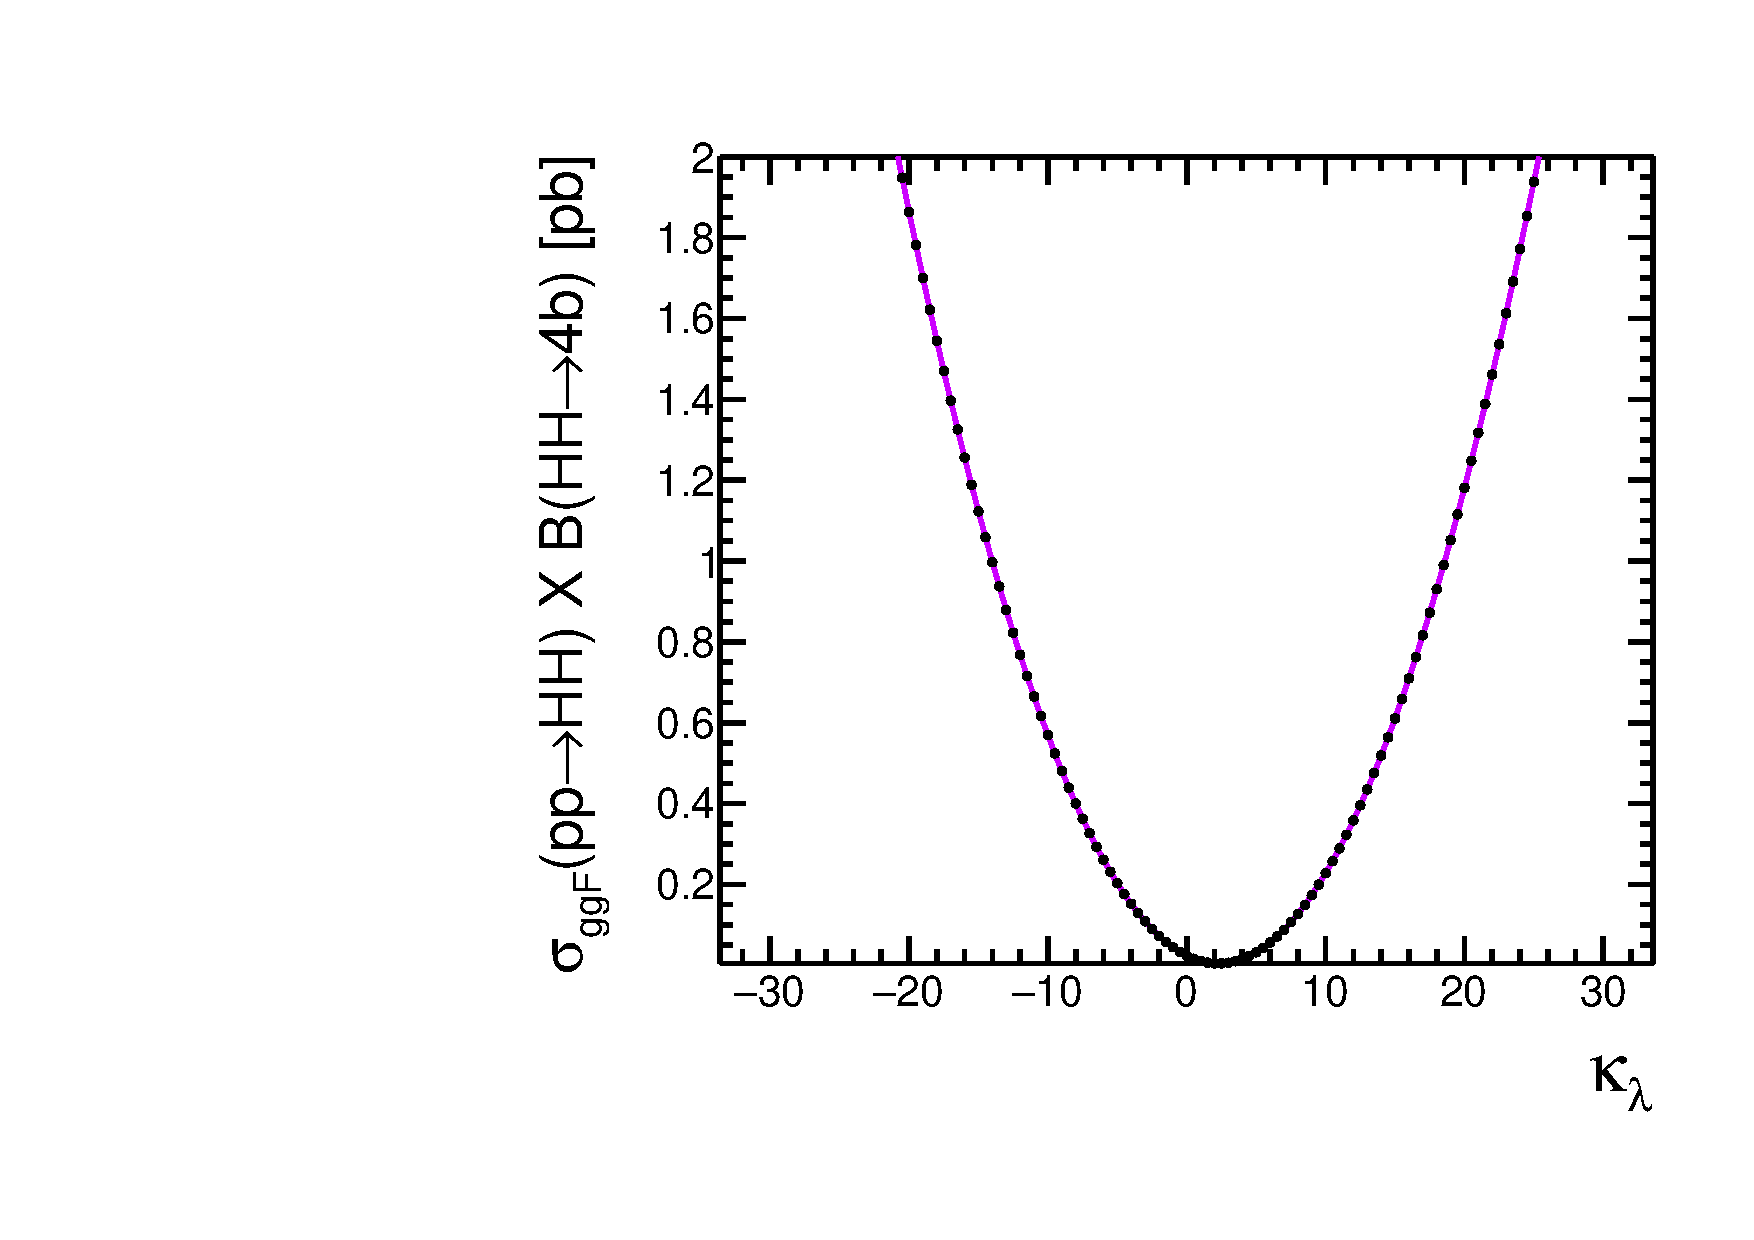
\includegraphics[width=0.48\linewidth]{Figures/Modeling/Signal/kl_line.pdf}}
\subfloat[]{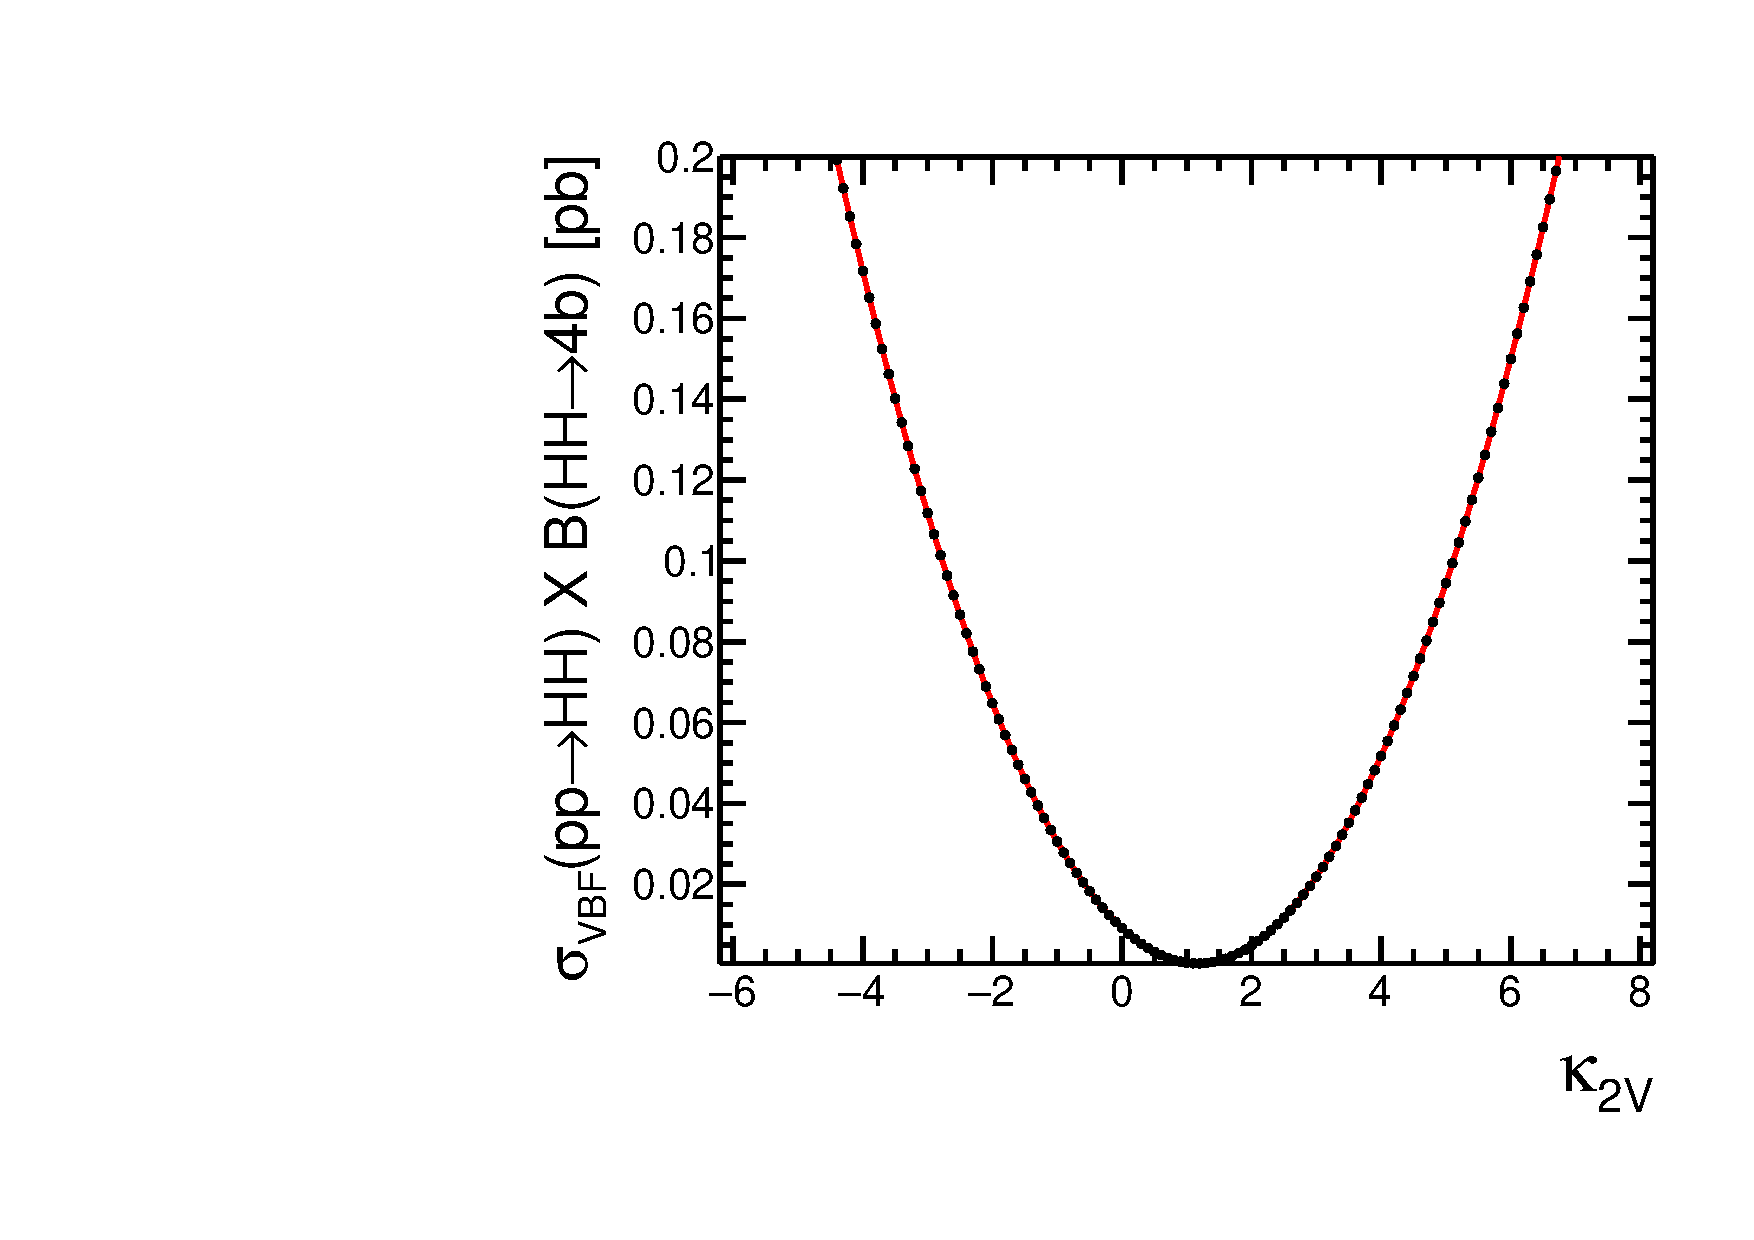
\includegraphics[width=0.48\linewidth]{Figures/Modeling/Signal/k2vline.pdf}}\\
\subfloat[]{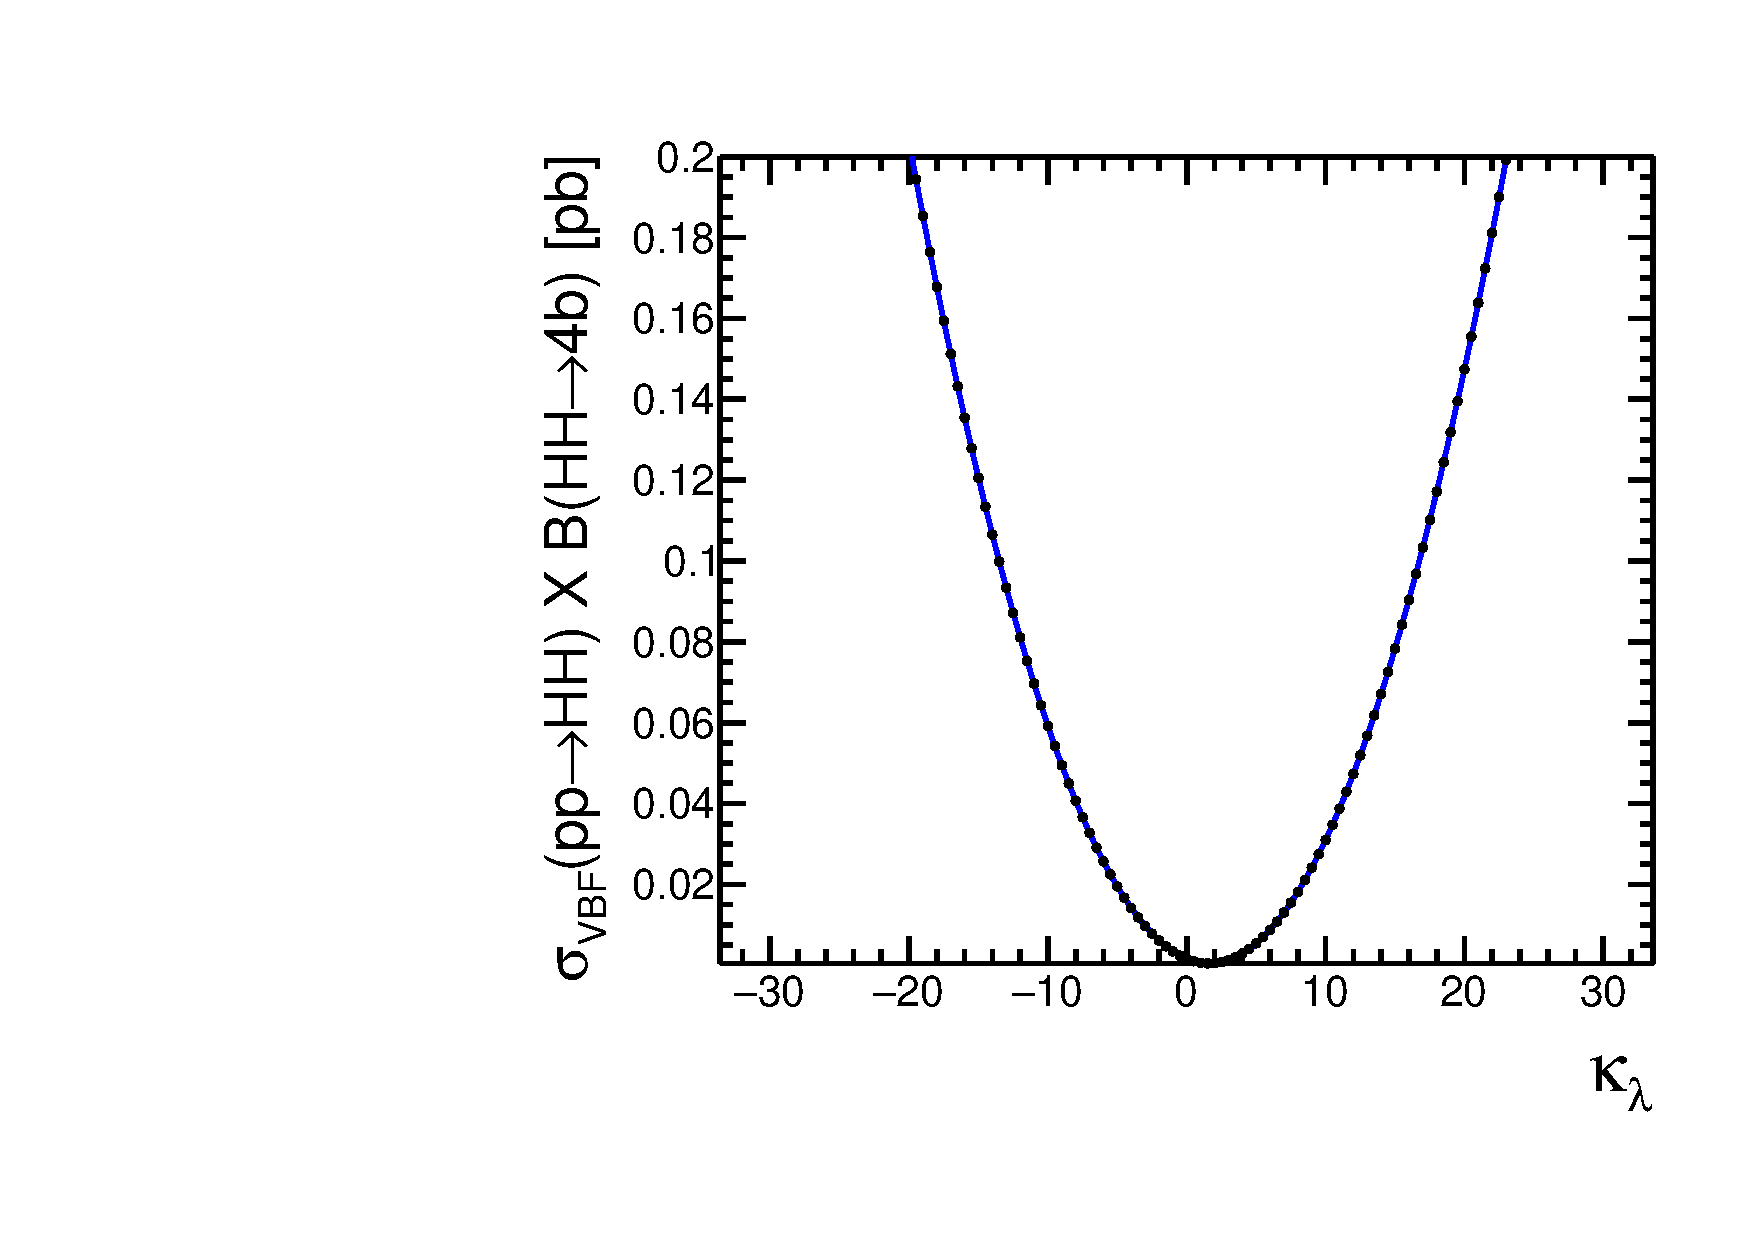
\includegraphics[width=0.48\linewidth]{Figures/Modeling/Signal/k3line.pdf}}
\subfloat[]{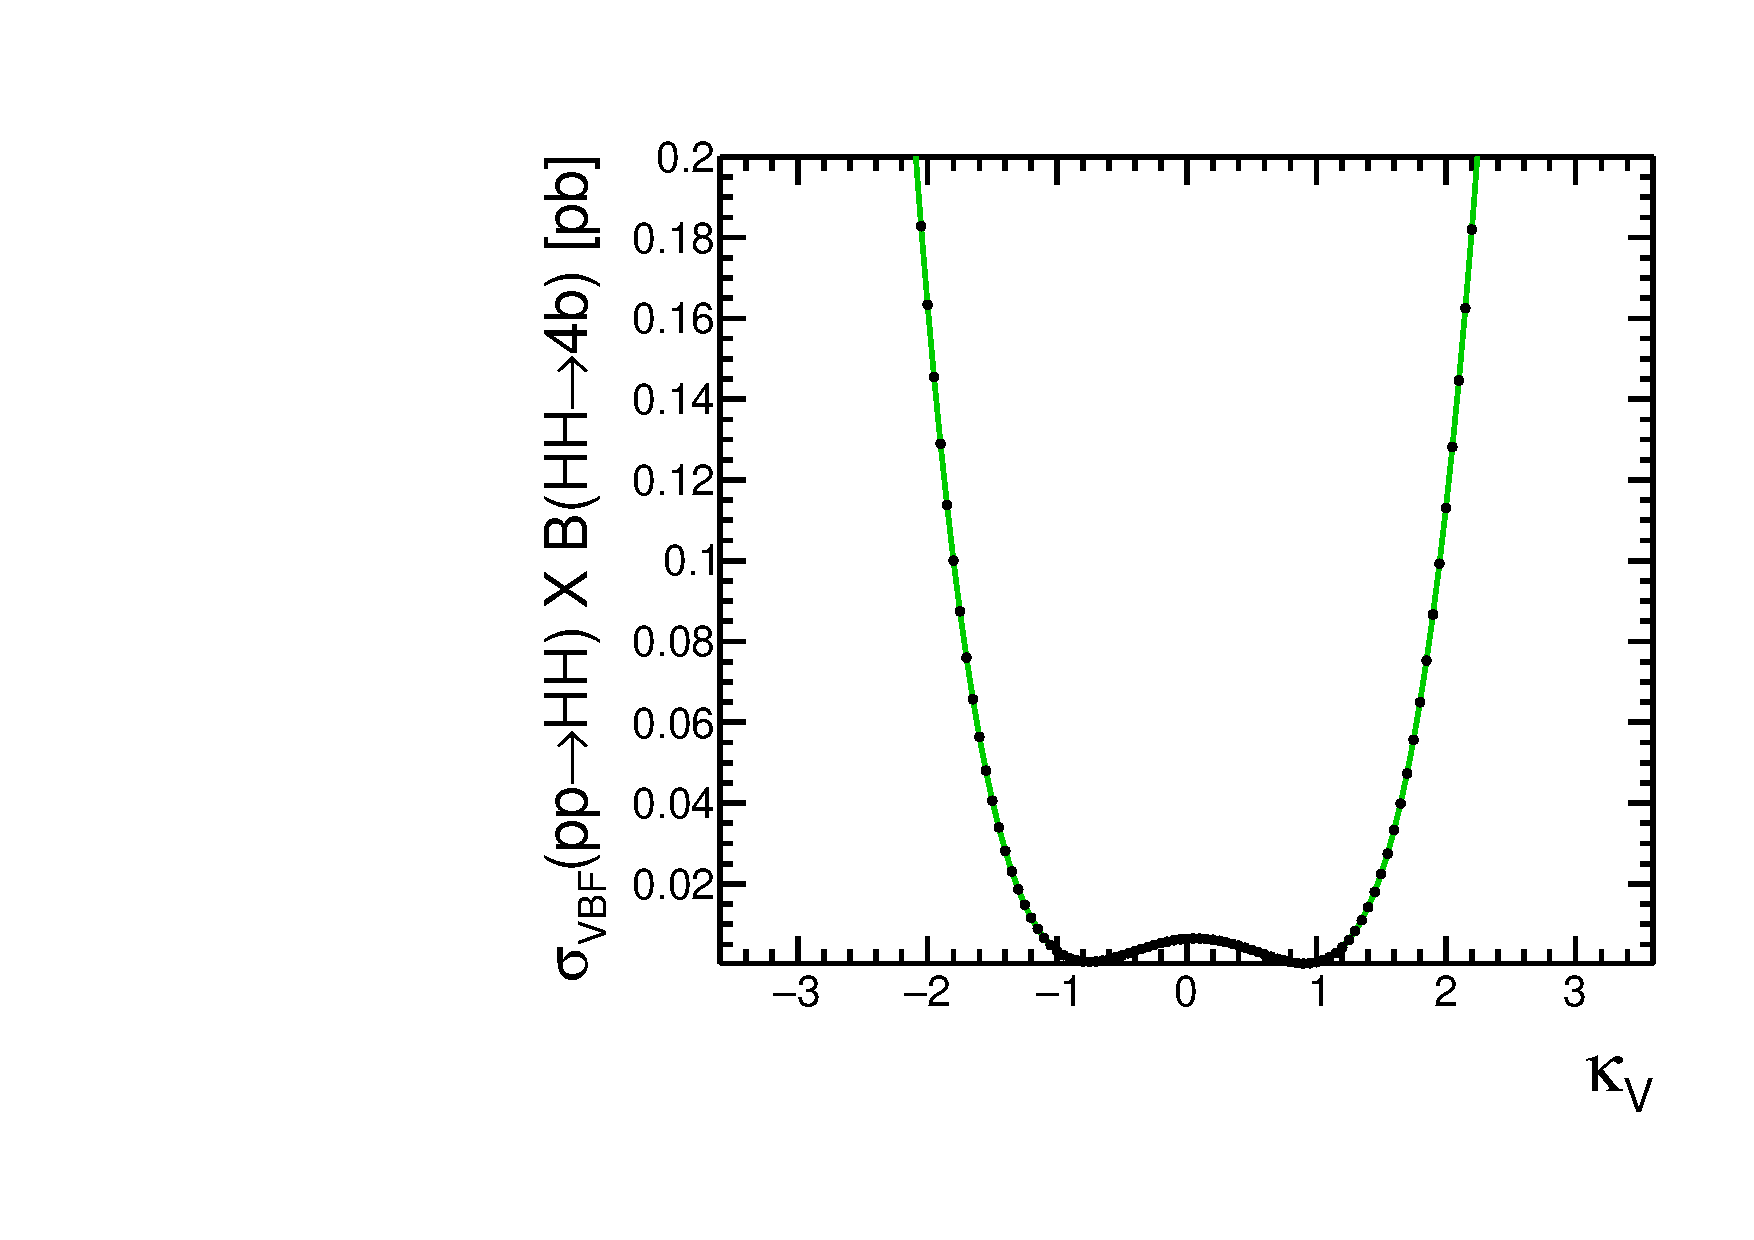
\includegraphics[width=0.48\linewidth]{Figures/Modeling/Signal/kvline.pdf}}
\caption[Higgs boson pair production cross section times the branching fraction into four bottom quarks as a function of the couplings using the signal modeling]{Higgs boson pair production cross section times the branching fraction into four bottom quarks as a function of the couplings using the signal modeling. A) ggF mode vs $\kl$, B) VBF mode vs $\kvv$, C) VBF mode vs $\kl$,  D) VBF mode vs $\kv$.}
\label{fig:xsvbf}
\end{figure}

\section{Data-driven Background Model}
\label{sec:backgroundmodel}
\subsection{Motivation}
In LHC searches for $\mathrm{HH\rightarrow~bbbb}$, the dominant QCD multijet background events are not properly modeled by MC simulation. Consequently, a background model is typically derived using real collision data events. These kinds of methods are known as a `data-driven' methods.

In the published CMS 2016 data-only version of this search~\cite{bbbbcmsnr}, the background model strategy used a data-driven method. An artificial ensemble of background events (QCD, $\ttbar$ and others) are produced by mixing event hemispheres from real `4b' data events using a method called the `Hemisphere-mixing'. This technique has a good modeling when tested in QCD MC events. However, when applied to the data (containing other minor backgrounds), a systematic bias on the background shape is observed. The background shape and normalization uncertainties can affect the analysis sensitivity by ~30 and ~9\%, respectively. 

The published ATLAS 2015-2016 data-only analysis uses a background model that combines a QCD multijet data-driven estimation and $\mathrm{t\overline{t}}$ simulation~\cite{bbbbatlas}. The ATLAS data-driven multijet model part takes events from a `2b' region to model `4b' region events. There are kinematic differences between the two datasets, which are corrected with event-by-event correction weights or reweighting procedure. The weights are derived using an iterative method involving several 1D histograms. This method performs well within the uncertainties. However, being an iterative method based on 1D reweightings, it is hard to use it to model a multivariate discriminant that we can use to boost the signal separation from the background.

The background model presented in this dissertation is developed for the Run-2 result, replacing the one in the previous CMS 2016-only result. It uses a machine learning algorithm proposed to solve the problem of simultaneously reweighting of multiple distributions called the `Boosted Decision Tree reweighting' or BDT reweighting from here~\cite{Rogozhnikov:2016bdp}. It is the first time that is this method is applied in a CMS analysis. It has been applied in ATLAS~\cite{ATLAS:2018tti,ATLAS:2020qiz} and LHCb searches~\cite{LHCb:2016jrk} in the past. The machine learning algorithm is described in Subsection~\ref{subsec:bdtr}, and its implementation in the data analysis is presented in Subsection~\ref{subsec:imp}.

\subsection{Boosted Decision Tree Reweighting} \label{subsec:bdtr}

In high energy physics is very common to study a `base' dataset (e.g. MC simulated events) with discrepancies and imperfections among multiple variables with respect to a `target' dataset (e.g. collected data). A reweighting procedure is commonly introduced to improve the variables' agreement. Mathematically, a reweighting problem between two datasets is equivalent to find the density ratio function $\rho\mathrm{(x)=f_{target}(x)/f_{base}(x)}$, where x corresponds to an N-dimensional vector of the variables involved in the reweighting.

One approach to determine $\rho(x)$ is the `Reweighting with bins' method. In this method, the multivariable phase space is split into $k$ bins, and then each bin of base events are multiplied by a factor $\alpha\mathrm{_{k}= \frac{w_{k,target}}{w_{k,base}}}$, where $\mathrm{w_{k,base}}$ and $\mathrm{w_{k,target}}$ correspond to the total weight of events in the bin-$\kappa$ in the base and target dataset. In practice, the ratio of histograms representing the densities of events in this space. However, although the technique is very intuitive and simple, it has the following limitations: 
\begin{itemize}
    \item Only a few variables can be reweighted simultaneously with good performance
    \item Choosing what variables to re-weight is not simple as one variable often brings disagreement to others
    \item It can give an unstable reweighting rule for bins of the input density histograms that are scarcely populated because of the large statistical fluctuations
\end{itemize}

A machine learning algorithm to solve this exact problem is proposed in Ref.~\cite{Rogozhnikov:2016bdp}. In this algorithm, a decision tree is used to split the phase space into two regions (or leafs of the tree) with the largest event weight difference, i.e. find the regions that require more reweighting. To that end, the metric in equation~\ref{eq:chi2} is maximized, where $\mathrm{w_{leaf,base}}$ and $\mathrm{w_{leaf,target}}$ correspond to the total weight of events in the leaf of the base and target dataset.
\begin{equation}\label{eq:chi2}
\chi^{2} =  \sum_{ \mathrm{leaf}  }  \mathrm{ \frac{(w_{leaf,base} - w_{leaf,target})^{2} }{ w_{leaf,base} + w_{leaf,target} }   }  
\end{equation}

The BDT reweighter consists of a forest of N trees, each trained one by one with these steps:
\begin{enumerate}
\item Build the decision tree that maximizes the $\chi^{2}$ function. It determines the cut that maximizes the $\chi^{2}$ function for each variable. Then, the sample is sliced into two using the variable with maximal $\chi^{2}$. For each resulting slice, the same procedure is repeated until defined criteria (maximum depth, minimum events in the leaf, etc.) is satisfied.  
\item Compute the weight in a given leaf as $\mu\mathrm{_{leaf}= \log \left(\frac{ w_{leaf,base} }{ w_{leaf,target} }\right)  }$
\item Before training a new tree, the current tree weights are applied to the base sample as $\mathrm{w_{tree}=}\exp(\lambda\mu\mathrm{_{leaf}})$, where $\lambda$ is the learning rate.  
\end{enumerate}

In the last step, the event-by-event weight is determined as the product of the contributions from the individual trees  (i.e. boosting), $\mathrm{w=\displaystyle \prod_{i=1}^{ \mathrm{N} } w_{i}}$. By following this procedure, the BDT reweighter captures the differences between the base and the target datasets, taking into consideration multiple variables and their correlations. This method is expected to have better performance than algorithms such as bin-reweighting, re-used general-purpose classification scores based on boosted decision trees (BDTs) or artificial neural networks  (ANNs).

\subsection{Implementation} \label{subsec:imp}
\subsubsection{Overview} \label{subsub:bkgoverview}

The derivation of the data-driven background model begins selecting real data events from a high statistics region orthogonal to the `4b' real data. As seen in Subsection~\ref{sec:btagregions}, the `3b' region has around 7-10 times more data events than the `4b' region. In consequence, events from this region are chosen as the `base' dataset to model the background in the `target' 4b region. If CMS had a `2b' trigger during the data-taking, we could exploit data from an additional 2b region for the background modeling. 

The 3b and 4b data events are expected to differ in event yields and kinematic properties. The latter is due to differences in b-tagging efficiency and jet activity, among other effects. Furthermore, a multivariate model is needed to accurately and simultaneously model the input variables of the MVAs used in the ggF categories (described in Subsection~\ref{subsec:ggfvbfobservales}). Consequently, a multidimensional transfer model is built to transfer the event yield and event distributions from the 3b region to the 4b region. To this end, the analysis signal ($\mathrm{A_{SR}}$) region and analysis control ($\mathrm{A_{CR}}$) region defined in Subsection~\ref{sec:analysisregions} are note. Note that $\mathrm{A_{SR}}$(4b) is the target region for the search because it has the best signal-to-background ratio. The $\mathrm{A_{SR}}$(4b) background model is derived using information from the $\mathrm{A_{CR}}$(3b), $\mathrm{A_{CR}}$(4b) and $\mathrm{A_{SR}}$(3b) regions. 

The multidimensional transfer model is prepared using $\mathrm{A_{CR}}$ data events and then is applied to the $\mathrm{A_{SR}}$(3b) events to derive the $\mathrm{A_{SR}}$(4b) background estimate. It addresses the background shape and events yields separately. The background normalization is imposed in the background model template. It is computed correcting the $\mathrm{A_{SR}}$(3b) normalization, taking into consideration the yield differences seen in $\mathrm{A_{CR}}$(3b) and $\mathrm{A_{CR}}$(4b) data. For this purpose, a 3b-to-4b normalization transfer factor ($\alpha$) is derived. It can be a constant or a function of a sensitive variable. The shape component corrects any residual differences between 3b and 4b data on important analysis variables. To this end, a BDT reweighter is trained to learn the differences between $\mathrm{A_{CR}}$(3b) and $\mathrm{A_{CR}}$(4b) data events. It provides a reweighting function to reshape the variables from $\mathrm{A_{SR}}$(3b) events to better model $\mathrm{A_{SR}}$(4b) ones.

The background model method is fully validated in a separate region, where both the validation signal ($\mathrm{V_{SR}}$) and control ($\mathrm{V_{CR}}$) regions are redefined to be incompatible with the SM $\hm$ mass hypothesis. The requirements of the validation region are presented in Subsection~\ref{sec:analysisregions}. The validation tests are detailed in Subsection~\ref{sec:bkgvalidation}. Moreover, extra tests in Subsection~\ref{sec:additionalchecks} check the impact of SM HH signal and single Higgs production contamination in the modeling.  

Each event subcategory has its own $\mathrm{A_{SR}}$(4b) background estimate. Note that as the VBF category 2 signal extraction is defined as a single counting-experiment (see more in Chapter~\ref{chapter:results}), no shape correction is needed. To avoid any bias on the background model, the $\mathrm{A_{SR}}$(4b) region data are `blinded' until the method is finalized, reviewed, and the data unblinding is approved by CMS.

\subsubsection{Background normalization} \label{sec:bkgnorm}
The normalization transfer factor $\alpha$ can be calculated by taking the ratio of number of events in the $\mathrm{A_{CR}}$(4b) and $\mathrm{A_{CR}}$(3b) regions. Then, it is applied to the $\mathrm{A_{SR}}$(3b) normalization to predict the $\mathrm{A_{SR}}$(4b) background normalization using the following equation: \begin{equation}\label{eq:tfconstant}
\mathrm{N(A_{SR}^{4b})_{\alpha} =\frac{ N(A_{CR}^{4b}) }{ N(A_{CR}^{3b}) } \cdot N(A_{SR}^{3b})  = \alpha \cdot N(A_{SR}^{3b}) }
\end{equation}

The previous method assumes that $\alpha$ is a constant across the ($\hfstm,\hsndm$) plane. Within the $(\hfstm, \hsndm)$ plane, events are naturally described by two quantities defined by the projections of each point of the plane along the axes parallel and perpendicular to the diagonal used for the reconstruction of the two $\hfstm$ candidates ($\hfstm = 1.04 \times \hsndm$). We refer to these two quantities as the ``parallel`` and ``perpendicular`` masses, and denote them with $\mathrm{m_{paral}}$ and $\mathrm{m_{perp}}$, respectively. Events have a similar kinematics as function of $\mathrm{m_{perp}}$, since an increase in the mass of $\hfstm$ is compensated by a reduction of the mass of $\hsndm$. Inversely, smaller and larger values of $\mathrm{m_{paral}}$ correlate with softer and harder event kinematics, impacting the value of the $\alpha$ transfer factor. Since the number of events in the 3b region is not flat as a function of $\mathrm{m_{paral}}$, this can bias the determination of the background normalization. The effect magnitude is illustrated in Fig.~\ref{fig:bkg:mdep_SF}.  

\begin{figure}[htbp!]
\captionsetup[subfigure]{justification=centering}
\begin{center}
\subfloat[]{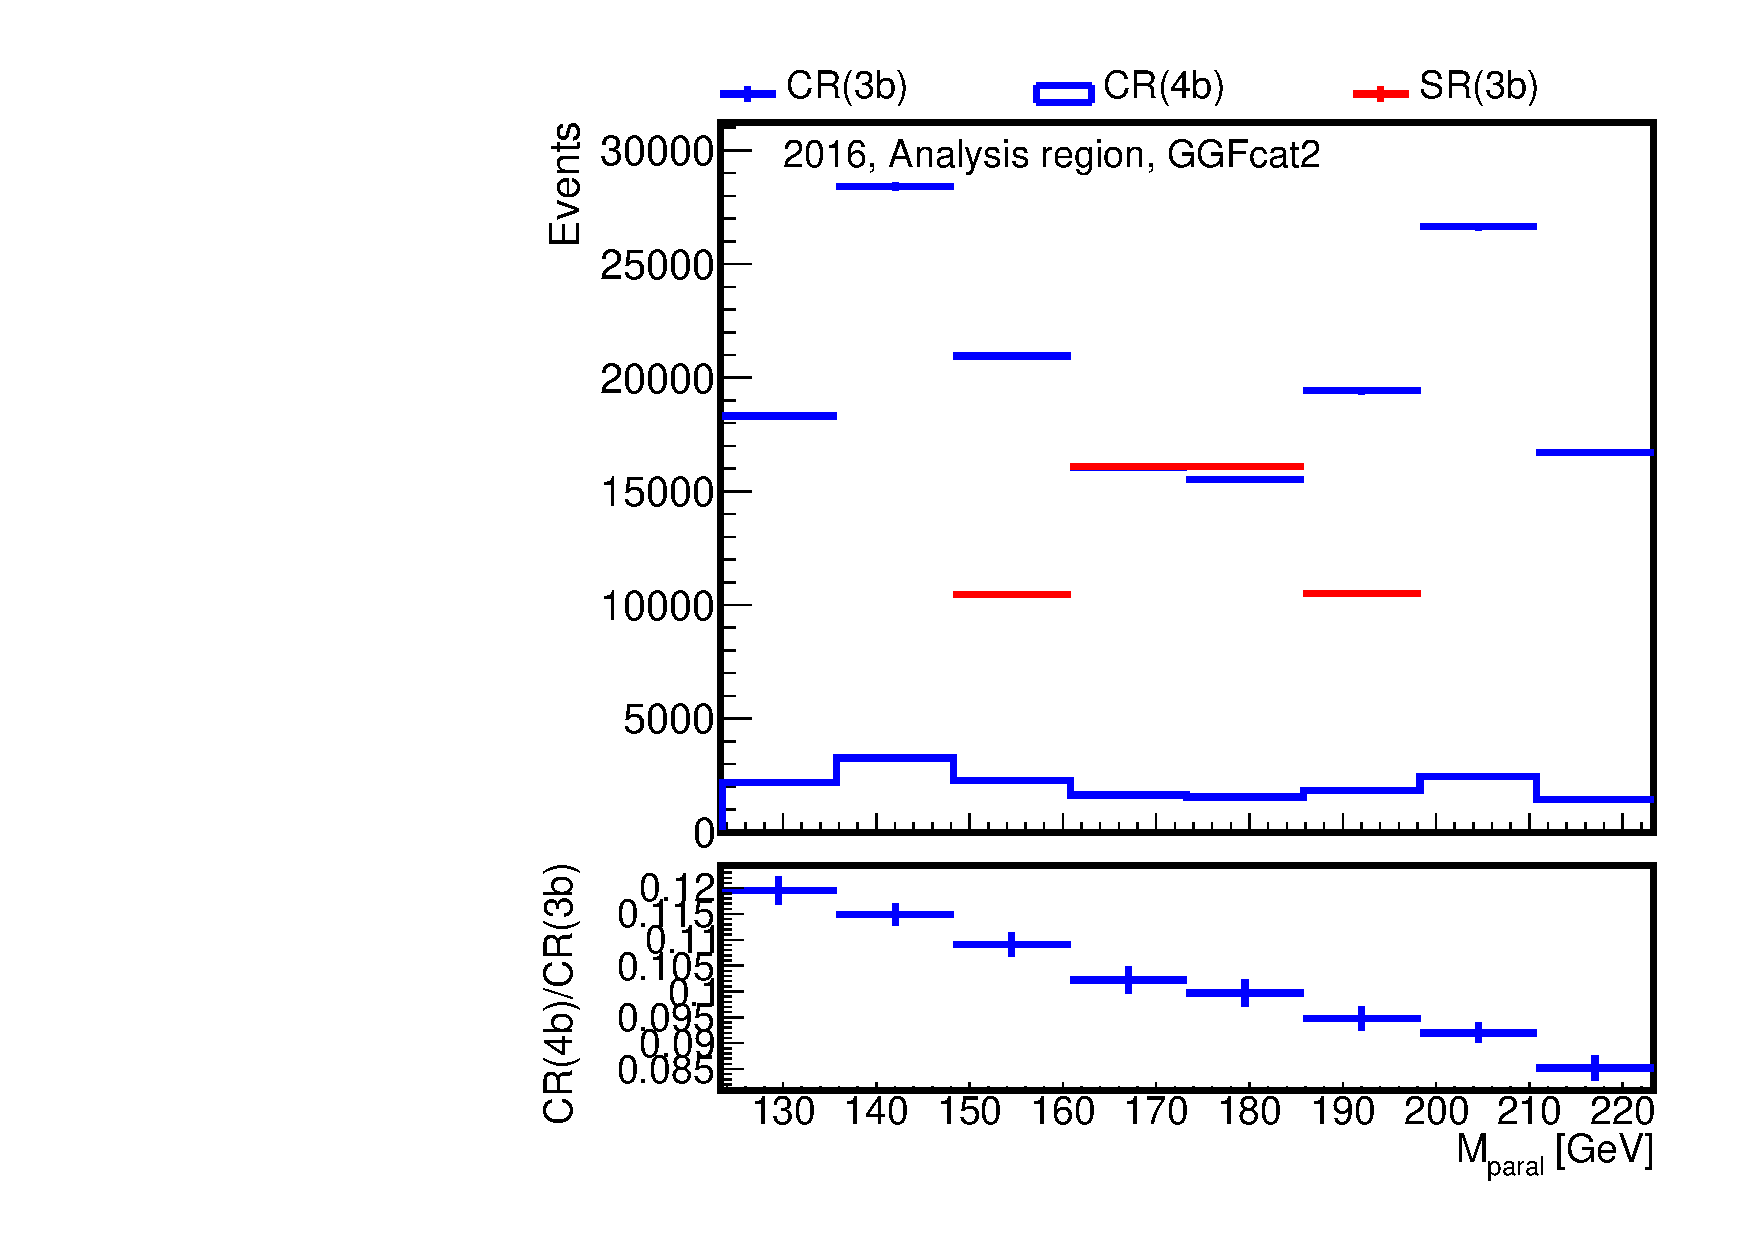
\includegraphics[width=0.50\linewidth]{Figures/Modeling/background/mdepTF/comparison_2016NonResonantAnalysis_Weight_AnaGGF2.pdf}}
\subfloat[]{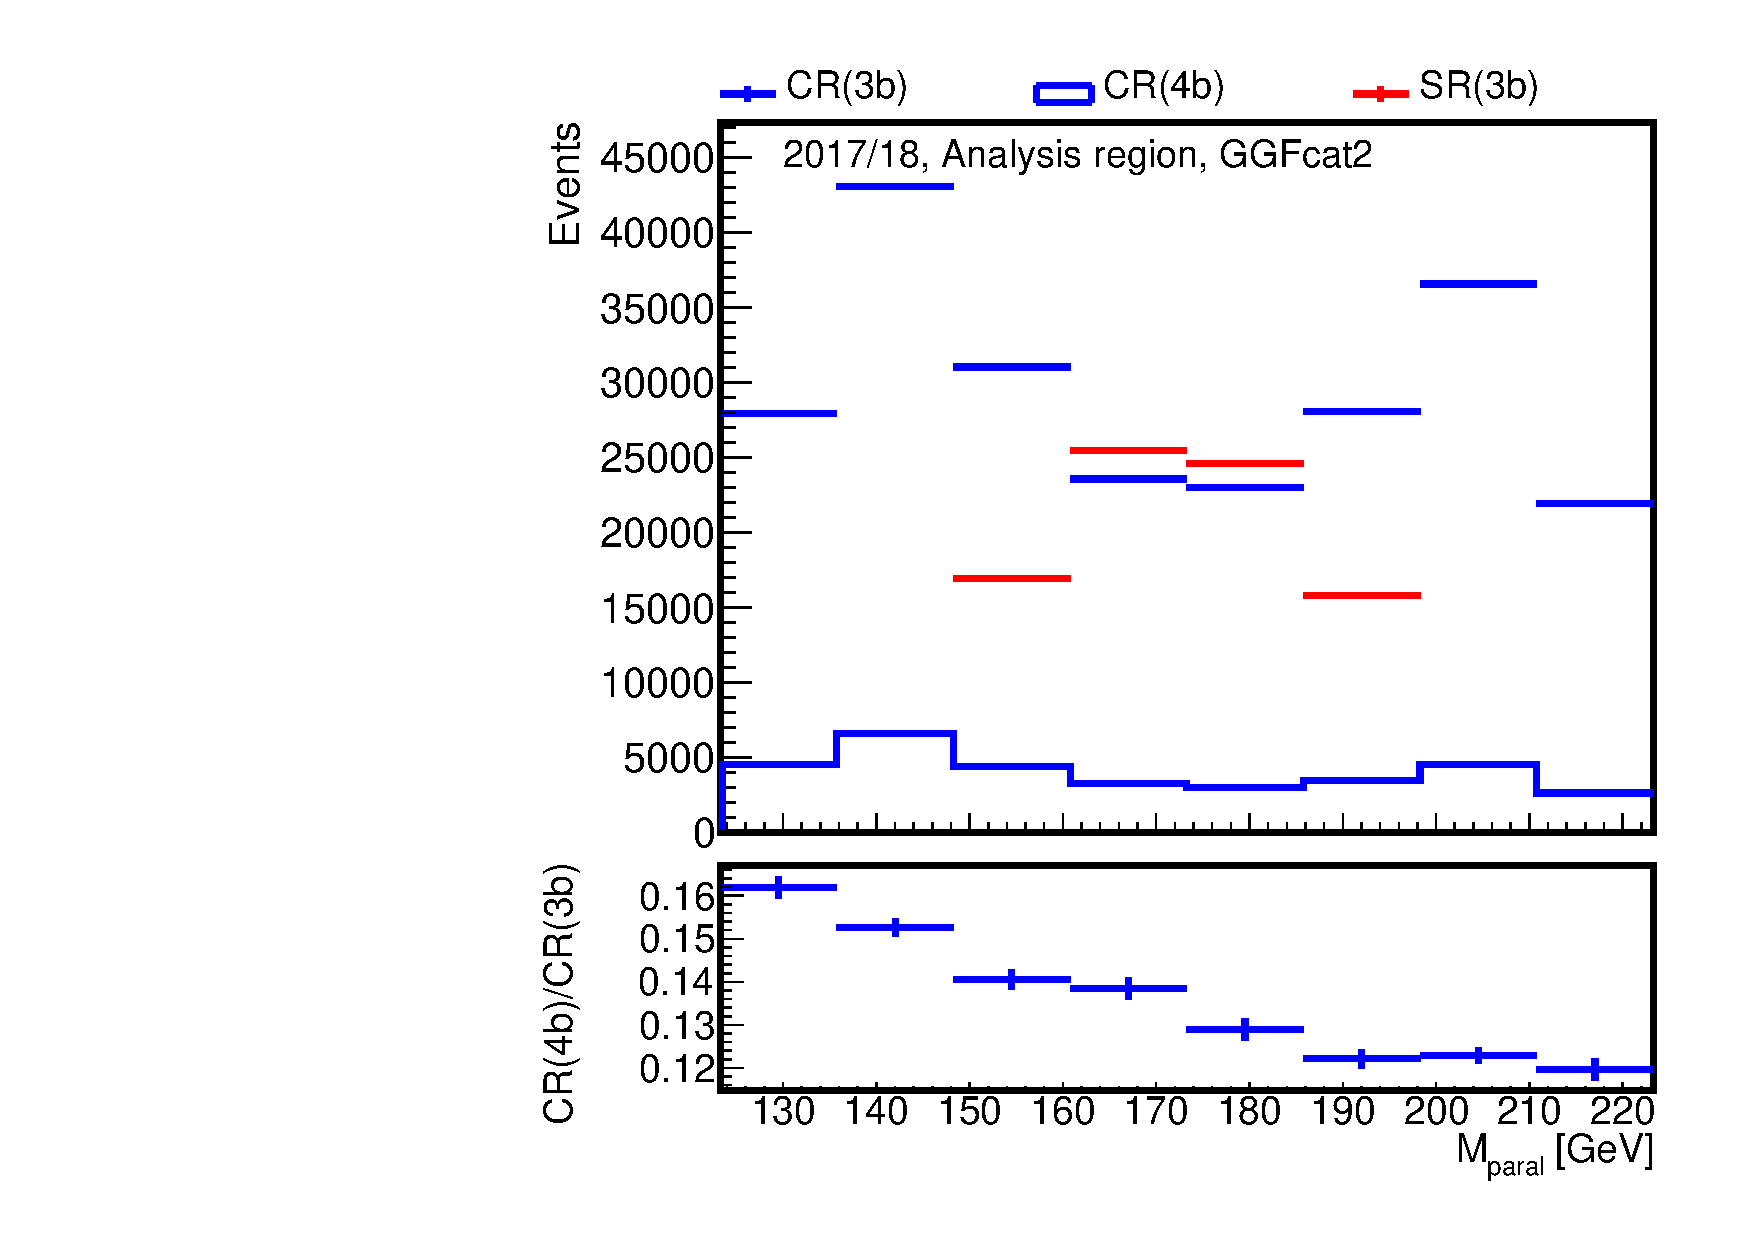
\includegraphics[width=0.50\linewidth]{Figures/Modeling/background/mdepTF/comparison_20172018NonResonantAnalysis_Weight_AnaGGF2.pdf}}
\end{center}
\caption[Dependence of the normalization transfer factor on the $\mathrm{m_{\parallel}}$ variable]{Dependence of the normalization transfer factor on the $\mathrm{m_{\parallel}}$ variable, illustrated for the ggF category 2 in A) 2016 data and B) 2017-2018 data.}
\label{fig:bkg:mdep_SF}
\end{figure}

For ggF subcategories, the adopted strategy is to first divide the CR data in eight bins of $m_{\parallel}$, and compute the value of $\alpha$ in each of them. Then, this dependency is used on $\mathrm{A_{SR}}$(3b) events to derive an alternative estimation of the SR(4b) normalization following equation~\ref{eq:tfnoconstant}. For VBF subcategories, however, the number of events is too small and possible trends are covered by the statistical fluctuations of data and by their associated uncertainties. Consequently, for this case, the strategy is to apply the constant transfer factor following equation~\ref{eq:tfconstant}. 
\begin{equation}\label{eq:tfnoconstant}
\mathrm{N(A_{SR}^{4b})_{\alpha,\parallel} = \sum_{ibin}  \left(\frac{ N(A_{CR}^{4b}) }{ N(A_{CR}^{3b}) }\right)_{ibin} \cdot  \left(~N(A_{SR}^{3b})~\right)_{ibin}  = \sum_{ibin} (\alpha)_{ibin}  \cdot  (~N(A_{SR}^{3b})~)_{ibin}   }
\end{equation}

In Tables~\ref{bkg:tab:factor1} and \ref{bkg:tab:factor2} are shown the values of the SR(4b) background normalization predictions $\mathrm{N(A_{SR}^{4b})_{pred}}$ in all categories for the 2016 and 2017-2018 analyses, respectively. Note that there are two background normalization uncertainty sources of statistical nature: the one associated to the SR(3b) data statistical power, and the one associated to the CR statistical power.

\begin{table}[htb!]
\caption[Summary of the quantities involved in the estimation of the background normalization in the 2016 data analysis.]{\label{bkg:tab:factor1} Summary of the quantities involved in the estimation of the background normalization in the 2016 data analysis. The prediction used in the background model is denoted as $\mathrm{N(A_{SR}^{4b})_{pred}}$.}
\centering
\small
\begin{tabularx}{\textwidth}{l r r r r}
    \hline
    Subcategory                    & ggF Cat1                      & ggF Cat2                    & VBF Cat1                     & VBF Cat2                  \\
    \hline
    $\mathrm{N(A_{CR}^{3b})}$         & 94464$\pm$307.3          & 162022$\pm$402.5        & 7823$\pm$88.4            &    103$\pm$10.1       \\
    $\mathrm{N(A_{SR}^{3b})}$         & 34594$\pm$186.0          &  53129$\pm$230.5        & 2991$\pm$54.7            &     38$\pm$ 6.2       \\
    $\mathrm{N(A_{CR}^{4b})}$         &  9860$\pm$ 99.3          &  16643$\pm$129.0        & 1151$\pm$33.9            &     11$\pm$ 3.3       \\
    $\alpha$                                    & 0.10437$\pm$0.00110      &0.10272$\pm$0.00084      &0.14713$\pm$0.0046        &0.10680$\pm$0.03388    \\
    $\mathrm{N(A_{SR}^{4b})_{\alpha}}$          & 3610.9 $\pm$24.8$\pm$38.1& 5457.4$\pm$30.5$\pm$44.6     & 440.1 $\pm$8.9$\pm$13.8  &    4.1$\pm$0.7$\pm$1.3\\
    $\mathrm{N(A_{SR}^{4b})_{\alpha,\parallel}}$& 3394.8 $\pm$23.3$\pm$59.5& 5384.5$\pm$30.1$\pm$69.8     &          -               &         -             \\
    $\mathrm{N(A_{SR}^{4b})_{pred}}$            & 3394.8 $\pm$23.3$\pm$59.5& 5384.5$\pm$30.1$\pm$69.8     & 440.1 $\pm$8.9$\pm$13.8  &    4.1$\pm$0.7$\pm$1.3\\  
    \hline
\end{tabularx}
\end{table}

\begin{table}[htb!]
\caption[Summary of the quantities involved in the estimation of the background normalization in the 2017-2018 data analysis]{\label{bkg:tab:factor2} Summary of the quantities involved in the estimation of the background normalization in the 2017-2018 data analysis. The normalization used in the background model is denoted as $\mathrm{N(A_{SR}^{4b})_{pred}}$.}
\centering
\small
\begin{tabularx}{\textwidth}{l r r r r}
    \hline
    Subcategory                    & ggF Cat1                 & ggF Cat2                & ggF Cat1                  & ggF Cat2              \\
    \hline
    $\mathrm{N(A_{CR}^{3b})}$      & 101819$\pm$319.1         & 235074$\pm$484.8        & 13533$\pm$116.3           &    233$\pm$15.3       \\
    $\mathrm{N(A_{SR}^{3b})}$      &  38802$\pm$197.0         &  82715$\pm$287.6        &  5162$\pm$ 71.8           &    119$\pm$10.9       \\
    $\mathrm{N(A_{CR}^{4b})}$      &  15787$\pm$125.6         &  32222$\pm$179.5        &  2540$\pm$ 50.4           &     37$\pm$6.1        \\
    $\alpha$          & 0.15505$\pm$0.00133      &0.13707$\pm$0.00081      &0.18768$\pm$0.00406        &0.15880$\pm$0.02810    \\
    $\mathrm{N(A_{SR}^{4b})_{\alpha}}$          &  6016.2$\pm$37.5$\pm$51.6&11337.9$\pm$49.6$\pm$67.0  &  968.9$\pm$14.7$\pm$21.0  &   18.9$\pm$1.7$\pm$3.3\\
    $\mathrm{N(A_{SR}^{4b})_{\alpha,\parallel}}$&  5748.6$\pm$35.8$\pm$81.4&10998.2$\pm$48.2$\pm$104.2 &  -  & - \\
    $\mathrm{N(A_{SR}^{4b})_{pred}}$             &  5748.6$\pm$35.8$\pm$81.4&10998.2$\pm$48.2$\pm$104.2 &  968.9$\pm$14.7$\pm$21.0  &   18.9$\pm$1.7$\pm$3.3\\   
    \hline
\end{tabularx}
\end{table}

\subsubsection{Background shape} \label{sec:bkgreshape}

The background normalization procedure presented in Subsection~\ref{sec:bkgnorm} addresses the normalization of the SR(4b) background estimate. However, as explained in Subsection~\ref{subsub:bkgoverview}, there are residual differences between the `3b' and `4b' data that need to be corrected in the SR(3b) distributions to have an accurate description of the important variables of the analysis. They are corrected through a re-shaping or reweighting procedure using event-by-event weights obtained from a BDT reweighter.

The implementation of the BDT-reweighting method available in the $hep\_ml$ toolkit. The BDT reweighter is a multidimensional re-weighting rule, which training configuration is very similar to the one of any general-purpose BDT score. Therefore, the definition of the datasets, input variables, and hyperparameters is needed. The $\mathrm{A_{CR}}$(3b) and $\mathrm{A_{CR}}$(4b) data events are defined as the `model' and `target' datasets, respectively.

In ggF categories 1 and 2, the training variables are the ones used in the BDT output used for signal extraction in collision data which is further explained in Chapter~\ref{chapter:results}. In the VBF category 1, the training variables are kinematic properties of the reconstructed Higgs bosons, the VBF-jet system and the ggFKiller. In addition, all categories include the regressed $\pt$ of the four b jets as training variables. The complete list of BDT-reweighter input variables are summarized in the Table~\ref{tab:ggfvarsbdtr} and Table~~\ref{tab:vbfvarsbdtr} for ggF categories and VBF category 1, respectively. In order to obtain unbiased weights, the training is performed using a 2-fold cross-validation procedure also implemented in the python $\verb|hep_ml|$ toolkit. The re-shaping event-by-event weight is the average output of the two trained BDT-reweighters.

\begin{table}[htbp!]
\caption[BDT reweighter input variables in ggF Category 1 and ggF Category 2]{\label{tab:ggfvarsbdtr}BDT reweighter input variables in ggF Category 1 and ggF Category 2. $\mathrm{H_{1}}$ is the highest-$\pt$ Higgs candidate and $\mathrm{H_{2}}$ is the lowest-$\pt$ Higgs candidate.}
\centering
\begin{tabularx}{\textwidth}{X}
    \hline
    BDT Reweighter Input variables                          \\    
    \hline
    Regressed $\pt$ of the leading-$\pt$ b jet of the $\mathrm{H_{1}}$ candidate  \\
    Regressed $\pt$ of the trailing-$\pt$ b jet of the $\mathrm{H_{1}}$ candidate \\
    Regressed $\pt$ of the leading-$\pt$ b jet of the $\mathrm{H_{2}}$ candidate  \\
    Regressed $\pt$ of the trailing-$\pt$ b jet of the $\mathrm{H_{2}}$ candidate \\
    Mass of the $\mathrm{H_{1}}$ candidate, $\mathrm{M(H_{1})}$ \\
    Mass of the $\mathrm{H_{2}}$ candidate, $\mathrm{M(H_{2})}$  \\
    Mass of the Higgs pair system, $\hhm$  \\
    Transverse momentum of the $\mathrm{H_{1}}$ candidate, $\mathrm{P_{T}(H_{1})}$ \\
    Transverse momentum of the $\mathrm{H_{2}}$ candidate, $\mathrm{P_{T}(H_{2})}$ \\
    Pseudorapidity separation between the two Higgs candidates, $\Delta\eta\mathrm{(H_1,H_2)}$       \\   
    $\Delta R$ distance between two b jets of the $\mathrm{H_{1}}$ candidate, $\Delta\mathrm{R(H_{1}(bb))}$ \\
    $\Delta R$ distance between two b jets of the $\mathrm{H_{2}}$ candidate, $\Delta\mathrm{R(H_{2}(bb))}$  \\
    $|\mathrm{\cos}(\theta)\mathrm{^{*}~(H)}|$ in HH frame             \\      
    $|\mathrm{\cos}(\theta)\mathrm{^{*}~(b)}|$ in $\mathrm{H_{1}}$ frame        \\
    Sum of four b jets' regressed $\pt$                                        \\
    Transverse momentum of the HH system, $\mathrm{\pt(HH)}$           \\
    Number of tight b-tags in the 3 highest b-tagged jets                        \\
    The sum of resolution scores of the 3 highest b-tagged jets                  \\
    Minimal $\Delta R$ distance between two b jets, Min$|\Delta\mathrm{R(bb)}|$                               \\
    Maximum pseudorapidity separation between two b jets, Max$|\Delta\eta\mathrm{(bb)}|$             \\
    \hline
\end{tabularx}
\end{table}

\begin{table}[htbp!]
\caption[BDT reweighter input variables in VBF Category 1]{\label{tab:vbfvarsbdtr}BDT reweighter input variables in VBF Category 1. $\mathrm{H_{1}}$ is the highest-$\pt$ Higgs candidate and $\mathrm{H_{2}}$ is the lowest-$\pt$ Higgs candidate.}
\centering
\begin{tabularx}{\textwidth}{X}
    \hline
    BDT Reweighter Input variables                          \\    
    \hline
    Regressed $\pt$ of the leading-$\pt$ b jet of the $\mathrm{H_{1}}$ candidate  \\
    Regressed $\pt$ of the trailing-$\pt$ b jet of the $\mathrm{H_{1}}$ candidate \\
    Regressed $\pt$ of the leading-$\pt$ b jet of the $\mathrm{H_{2}}$ candidate  \\
    Regressed $\pt$ of the trailing-$\pt$ b jet of the $\mathrm{H_{2}}$ candidate \\
    Mass of the $\mathrm{H_{1}}$ candidate, $\mathrm{M(H_{1})}$ \\
    Mass of the $\mathrm{H_{2}}$ candidate, $\mathrm{M(H_{2})}$  \\
    Mass of the Higgs pair system, $\hhm$                   \\
    Transverse momentum of the $\mathrm{H_{1}}$ candidate, $\mathrm{P_{T}(H_{1})}$               \\
    Transverse momentum of the $\mathrm{H_{2}}$ candidate, $\mathrm{P_{T}(H_{2})}$               \\
    Pseudorapidity separation between the two Higgs candidates, $\Delta\eta\mathrm{(H_1,H_2)}$   \\
    Azimuthal angle separation between the two Higgs candidates, $\Delta\phi\mathrm{(H_1,H_2)}$  \\
    Mass of the VBF-jet pair system, $\mathrm{M(jj)}$                                            \\
    Pseudorapidity separation between the two VBF jets, $\Delta\eta(\mathrm{j1,j2})$             \\
    ggFKiller score                                                                              \\
    \hline
\end{tabularx}
\end{table}

A grid of points is tested for the hyperparameter optimization of each individual BDT-reweighter. The point contains a variation of the following hyperparameters: number of trees, maximum depth, minimum leaf samples, and learning rate. For each point of the grid, a BDT reweighter is trained, and then the re-weighting is tested by a two-step improvement check. 

In the first check, just like in Ref.~\cite{Rogozhnikov:2016bdp}, the Kolmogov-Smirnov (K-S) distance (or called statistic) between $\mathrm{A_{CR}}$(3b) and $\mathrm{A_{CR}}$(4b) datasets are computed for each variable and compared before and after the BDT-reweighting is applied. Then, we check that the K-S distances improve in all variables, i.e. the K-S distance is smaller after reweighting. In the second check, we quantify how good the reweighted/model events match the target events. This task can be challenging to quantify simultaneously in multiple variables. However, to this end, we train a general-purpose BDT discriminant score by a two-fold cross validation using scikit-learn~\cite{scikitlearn}. The discriminant aims at predicting if a given event is from the model dataset or the target dataset.

If the discriminant can not tell the difference between the model and target dataset, i.e. performs similar to a random guess or ROC-AUC$\sim0.5$, then the hyperparameters are good for the BDT-reweighting procedure. If multiple grid points are found to satisfy the aforementioned checks, then the chosen point is the one with ROC-AUC closest to 0.5. As an illustration, the classifier check of the 2017-2018 ggF category 2 is in Figure~\ref{fig:bkgclassfiercheck}. The optimized hyperparameters for all categories and years are presented in Tables~\ref{bkg:tab:bdtregparameters2016} and ~\ref{bkg:tab:bdtregparameters20172018} in Appendix~\ref{appendix:bkgmodel}. 

\begin{figure}[htbp!]
\begin{center}
\captionsetup[subfigure]{justification=centering}
\subfloat[]{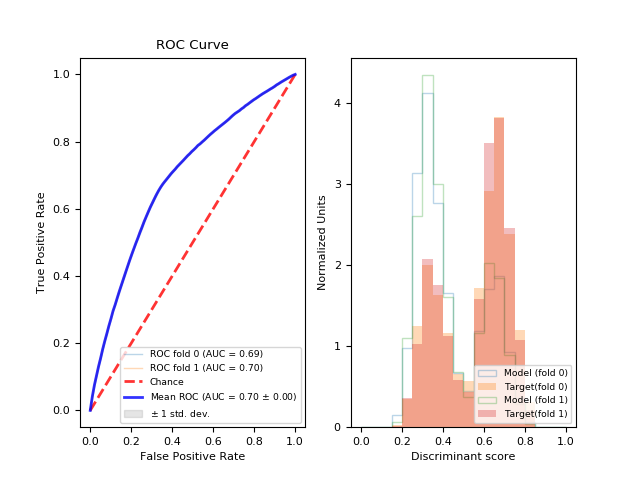
\includegraphics[width=0.50\linewidth]{Figures/Modeling/background/bkgtraining/roc_curve_20172018NonResonantAnalysis_Weight_AnaGGF2_original.png}}
\subfloat[]{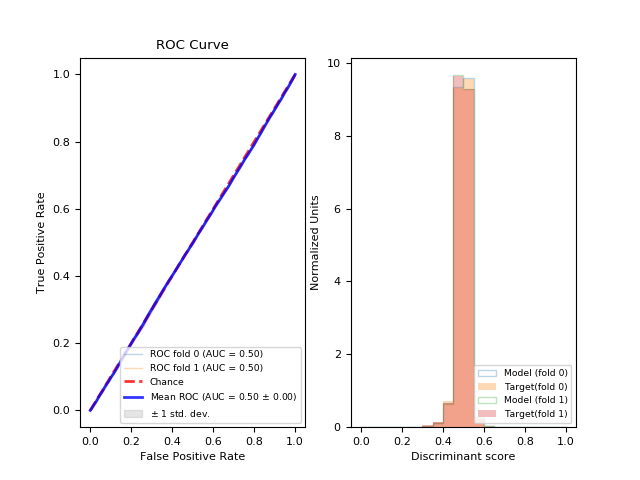
\includegraphics[width=0.50\linewidth]{Figures/Modeling/background/bkgtraining/roc_curve_20172018NonResonantAnalysis_Weight_AnaGGF2_model.png}}
\end{center}
\caption[Example of the discriminant check step in the model for analysis control region data]{Example of the discriminant check step before A) and after B) BDT reweighter weights are applied in the model in control region data. The model corresponds to the one used for the 2017-2018 ggF category 2.}
\label{fig:bkgclassfiercheck}
\end{figure}

Once the BDT-reweighters are trained, their associated weights are applied to re-shape the $\mathrm{A_{CR}}$(3b) distributions and compared to the data $\mathrm{A_{CR}}$(4b) as a closure test. An example of the closure achieved by the BDT reweighting in the control regions can be seen in Figure~\ref{fig:bdtreweightingexampleanalysiscr}. A good closure is observed between data and the background model is observed in all input variables. The distributions are presented in the following figures in Appendix~\ref{appendix:bkgmodel}: Figures~\ref{bkg:fig:bdtregvarggf1_2016} to \ref{bkg:fig:bdtregvarggf2_20172018} for the ggF categories 1 and 2, and the Figures~\ref{bkg:fig:bdtregvarvbf1_2016} to \ref{bkg:fig:bdtregvarvbf1_20172018} for the VBF category 1. 
\clearpage
The derived transfer factors and reweighting rules are applied in the $\mathrm{A_{SR}}$(3b) data to estimate the $\mathrm{A_{SR}}$(4b) background in the observables used for the signal extraction. It is important to emphasize that the methods presented here are optimized and settled without looking at the $\mathrm{A_{SR}}$(4b) data, i.e. a so-called blind analysis is performed. The methods followed a procedure of review within the CMS Collaboration before using the $\mathrm{A_{SR}}$(4b) data to derive the results. Before that, the method is validated in the validation region studies (see Subsection~\ref{sec:bkgvalidation}).

\begin{figure}[htbp!]
\begin{center}
\captionsetup[subfigure]{justification=centering}
\subfloat[]{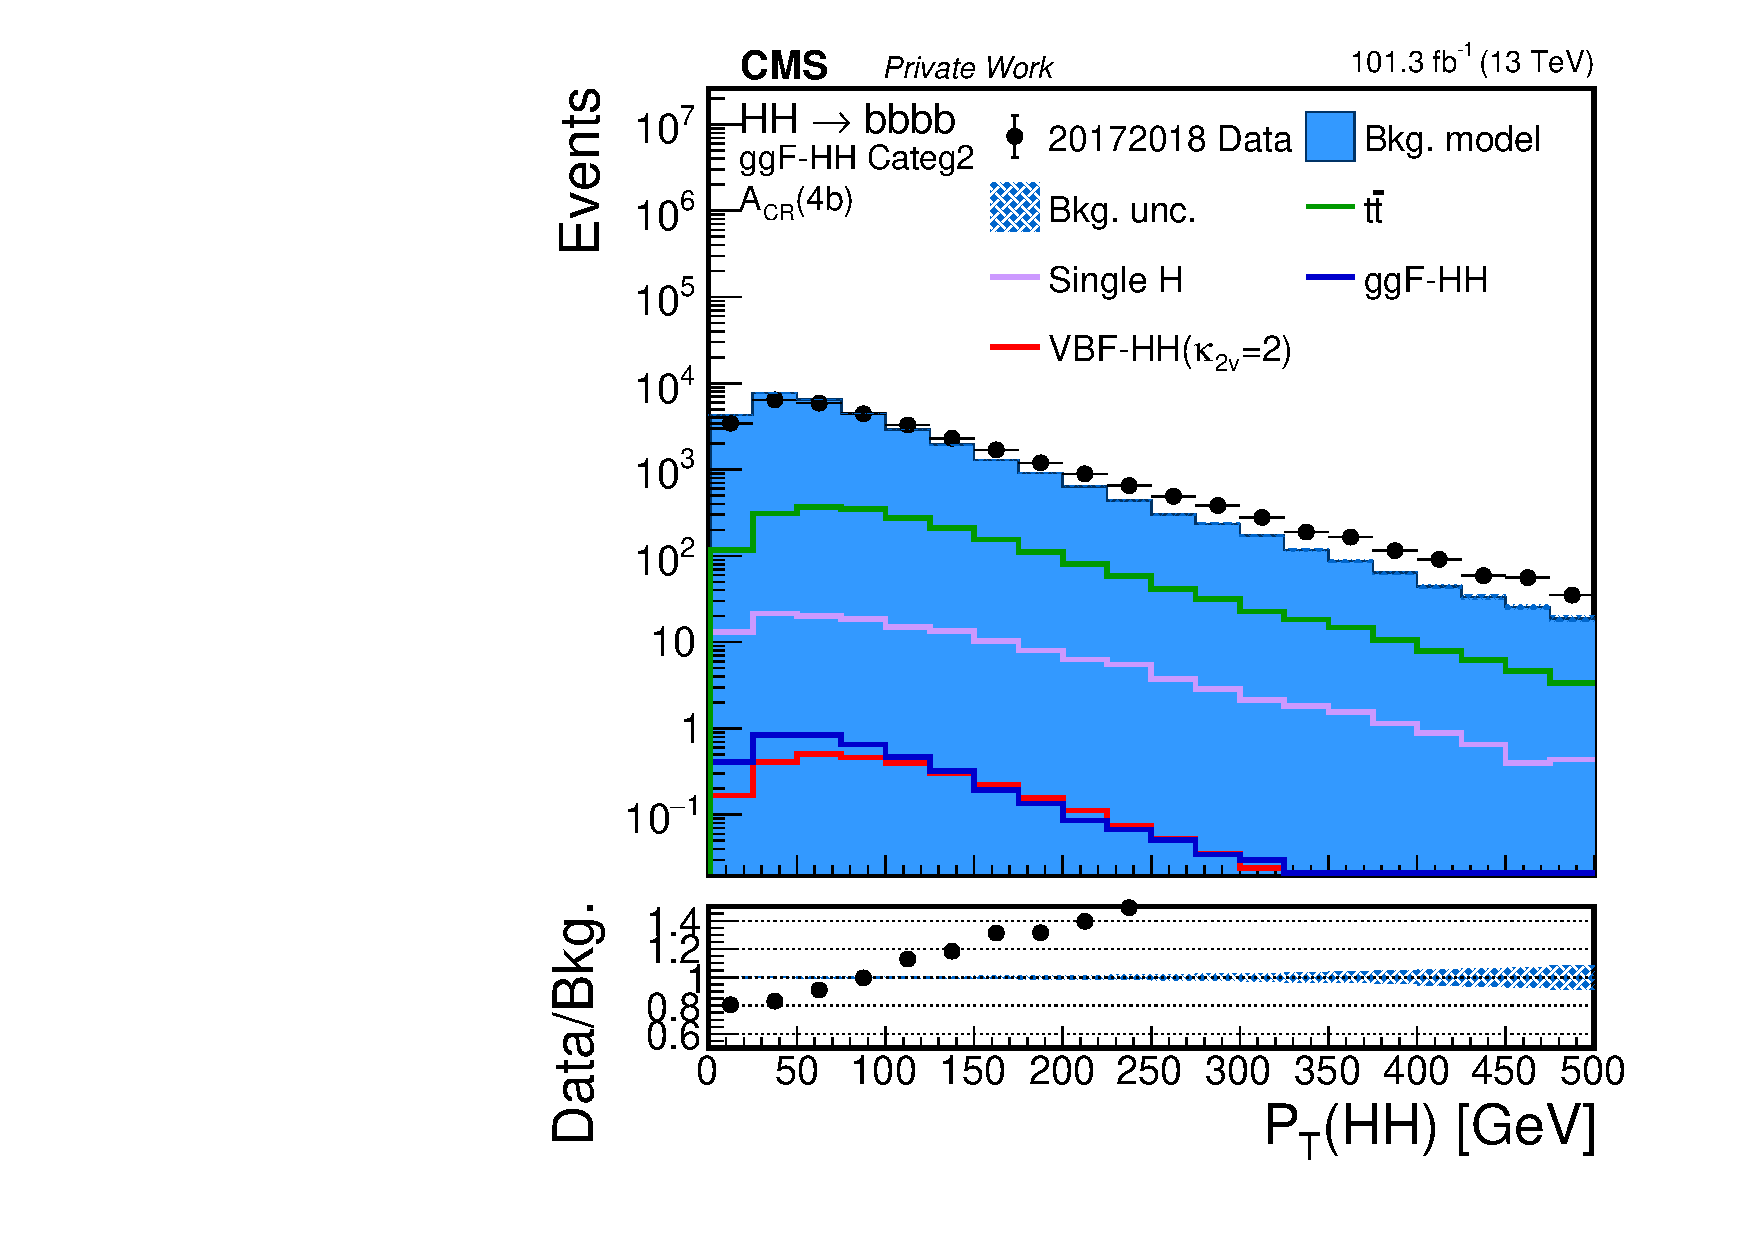
\includegraphics[width=0.45\linewidth]{Figures/Modeling/background/plotsDatadrivenNoBDT/20172018/GGFcateg2_CR_110/Histogram/plot20172018_HH_pt_Btag4_GGFcateg2_CR_110_Histogram_log.pdf}}
\subfloat[]{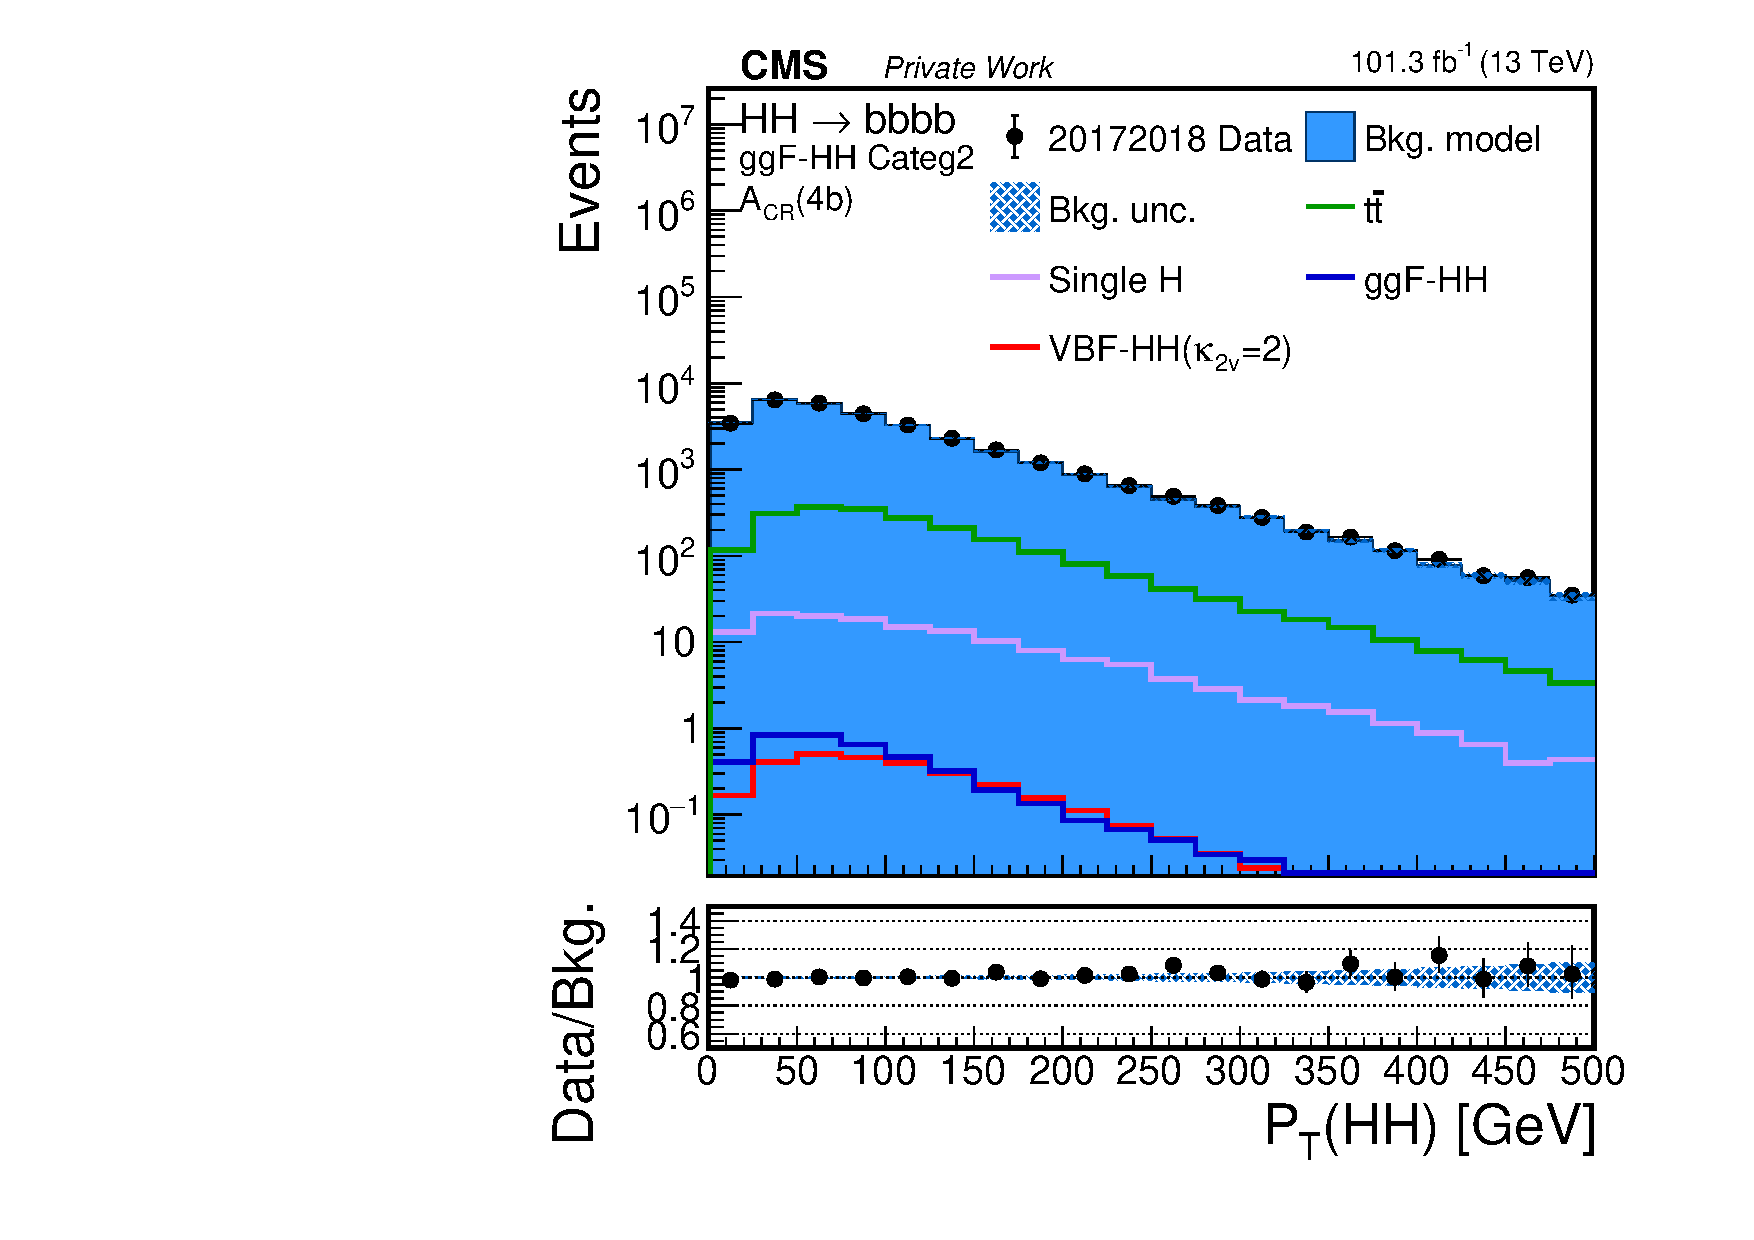
\includegraphics[width=0.45\linewidth]{Figures/Modeling/background/plotsDatadrivenWithBDT/20172018/GGFcateg2_CR_110/Histogram/plot20172018_HH_pt_Btag4_GGFcateg2_CR_110_Histogram_log.pdf}}
\end{center}
\caption[Example of the data versus background modeling agreement in 20172018 ggF category 2]{Example of data versus background modeling agreement without A) and with B) BDT reweighting in the analysis control regions data of the 20172018 ggF category 2.}
\label{fig:bdtreweightingexampleanalysiscr}
\end{figure}

\subsection{Validation Studies} \label{sec:bkgvalidation}
The background model technique is fully validated by studying it in a region orthogonal to the $\mathrm{A_{SR}}$ region and with a comparable statistical power. In essence, a transfer model is derived using the validation control regions defined in Subsection~\ref{sec:analysisregions}: $\mathrm{V_{CR}}$(3b) and $\mathrm{V_{CR}}$(4b). Then, the transfer model is applied to the $\mathrm{V_{SR}}$(3b) data to model the background in the $\mathrm{V_{SR}}$(4b) data. First, the validation produce consists in checking the closure of the background normalization and reweighting with the observed data in the $\mathrm{V_{SR}}$(4b) region. Moreover, the closure of all observables used for the signal extraction is tested.

\subsubsection{Normalization validation test}

Tables~\ref{bkg:tab:valfactor1} and \ref{bkg:tab:valfactor2} present the observed data and expected background normalization values for all categories in the 2016 and 2017-2018 data. The sources of the $\mathrm{N(V_{SR}^{4b})_{pred}}$ uncertainty are: the statistical uncertainty from the SR(3b) data and the normalization transfer factor $\alpha$ from the control regions, respectively. One can see that the transfer factor model is able to predict correctly the normalization within the uncertainties. There are some categories with a residual difference at the order of up to two standard deviations, which are considered as a systematic uncertainty during the statistical analysis in the $\mathrm{A_{SR}}$(4b) region. 

\begin{table}[htb]
\caption[Summary of the transfer factor and normalization estimation in the 2016 validation test]{\label{bkg:tab:valfactor1}Summary of the transfer factor and normalization estimation in the 2016 validation study. The normalization used in the background model is denoted as $\mathrm{N(V_{SR}^{4b})_{pred}}$.}
\small
\centering
\begin{tabularx}{\textwidth}{l r r r r}
    \hline
    Subcategory                                 &   ggF Cat1               & ggF Cat2                & VBF Cat1                 & VBF Cat2              \\
    \hline
    $\mathrm{N(V_{CR}^{3b})}$                   &  58203$\pm$241.3         & 190979$\pm$437.0        &  6146$\pm$78.4           &     90$\pm$9.5        \\
    $\mathrm{N(V_{SR}^{3b})}$                   &  30703$\pm$175.2         &  70566$\pm$265.6        &  2257$\pm$47.5           &     30$\pm$5.5        \\
    $\mathrm{N(V_{CR}^{4b})}$                   &   6108$\pm$ 78.2         &  16775$\pm$129.5        &   857$\pm$29.3           &      9$\pm$3.0        \\
    $\mathrm{N(V_{SR}^{4b})}$                   &   3349$\pm$ 57.9         &   6062$\pm$77.8         &   317$\pm$17.8           &      1$\pm$1.0  \\
    $\alpha$                                    & 0.10494$\pm$0.00141      &0.08784$\pm$0.0007       &0.13944$\pm$0.00508       &    0.1$\pm$0.03496    \\
    $\mathrm{N(V_{SR}^{4b})_{\alpha}}$          &  3222.1$\pm$23.6$\pm$43.3& 6198.3$\pm$29.7$\pm$49.4&  314.7$\pm$6.8$\pm$11.5  &    3.0$\pm$0.5$\pm$1.0\\
    $\mathrm{N(V_{SR}^{4b})_{\alpha,\parallel}}$&  3207.6$\pm$23.5$\pm$73.1& 6088.8$\pm$29.2$\pm$77.4&         -                &  -                    \\
    $\mathrm{N(V_{SR}^{4b})_{pred}}$            &  3207.6$\pm$23.5$\pm$73.1& 6088.8$\pm$29.2$\pm$77.4&  314.7$\pm$6.8$\pm$11.5  &    3.0$\pm$0.5$\pm$1.0\\
    \hline
\end{tabularx}
\end{table}

\begin{table}[htb]
\caption[Summary of the transfer factor and normalization estimation in the 2017-2018 validation test]{\label{bkg:tab:valfactor2}Summary of the transfer factor and normalization estimation in the 2017-2018 validation study. The normalization used in the background model is denoted as $\mathrm{N(A_{SR}^{4b})_{pred}}$.}
\small
\centering
\begin{tabularx}{\textwidth}{l r r r r}
    \hline
    Subcategory                                  &   ggF Cat1               & ggF Cat2                & VBF Cat1                  & VBF Cat2              \\
    \hline
    $\mathrm{N(V_{CR}^{3b})}$                    &  72379$\pm$269.0         & 260855$\pm$510.7        & 11194$\pm$105.8           &    192$\pm$13.9       \\
    $\mathrm{N(V_{SR}^{3b})}$                    &  38387$\pm$195.9         &  88771$\pm$297.9        &  3980$\pm$ 63.1           &     51$\pm$7.1        \\
    $\mathrm{N(V_{CR}^{4b})}$                    &  10967$\pm$104.7         &  29842$\pm$172.7        &  1864$\pm$ 43.2           &     23$\pm$4.8        \\
    $\mathrm{N(V_{SR}^{4b})}$                    &   5981$\pm$77.3          &  10254$\pm$101.3        &   670$\pm$ 25.9           &      4$\pm$2.0        \\    
    $\alpha$                                     & 0.15152$\pm$0.00155      &0.11440$\pm$0.00070      &0.16652$\pm$0.00417        &0.11979$\pm$0.02643    \\
    $\mathrm{N(V_{SR}^{4b})_{\alpha}}$           &  5816.4$\pm$36.4$\pm$59.5&10155.5$\pm$41.4$\pm$62.1&  662.7$\pm$11.1$\pm$16.6  &    6.1$\pm$0.9$\pm$1.3\\
    $\mathrm{N(V_{SR}^{4b})_{\alpha,\parallel}}$ &  5683.3$\pm$35.6$\pm$95.5&10042.3$\pm$40.9$\pm$98.7&         -                 &         -             \\
    $\mathrm{N(V_{SR}^{4b})_{pred}}$             &  5683.3$\pm$35.6$\pm$95.5&10042.3$\pm$40.9$\pm$98.7&  662.7$\pm$11.1$\pm$16.6  &    6.1$\pm$0.9$\pm$1.3\\
    \hline
\end{tabularx}
\end{table}

\subsubsection{BDT reweighting validation test}
This test aims at checking that the BDT reweighting method derived in control regions performs well when is applied to the signal region. To this end, BDT-reweighters are trained using the same procedure as in the analysis region, but instead using the $\mathrm{V_{CR}}$ information. An example of the discriminant check of the validation training is shown in Figure~\ref{fig:bkgclassfiercheckval} for the 2017-2018 ggF category 2. The optimized hyperparameters are presented in Tables~\ref{bkg:tab:bdtregparametersval2016} and \ref{bkg:tab:bdtregparametersval20172018}  in Appendix~\ref{appendix:bkgmodel}.
\begin{figure}[htbp!]
\begin{center}
\captionsetup[subfigure]{justification=centering}
\subfloat[]{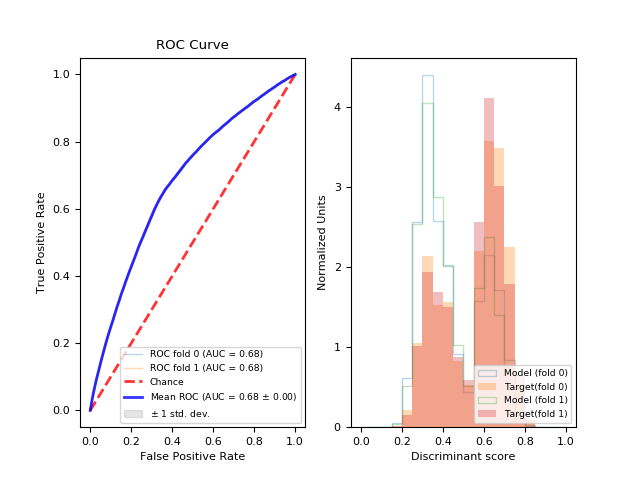
\includegraphics[width=0.47\linewidth]{Figures/Modeling/background/bkgtraining/roc_curve_20172018NonResonantAnalysis_Weight_ValGGF2_original.png}}
\subfloat[]{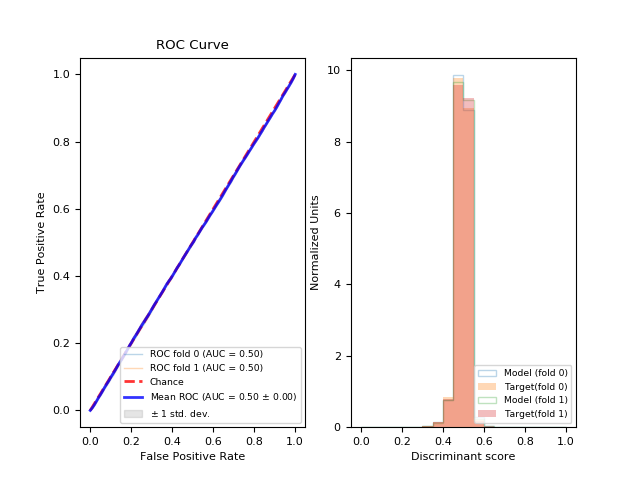
\includegraphics[width=0.47\linewidth]{Figures/Modeling/background/bkgtraining/roc_curve_20172018NonResonantAnalysis_Weight_ValGGF2_model.png}}
\end{center}
\caption[Example of the discriminant check step in the model for validation control region data]{Example of the discriminant check step before A) and after B) BDT reweighter weights are applied in the model in validation control region data. The model corresponds to the one used for the 2017-2018 ggF category 2.}
\label{fig:bkgclassfiercheckval}
\end{figure}

After the BDT-reweighters are trained, the weights are applied to the $\mathrm{V_{CR}}$(3b) events to model $\mathrm{V_{CR}}$(4b) ones. A very good agreement is observed between the data and the model in all variables involved in the $\mathrm{V_{CR}}$ reweighting. The reweighting variables distributions of data and the background model are illustrated for ggF categories in Figures~\ref{bkg:fig:valbdtregvarggf1_2016}-\ref{bkg:fig:valbdtregvarggf2_20172018} and for VBF category in Figures~\ref{bkg:fig:valbdtregvarvbf1_2016}-\ref{bkg:fig:valbdtregvarvbf1_20172018}. The improvement achieved from the BDT-reweighting in the $\mathrm{V_{CR}}$(4b) region is illustrated for one of the reweighting variables in Figure~\ref{fig:bdtreweightingexamplevalidationcr}.

The BDT reweighting method is then checked by studying the application of the method in the $\mathrm{V_{SR}}$ region. A good agreement between the observed data and  background model in all variables involved in the re-weighting is observed in the $\mathrm{V_{SR}}$(4b) region. Figures~\ref{bkg:fig:valsrbdtregvarggf1_2016} to \ref{bkg:fig:valsrbdtregvarggf2_20172018} present the performance of our background estimate in the ggF $\mathrm{V_{SR}}$ regions, whereas Figures~\ref{bkg:fig:valsrbdtregvarvbf1_2016} to \ref{bkg:fig:valsrbdtregvarvbf1_20172018} present the performance of our background estimate in the VBF $\mathrm{V_{SR}}$ regions. The improvement with respect to the case without reweighting is illustrated in Figure~\ref{fig:bdtreweightingexamplevalidationsr}. These results show that the data-driven technique is capable of accurately modeling the background in the signal regions of the analysis.

\begin{figure}[ht!]
\begin{center}
\captionsetup[subfigure]{justification=centering}
\subfloat[]{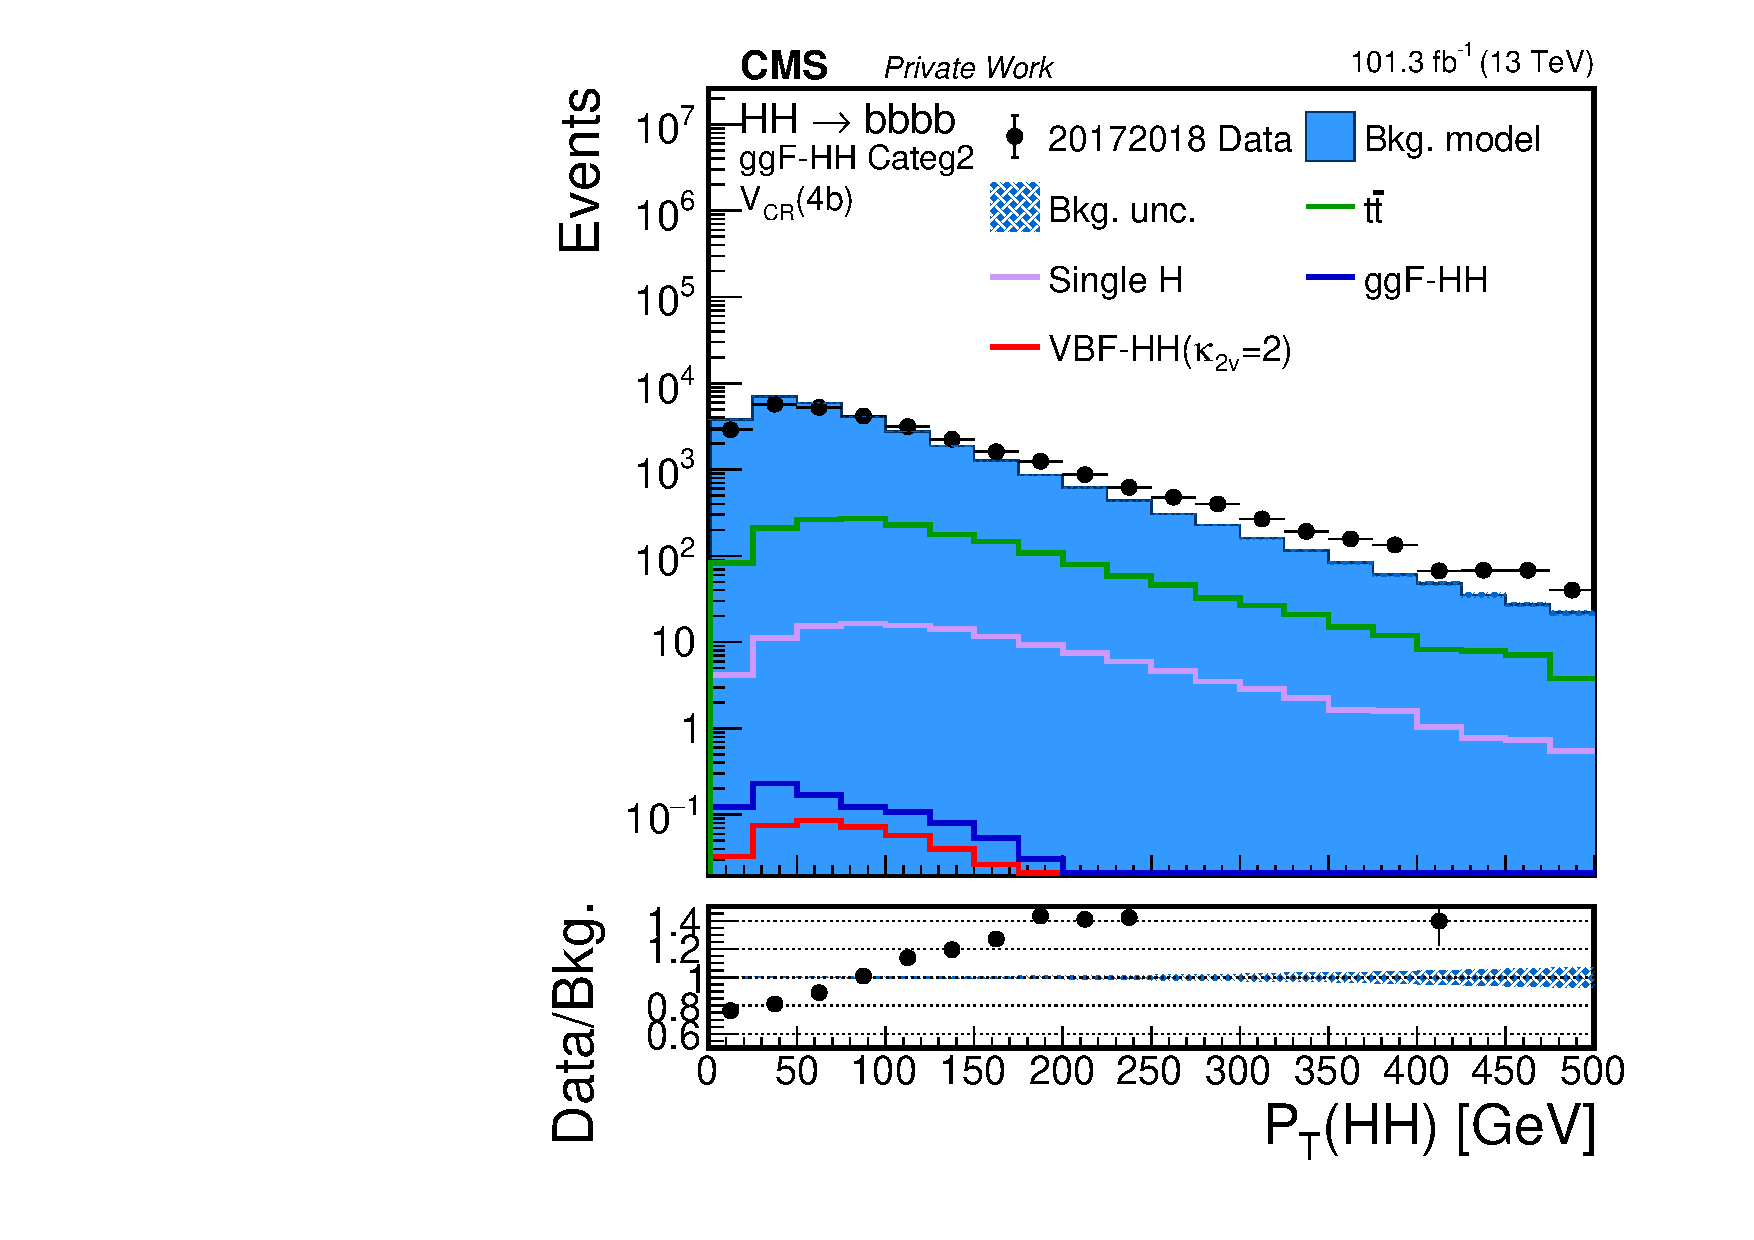
\includegraphics[width=0.48\linewidth]{Figures/Modeling/background/plotsDatadrivenNoBDT/20172018/GGFcateg2_CR_210/Histogram/plot20172018_HH_pt_Btag4_GGFcateg2_CR_210_Histogram_log.pdf}}
\subfloat[]{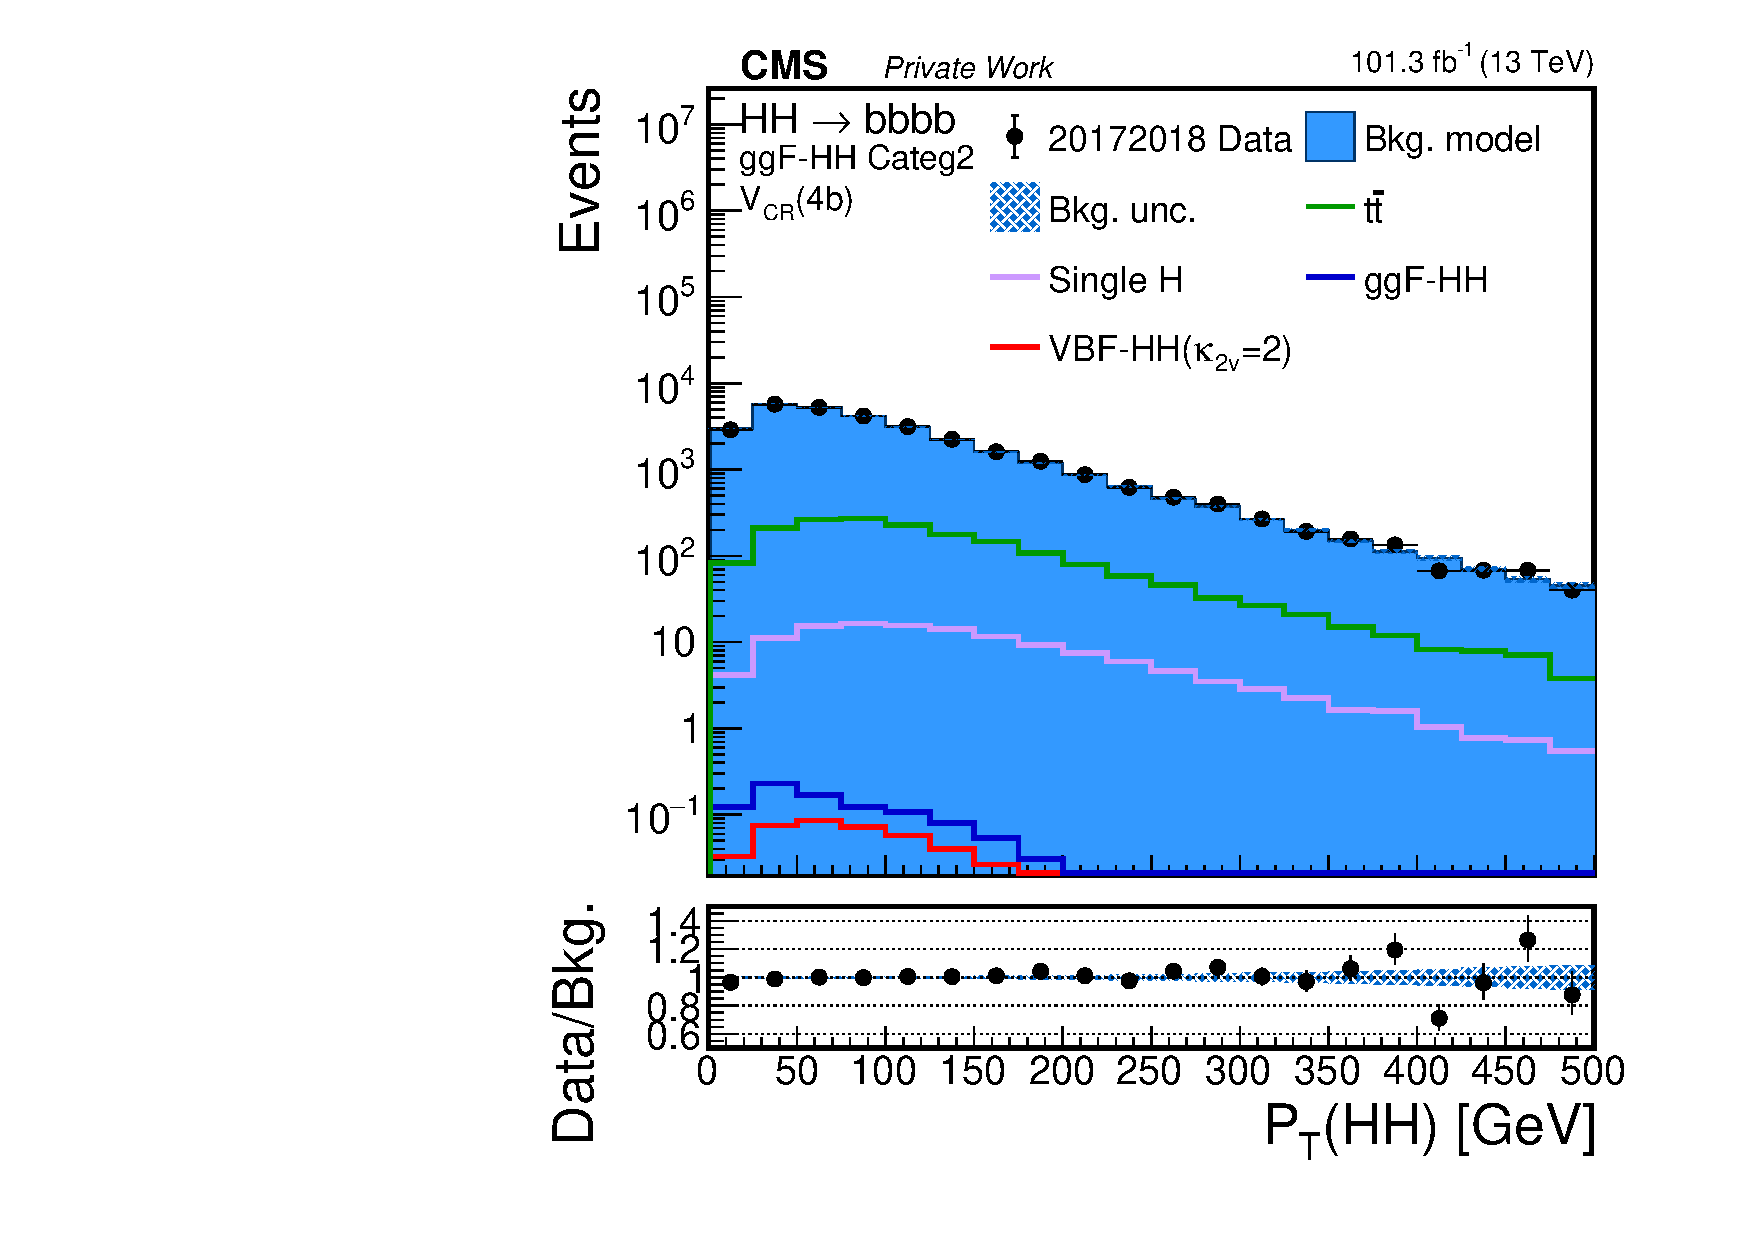
\includegraphics[width=0.48\linewidth]{Figures/Modeling/background/plotsDatadrivenWithBDT/20172018/GGFcateg2_CR_210/Histogram/plot20172018_HH_pt_Btag4_GGFcateg2_CR_210_Histogram_log.pdf}}
\end{center}
\caption[Example of the data versus background modeling agreement in 20172018 ggF category 2 validation control region]{Example of data versus background modeling agreement A) without and B) with BDT reweighting in the validation control region of the 20172018 ggF category 2.}
\label{fig:bdtreweightingexamplevalidationcr}
\end{figure}

\begin{figure}[ht!]
\begin{center}
\captionsetup[subfigure]{justification=centering}
\subfloat[]{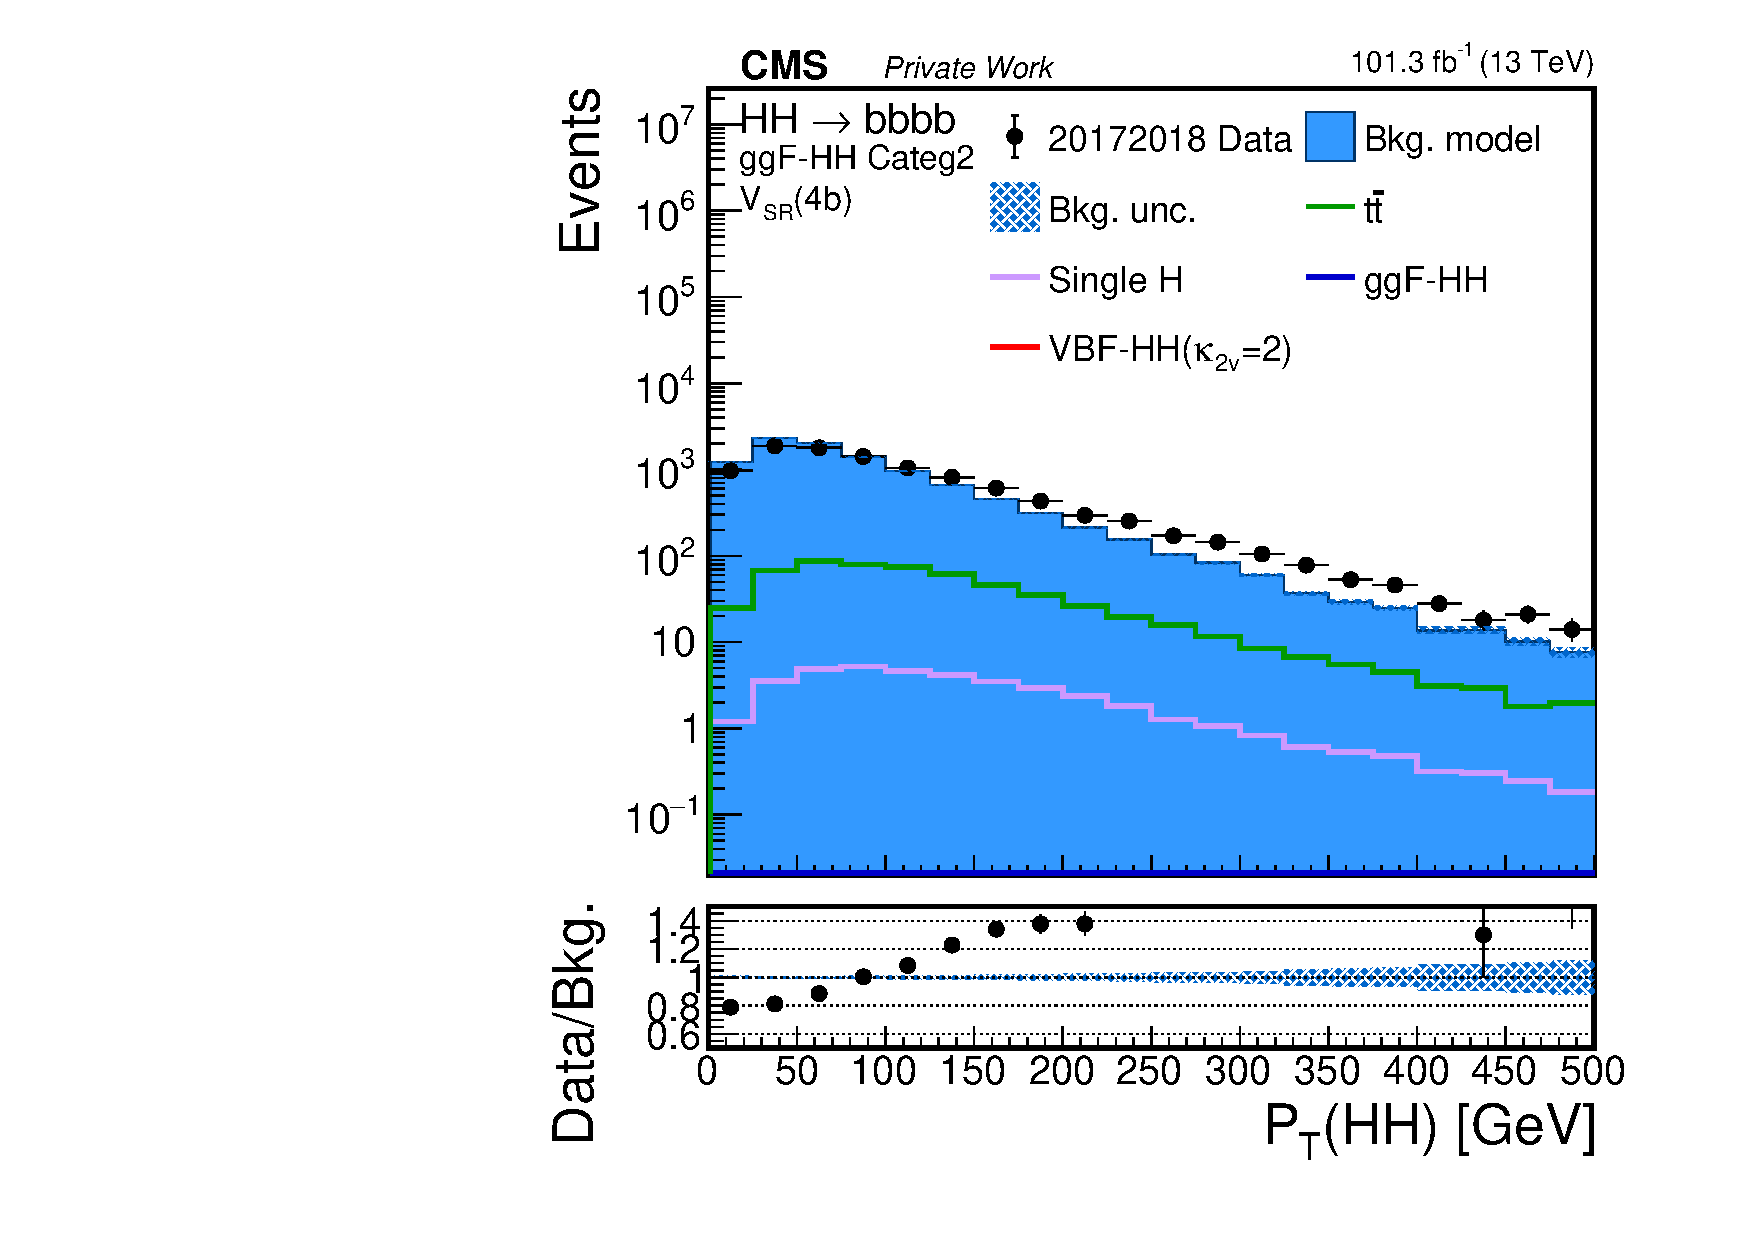
\includegraphics[width=0.48\linewidth]{Figures/Modeling/background/plotsDatadrivenNoBDT/20172018/GGFcateg2_SR_210/Histogram/plot20172018_HH_pt_Btag4_GGFcateg2_SR_210_Histogram_log.pdf}}
\subfloat[]{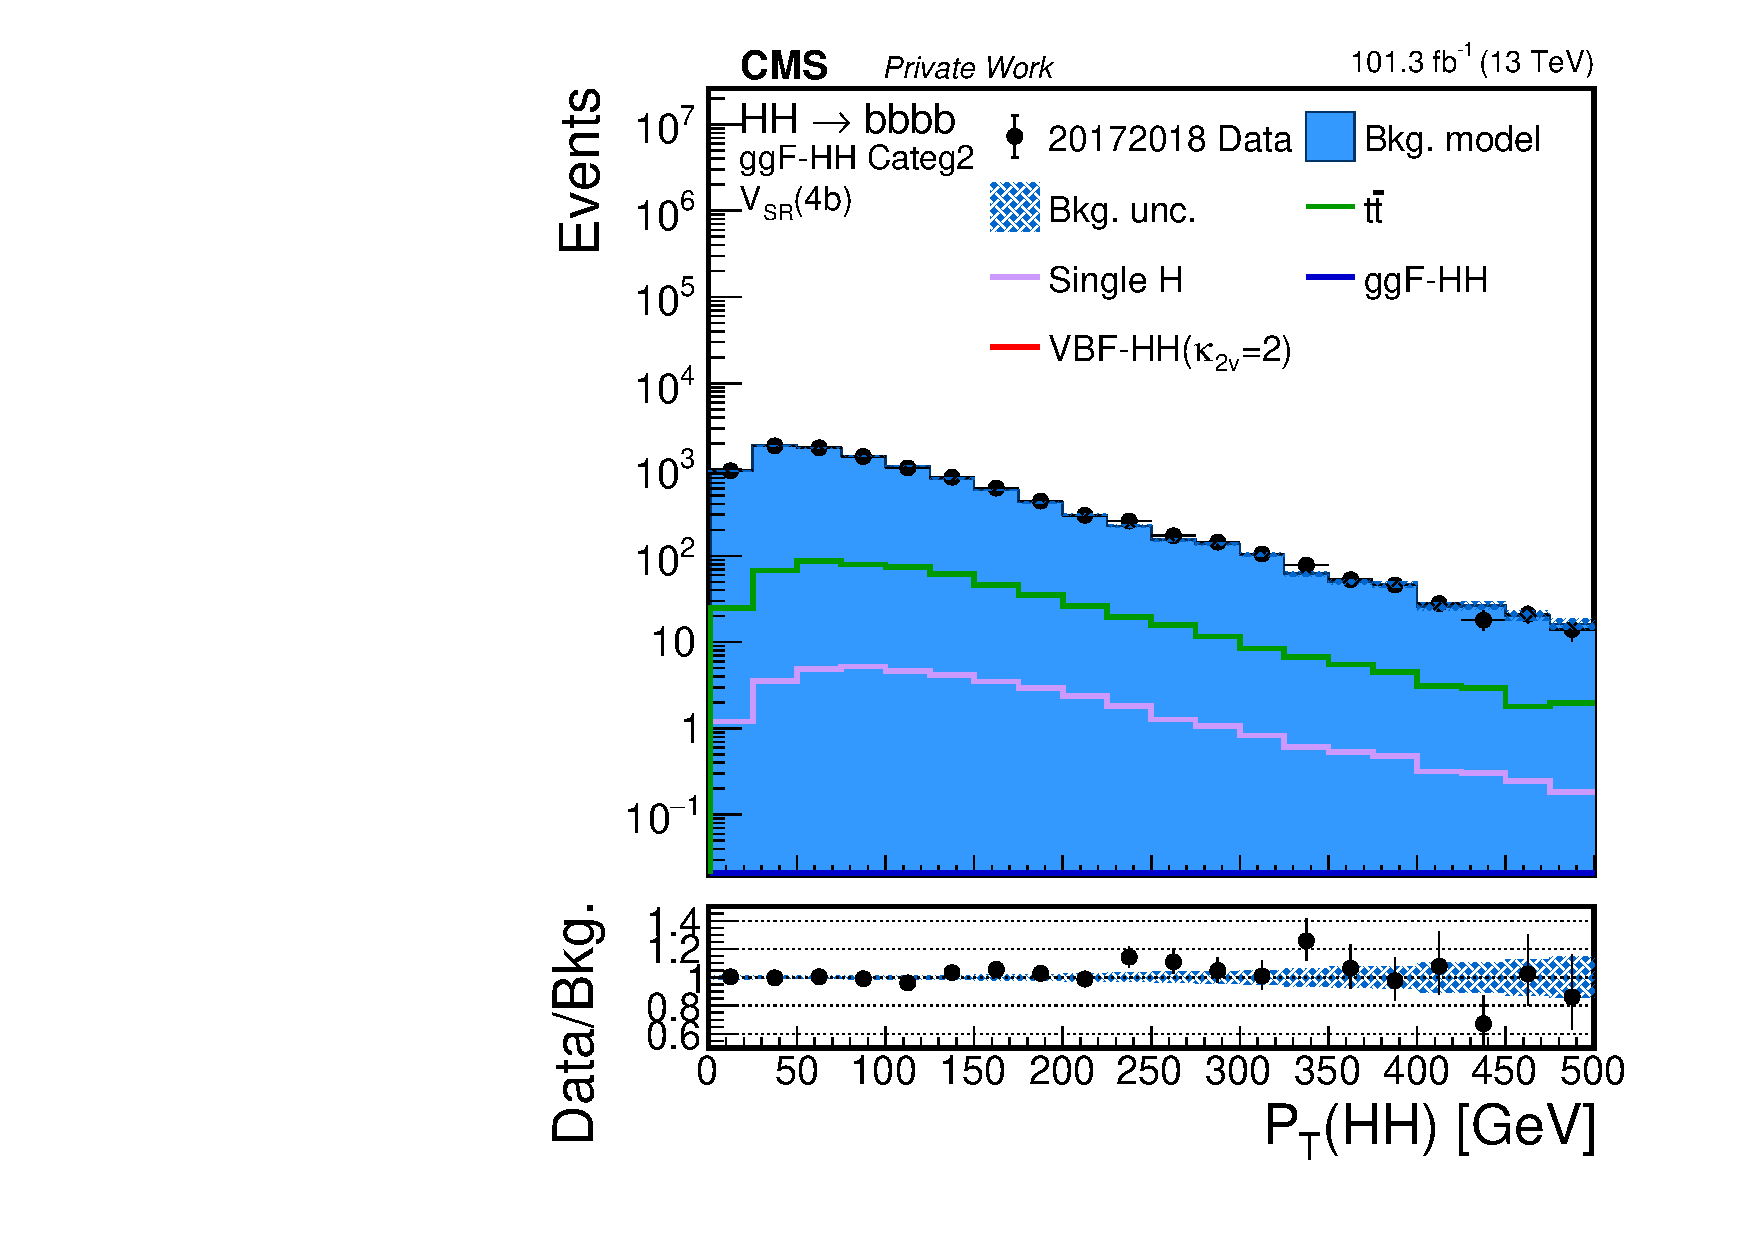
\includegraphics[width=0.48\linewidth]{Figures/Modeling/background/plotsDatadrivenWithBDT/20172018/GGFcateg2_SR_210/Histogram/plot20172018_HH_pt_Btag4_GGFcateg2_SR_210_Histogram_log.pdf}}
\end{center}
\caption[Example of the data versus background modeling agreement in 20172018 ggF category 2 validation control region]{Example of data versus background modeling agreement without A) and with B) BDT reweighting in the validation signal region of the 2017-2018 ggF category 2.}
\label{fig:bdtreweightingexamplevalidationsr}
\end{figure}

\clearpage

\subsubsection{Statistical closure test in the validation region}
As presented in Chapter~\ref{chapter:results}, the signal extraction is performed in eight observables associated to four subcategories in two datasets. One crucial test is to confirm that the background estimate models well the data in all the observables. However, this is not possible to do this before $\mathrm{A_{SR}}$(4b)  unblinding approval. Consequently, this test is performed in the $\mathrm{V_{SR}}$(4b) region. 

The closure test consists on studying the observables by performing a background-only fit to the observed data by floating the background nuisance parameters and their uncertainties (more in~\ref{chapter:results}). For each observable, the post-fit background model is compared to the observed data in order to check that there are not any striking trends pointing to a mismodeling. The resulting $\mathrm{V_{SR}}$(4b) distributions are illustrated in Figure~\ref{fig:bkgobservablesvaltest2016} and Figure~\ref{fig:bkgobservablesvaltest2016} for 2016 and 2017-2018 data, respectively. A very good agreement is observed across all observables.

In addition, a goodness of fit test based on the saturated method~\cite{statsaturatedmodel} is performed in each observable to quantify the compatibility between the background model and observed data. A high compatibility (p-value$>5\%$) is observed across all observables of the $\mathrm{V_{SR}}$(4b) region, as presented in Table~\ref{tab:valcompatibilty}. A similar test is carried out during the unblinding of the $\mathrm{A_{SR}}$(4b) region observables, and further described in Section~\ref{results:modelvalidation}.

\begin{table}[htbp!]
\caption[Data-background model compatibility p-value obtained from the goodness of fit test in the validation region]{\label{tab:valcompatibilty} Data-background model compatibility p-value obtained from the goodness of fit test applied to the observables in the $\mathrm{V_{SR}}$(4b) regions.}
\centering

\begin{tabularx}{\textwidth}{l l X X}
    \hline
    Dataset          & Subcategory    & Observable           &  Goodness of fit test p-value \\    
    \hline
    2016      & ggF category 1 & BDT output (GGFMVA1) & 42\% \\
    2016      & ggF category 2 & BDT output (GGFMVA2) & 57\% \\
    2016      & VBF category 1 & $\hhm$               & 55\% \\
    2016      & VBF category 2 & Counting experiment  & 22\% \\
    2017-2018 & ggF category 1 & BDT output (GGFMVA1) & 45\% \\
    2017-2018 & ggF category 2 & BDT output (GGFMVA2) & 12\% \\
    2017-2018 & VBF category 1 & $\hhm$               & 83\% \\
    2017-2018 & VBF category 2 & Counting experiment  & 42\% \\
    Run-2     & All            & All                  & 53\% \\ 
    \hline
\end{tabularx}
\end{table}

\begin{figure}[htbp!]
\begin{center}
\captionsetup[subfigure]{justification=centering}
\subfloat[]{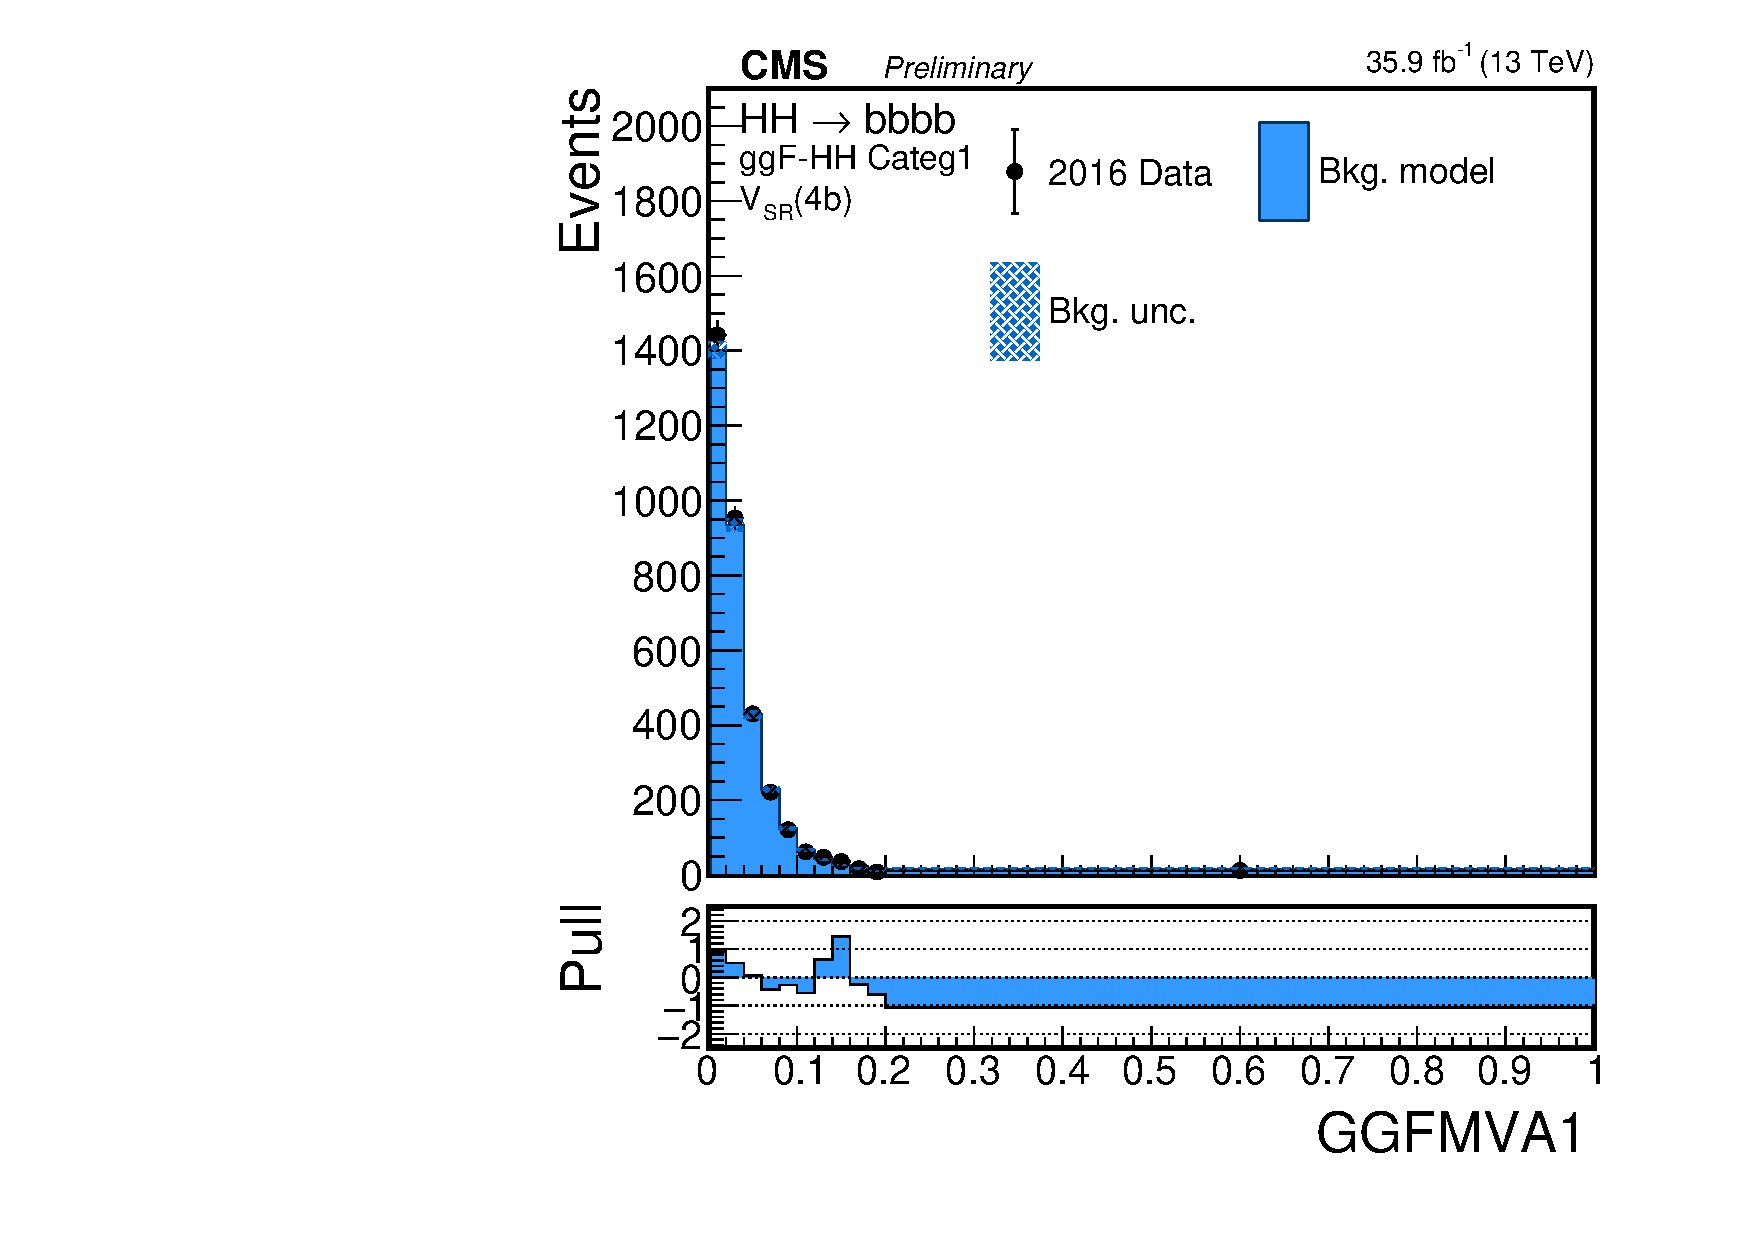
\includegraphics[width=0.48\linewidth]{Figures/Modeling/background/validationobservables/2016/plot2016_GGFMVA1_Btag4_GGFcateg1_SR_210_Histogram_postfit.pdf}}
\subfloat[]{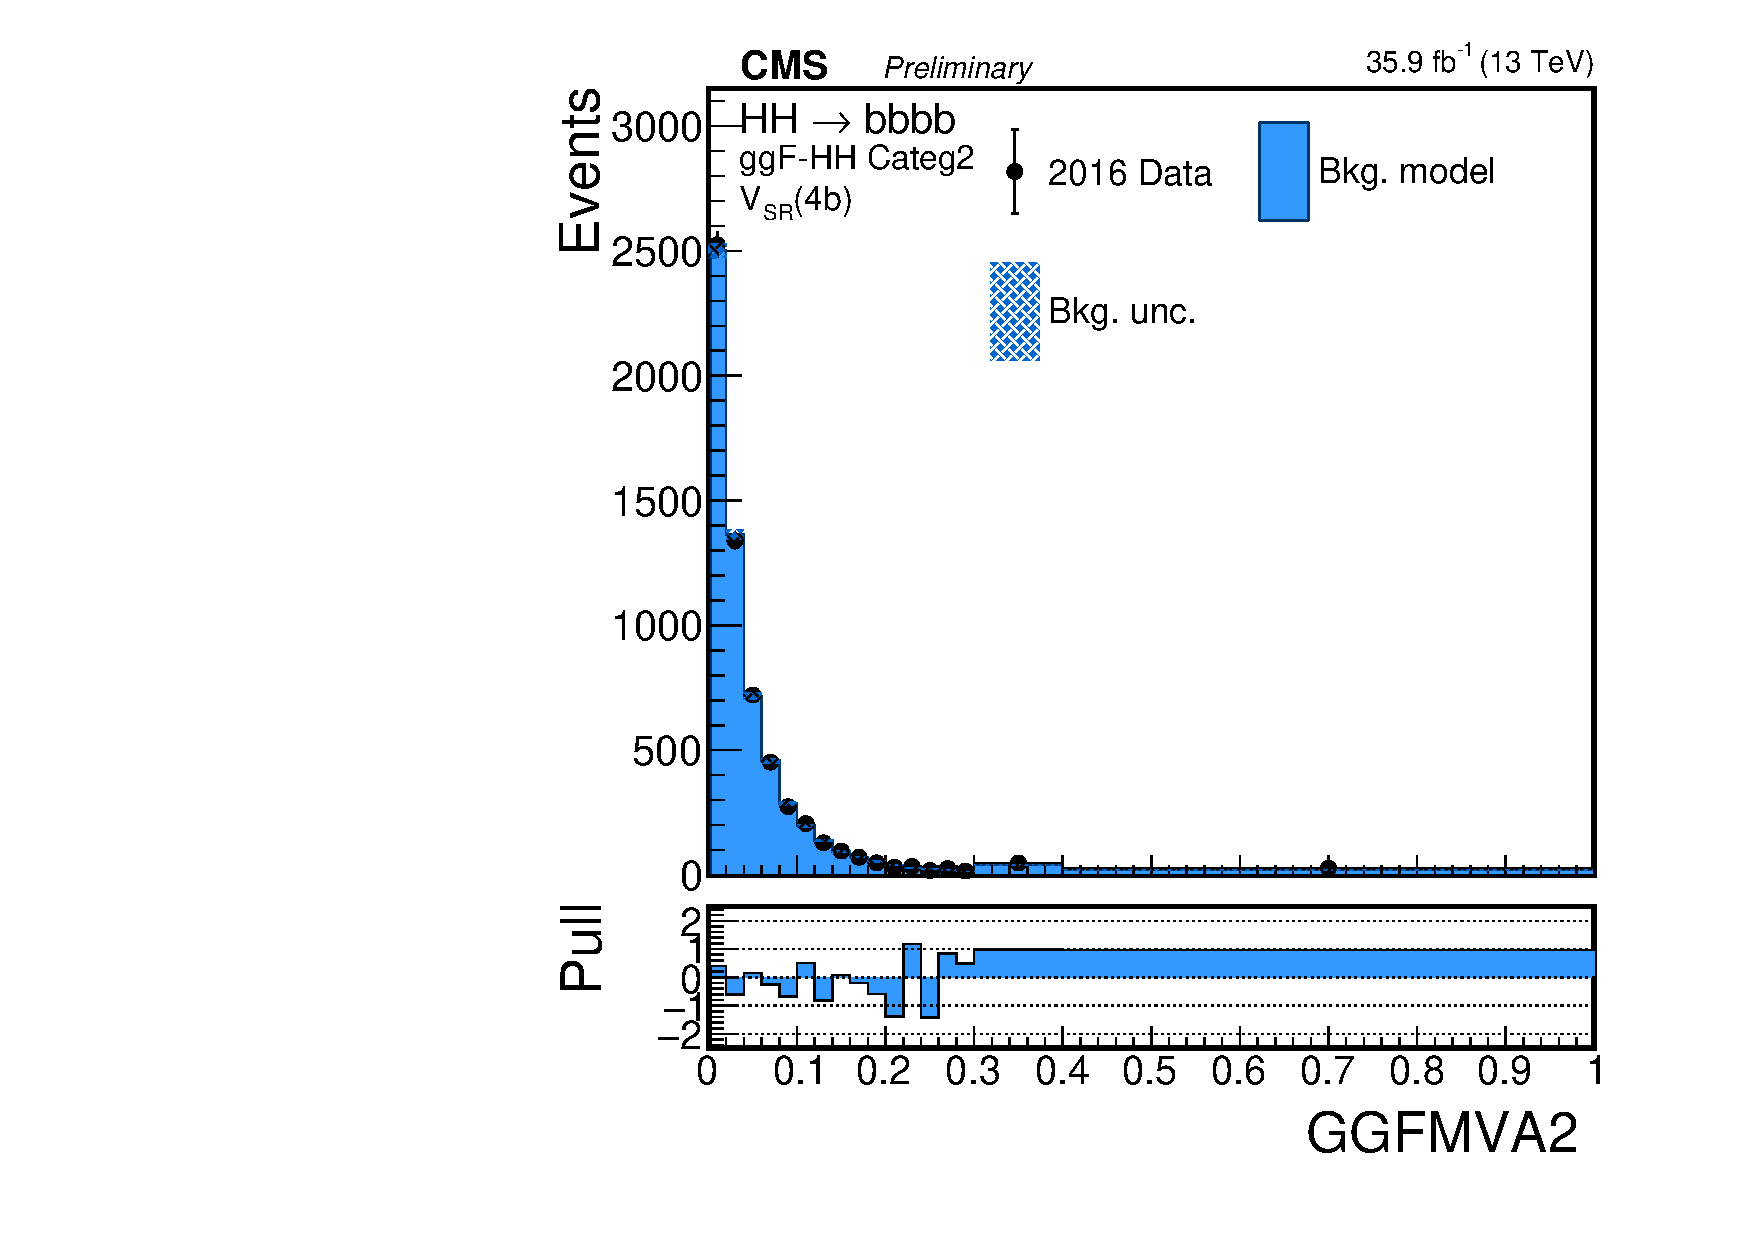
\includegraphics[width=0.48\linewidth]{Figures/Modeling/background/validationobservables/2016/plot2016_GGFMVA2_Btag4_GGFcateg2_SR_210_Histogram_postfit.pdf}}\\
\subfloat[]{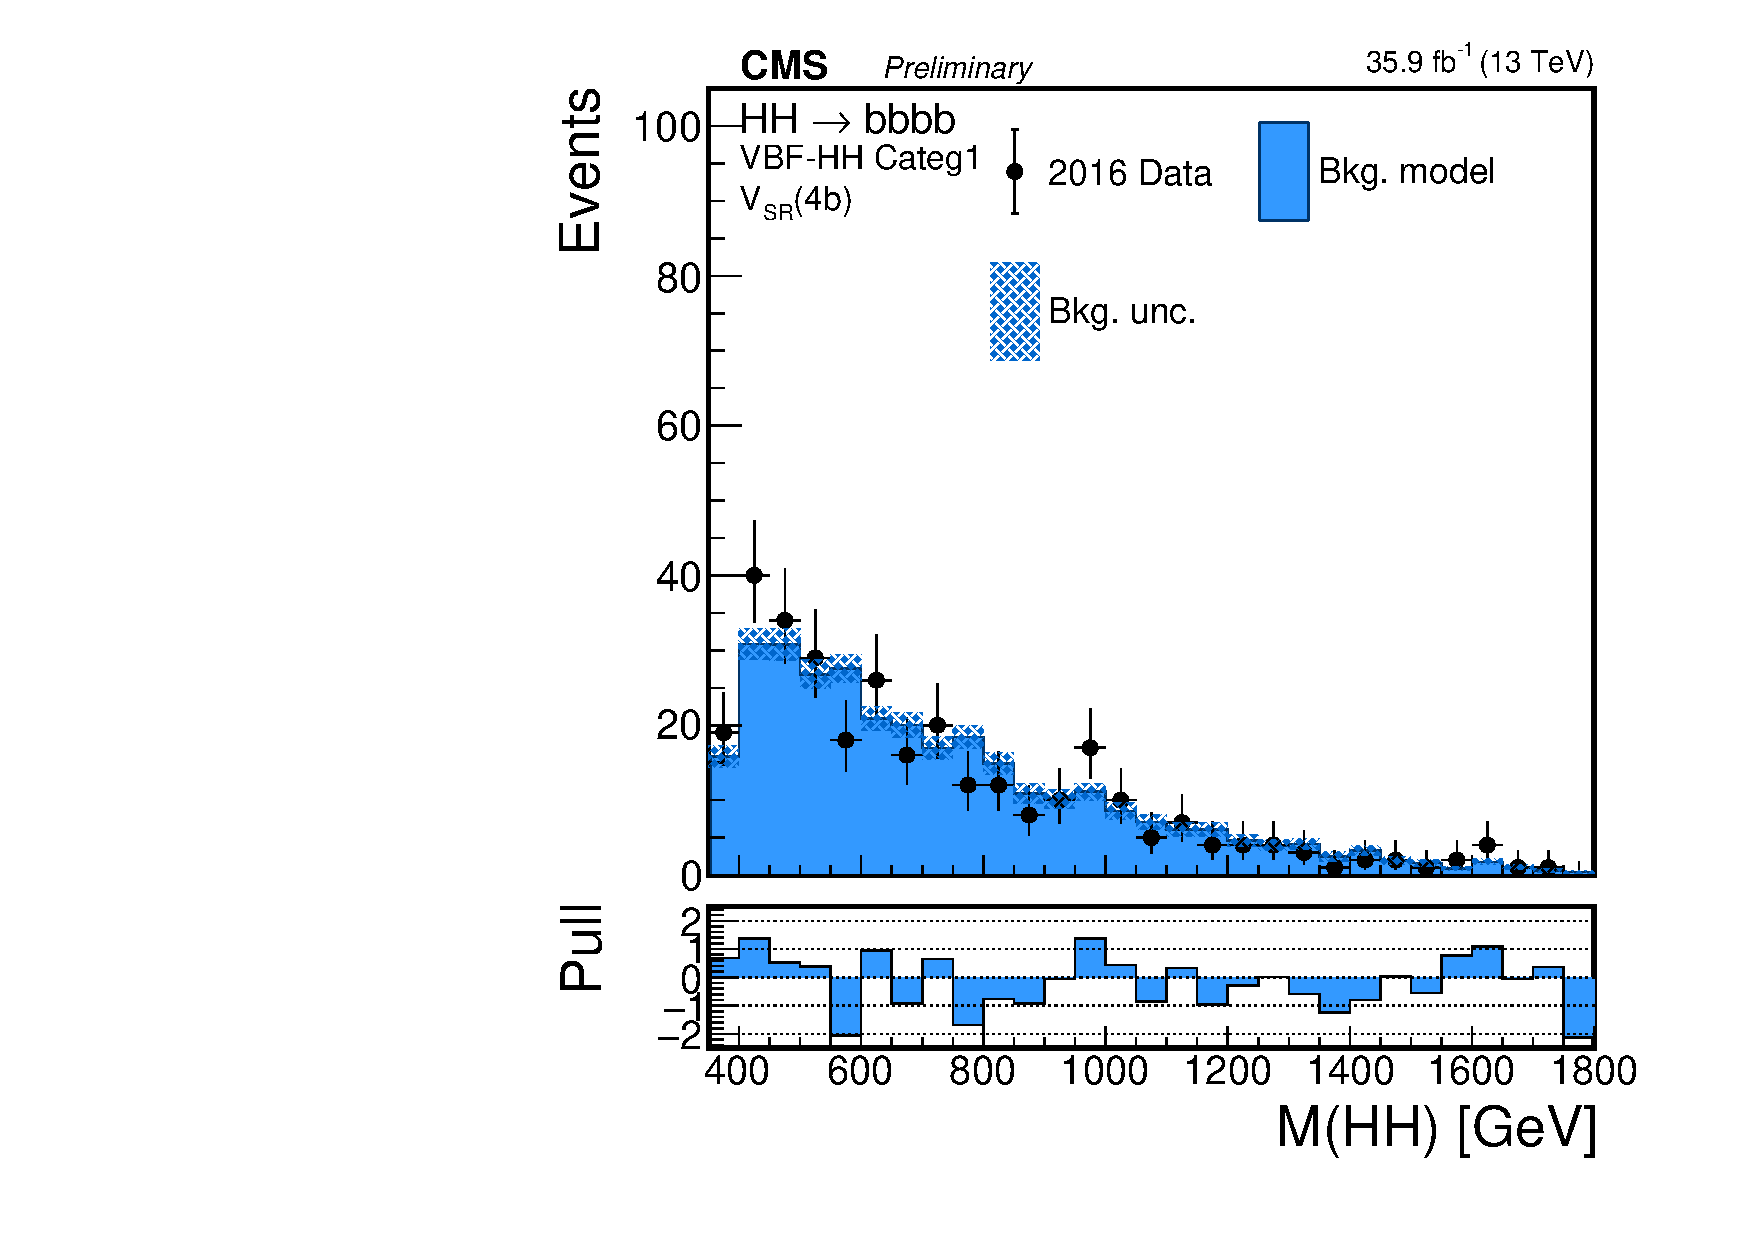
\includegraphics[width=0.48\linewidth]{Figures/Modeling/background/validationobservables/2016/plot2016_HH_m_1_Btag4_VBFcateg1_SR_210_Histogram_postfit.pdf}}
\subfloat[]{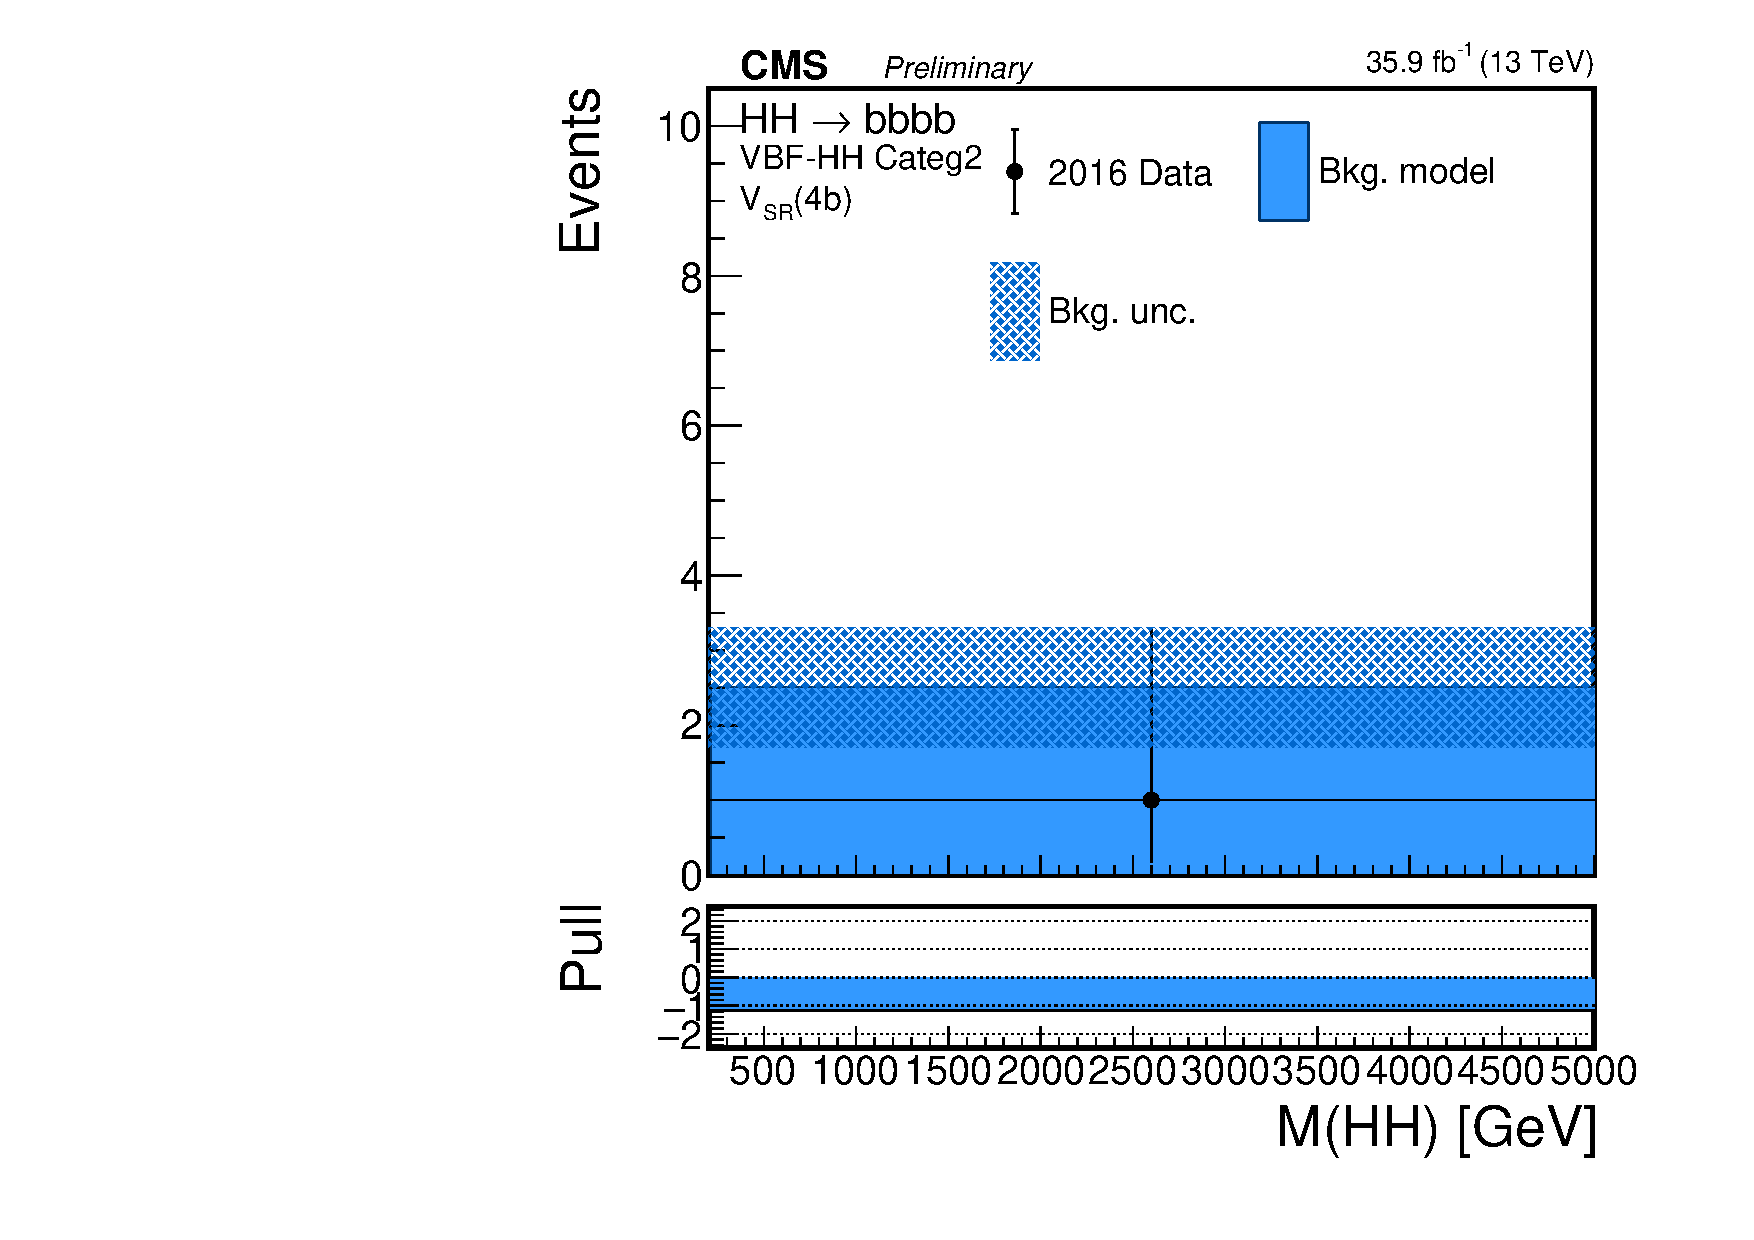
\includegraphics[width=0.48\linewidth]{Figures/Modeling/background/validationobservables/2016/plot2016_HH_m_2_Btag4_VBFcateg2_SR_210_Histogram_postfit.pdf}}
\end{center}
\caption[Distributions of the observables in all validation signal regions for 2016 data]{Distributions of the observables in all validation signal regions for 2016 data. A) ggF category 1, B) ggF category 2, C) VBF category 1, D) VBF Category 2. The presented background distributions are the one obtained after fitting the background prediction to the data floating the background uncertainties.}
\label{fig:bkgobservablesvaltest2016}
\end{figure}

\begin{figure}[htbp!]
\begin{center}
\captionsetup[subfigure]{justification=centering}
\subfloat[]{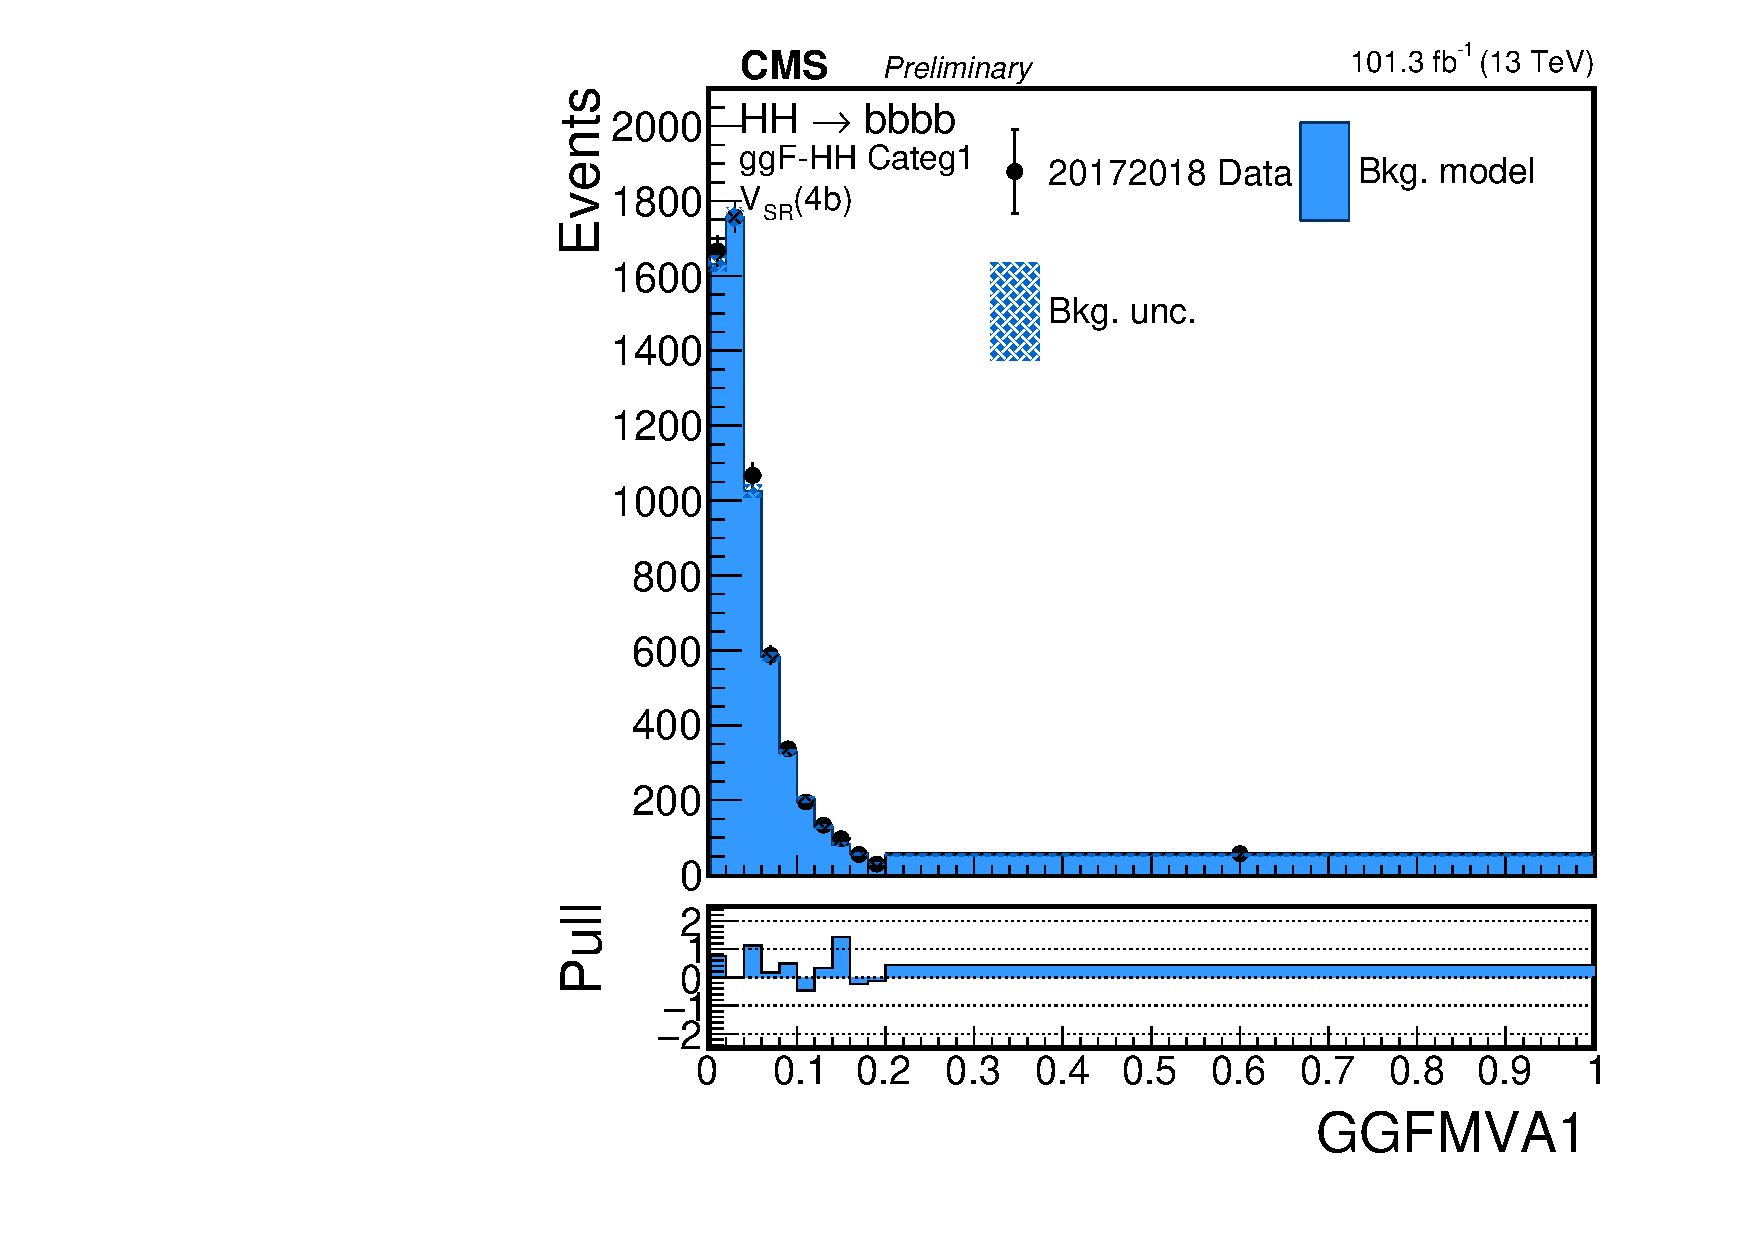
\includegraphics[width=0.48\linewidth]{Figures/Modeling/background/validationobservables/20172018/plot20172018_GGFMVA1_Btag4_GGFcateg1_SR_210_Histogram_postfit.pdf}}
\subfloat[]{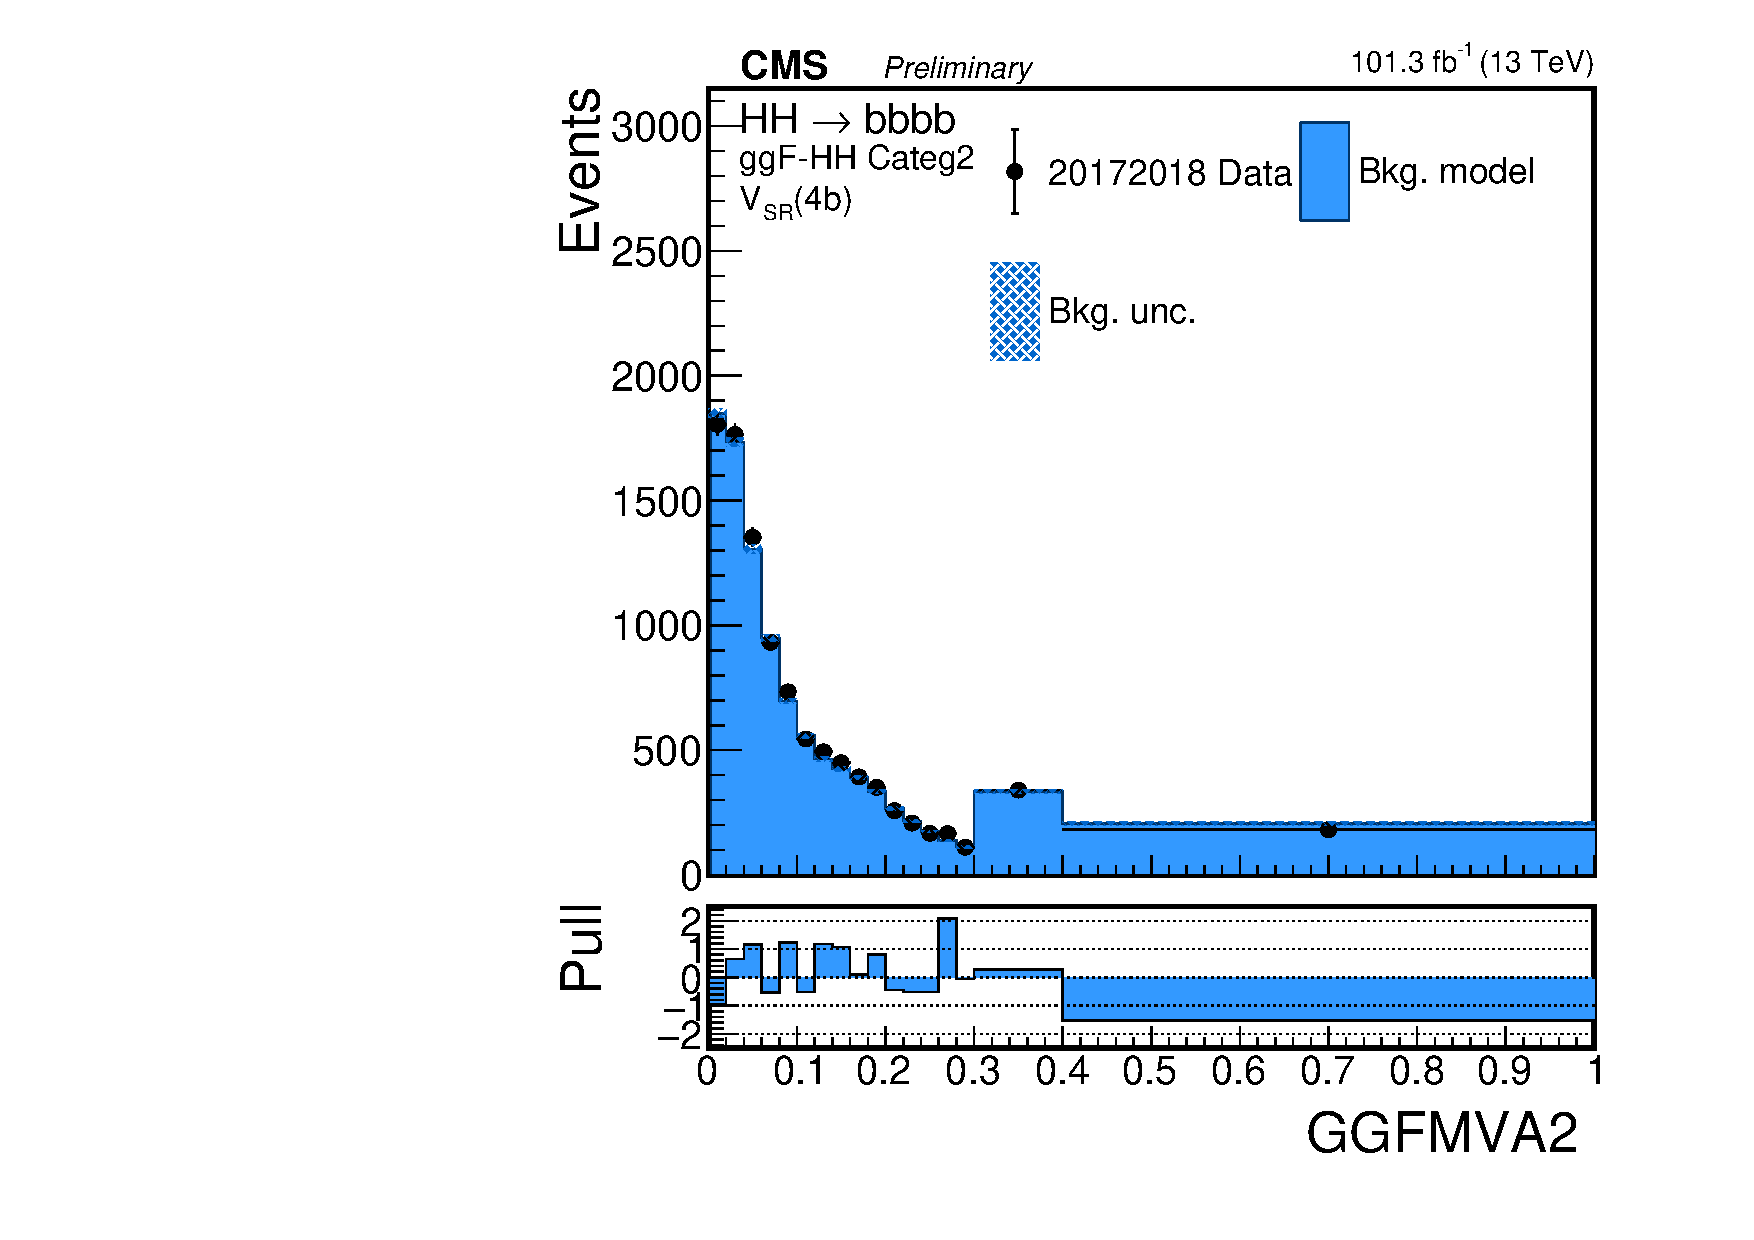
\includegraphics[width=0.48\linewidth]{Figures/Modeling/background/validationobservables/20172018/plot20172018_GGFMVA2_Btag4_GGFcateg2_SR_210_Histogram_postfit.pdf}}\\
\subfloat[]{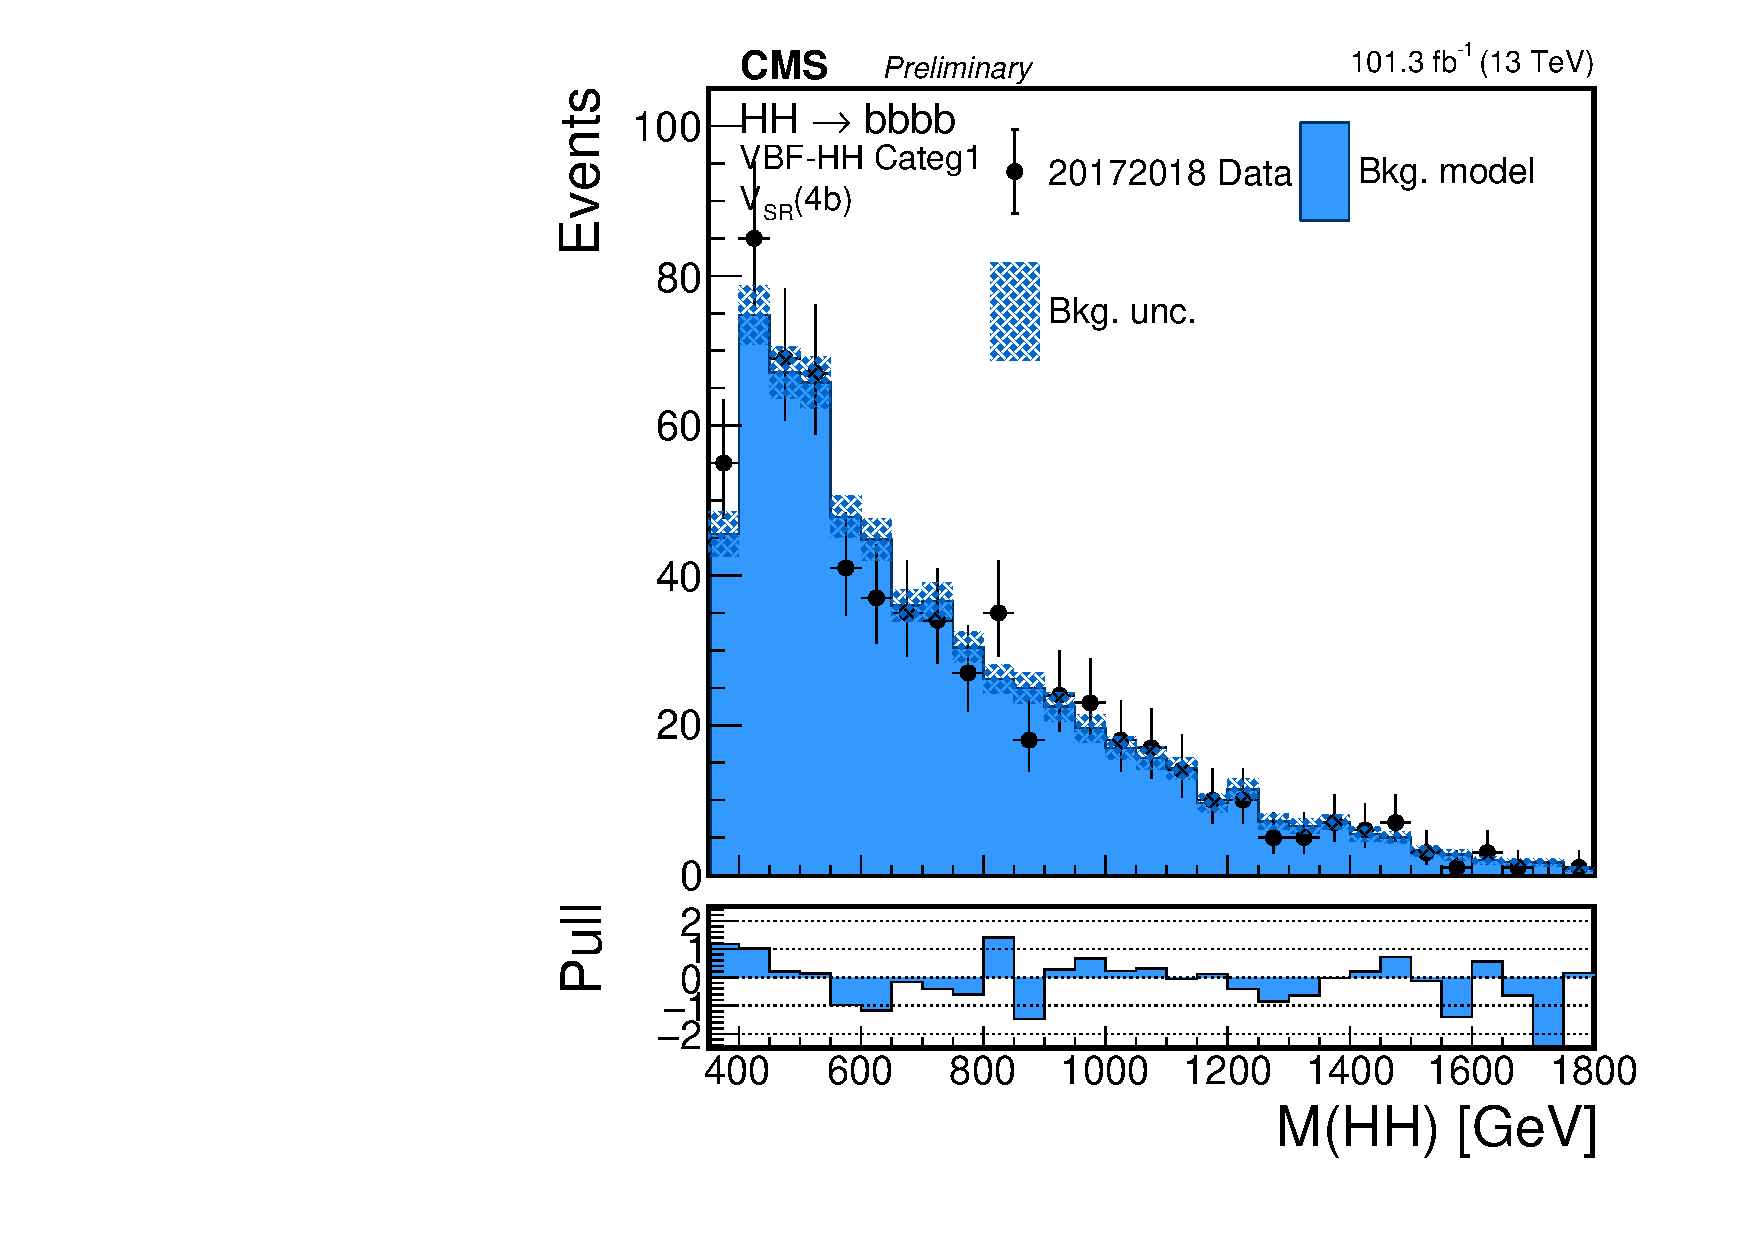
\includegraphics[width=0.48\linewidth]{Figures/Modeling/background/validationobservables/20172018/plot20172018_HH_m_1_Btag4_VBFcateg1_SR_210_Histogram_postfit.pdf}}
\subfloat[]{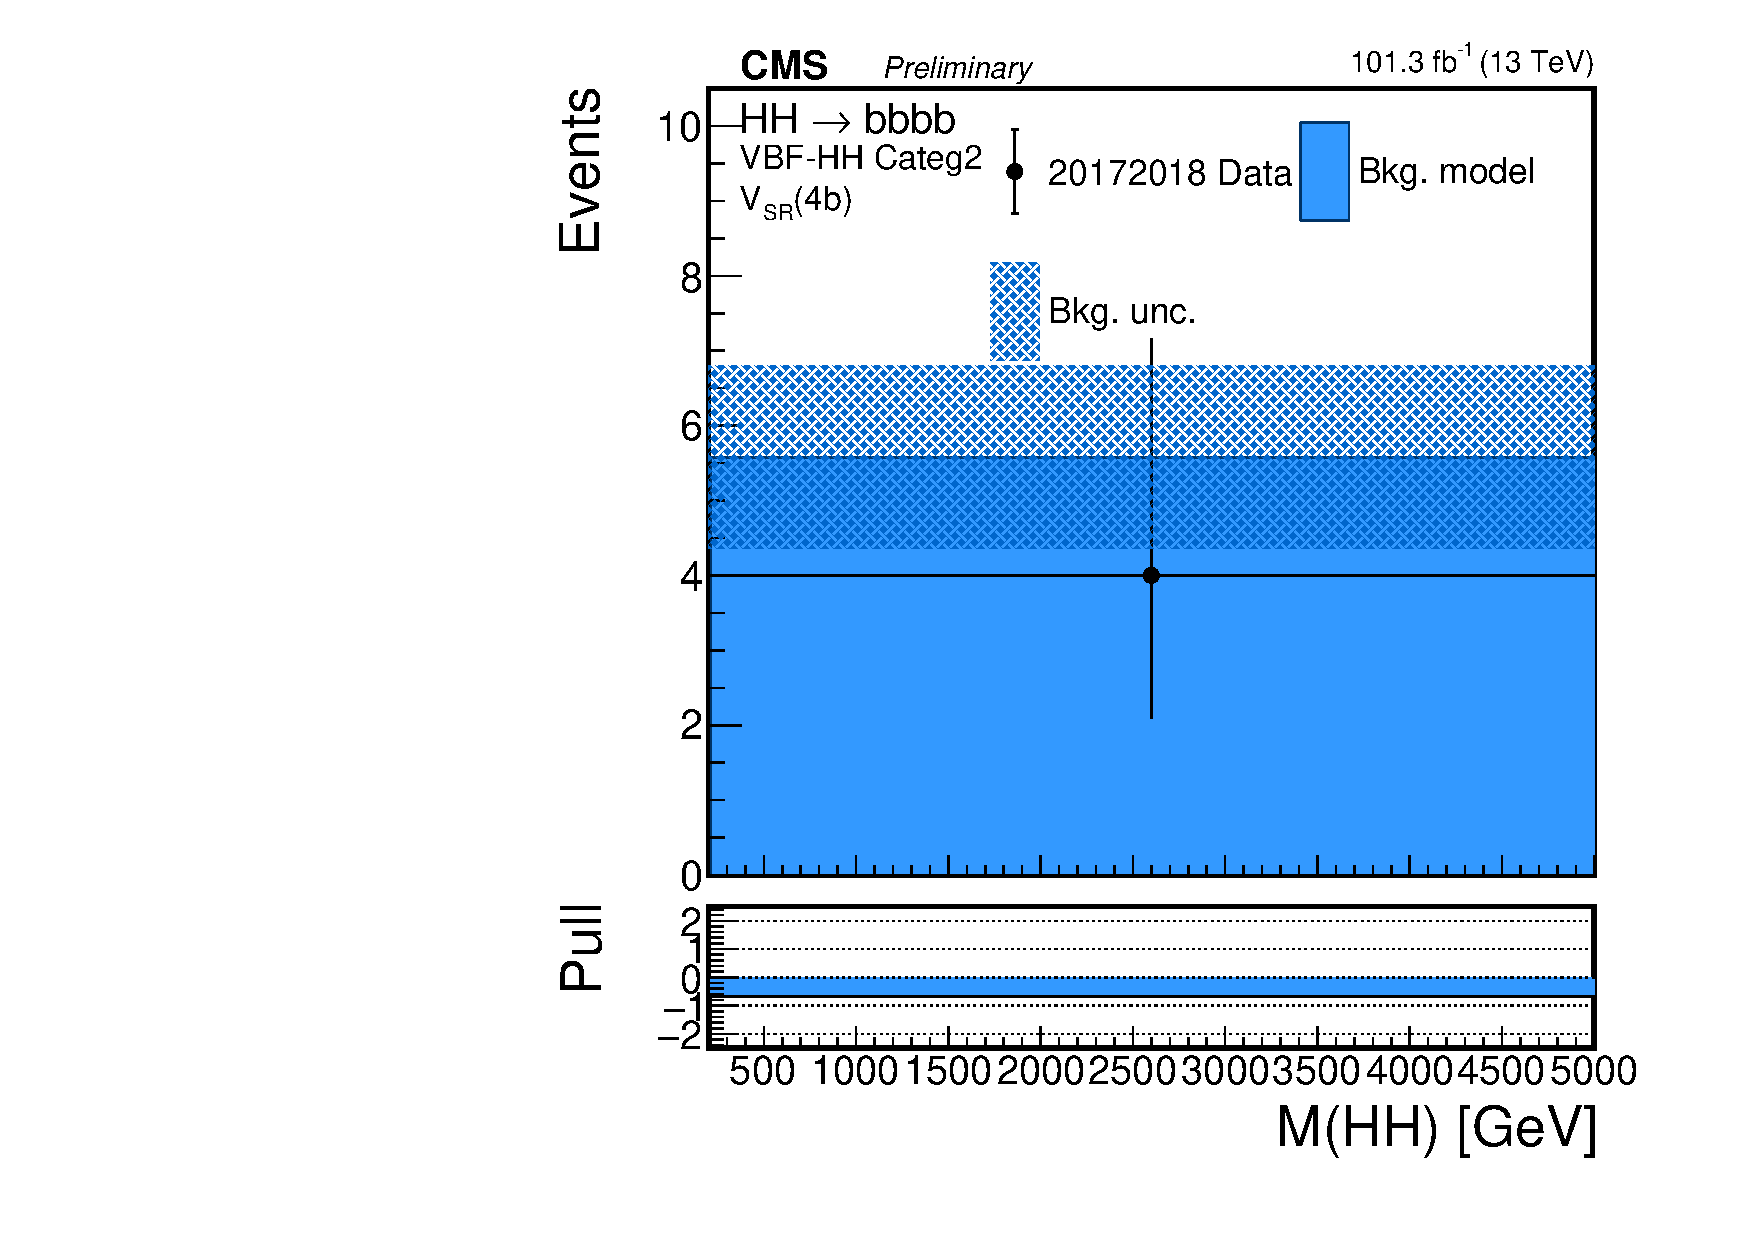
\includegraphics[width=0.48\linewidth]{Figures/Modeling/background/validationobservables/20172018/plot20172018_HH_m_2_Btag4_VBFcateg2_SR_210_Histogram_postfit.pdf}}
\end{center}
\caption[Distributions of the observables in all validation signal regions for 2017-2018 data]{Distributions of the observables in all validation signal regions for 2017-2018 data.  A) ggF category 1, B) ggF category 2, C) VBF category 1, D) VBF Category 2. The presented background distributions are the one obtained after fitting the background prediction to the data floating the background uncertainties.}
\label{fig:bkgobservablesvaltest20172018}
\end{figure}

\clearpage
\subsection{Additional Checks} \label{sec:additionalchecks}
\subsubsection{Self-bias test}

The presence of signal in the 3b regions may impact the modeling of the background. Signal events failing the four b tagging requirement can be assigned to the part of the 3b region used to train the BDT reweighting method and to derive the background model. Given that these events are identified as background, but have the kinematic properties of the HH process, they can mimic the signal signature in the $\mathrm{A_{SR}}$(4b), introducing a bias on the background estimation, and thus reduce the sensitivity of the analysis. 

A signal events classified in the $\mathrm{A_{CR}}$(3b) typically result from an erroneous jet pairing, or from wrongly selection of an additional jet in the event that does not come from the $\hhtobbbb$ process. These events consequently have different properties with respect to the `good' $\mathrm{A_{SR}}$(4b) events because they have similar distributions to the background events in the $\mathrm{A_{SR}}$(3b), and thus have a negligible impact on the training of the background BDT reweighting. However, as events from the $\mathrm{A_{SR}}$(3b) region are used to model the background template, the contamination of HH signal events in that region may introduce a spurious `signal-induced' background component that can mask the actual signal presence in the SR(4b). In order to understand the $\mathrm{A_{SR}}$(3b) signal impact, a `self-bias' test is performed. The test is run with toy experiments using, in each studied subcategory of the analysis separately, the following inputs:
\begin{itemize}
    \item $b_\text{true}$ : The expected distribution of background events in the $\mathrm{A_{SR}}$(4b). It represents the `true' background source
    \item $s$ : The signal distribution in the $\mathrm{A_{SR}}$(4b) region
    \item $b_\text{sig}$ : The distribution of signal events in the $\mathrm{A_{SR}}$(3b) corrected using the exact same transfer model used in the background modeling. It represents the signal events erroneously treated as background.
\end{itemize}

The self-bias test evaluates the bias induced on the best fitted signal strength ($\hat{\mu}$) when a signal of strength $\mu_\text{inj}$ is injected. In essence, this is done in three steps: (1) generate 2000 toys according to $\mu_\text{inj} \cdot s + b_\text{true}$, (2) fit each toy with $\mu \cdot s + \mu_\text{inj} \cdot b_\text{sig} + b_\text{true}$, (3) compare the average and pull of the best fit $\hat{\mu}$ as function of $\mu_\text{inj}$. As a cross-check, the toys are fit with $\mu \cdot s + b_\text{true}$. The test is carried out for values of $\mu_\text{inj}$ up to approximately a factor of 4 times larger than the expected 95\% CL upper limit on the SM ggF and VBF signal strengths obtained in two ggF categories and two VBF categories, respectively. A simple statistical model is used with a log-normal uncertainty of 5\% on $s$, and a log-normal uncertainty of 5\% on $b_\text{true}$ and $b_\text{sig}$. The uncertainties have a negligible impact on the sensitivity, and the test shows the impact of the self-bias with essentially statistical uncertainties only. The bias impact on the full results (that includes systematic uncertainties) is consequently expected to be smaller.

The outcome of the test is illustrated for the 2016 analysis in Figures~\ref{fig:bkg:self-bias-mu} and~\ref{fig:bkg:self-bias-pull}. They report the average value of $\hat{\mu}$ in toys ($<\hat{\mu}>$), and the $<\hat{\mu}>$ pull with respect to $\mu_\text{inj}$ normalized to the 1 standard deviation of the $\hat{\mu}$ distribution ($\sigma_{\hat{\mu}}$). A mild effect of the presence of $b_\text{sig}$ can be observed, but the best-fit signal strength is well compatible within the expected one standard deviation of $\hat{\mu}$ spread, to the one obtained without the $b_\text{sig}$ term in the fit. Therefore, at the current level of sensitivity, the contamination of the signal in the background estimation regions has a negligible impact.

\begin{figure}[ht!]
\captionsetup[subfigure]{justification=centering}
\centering
\subfloat[]{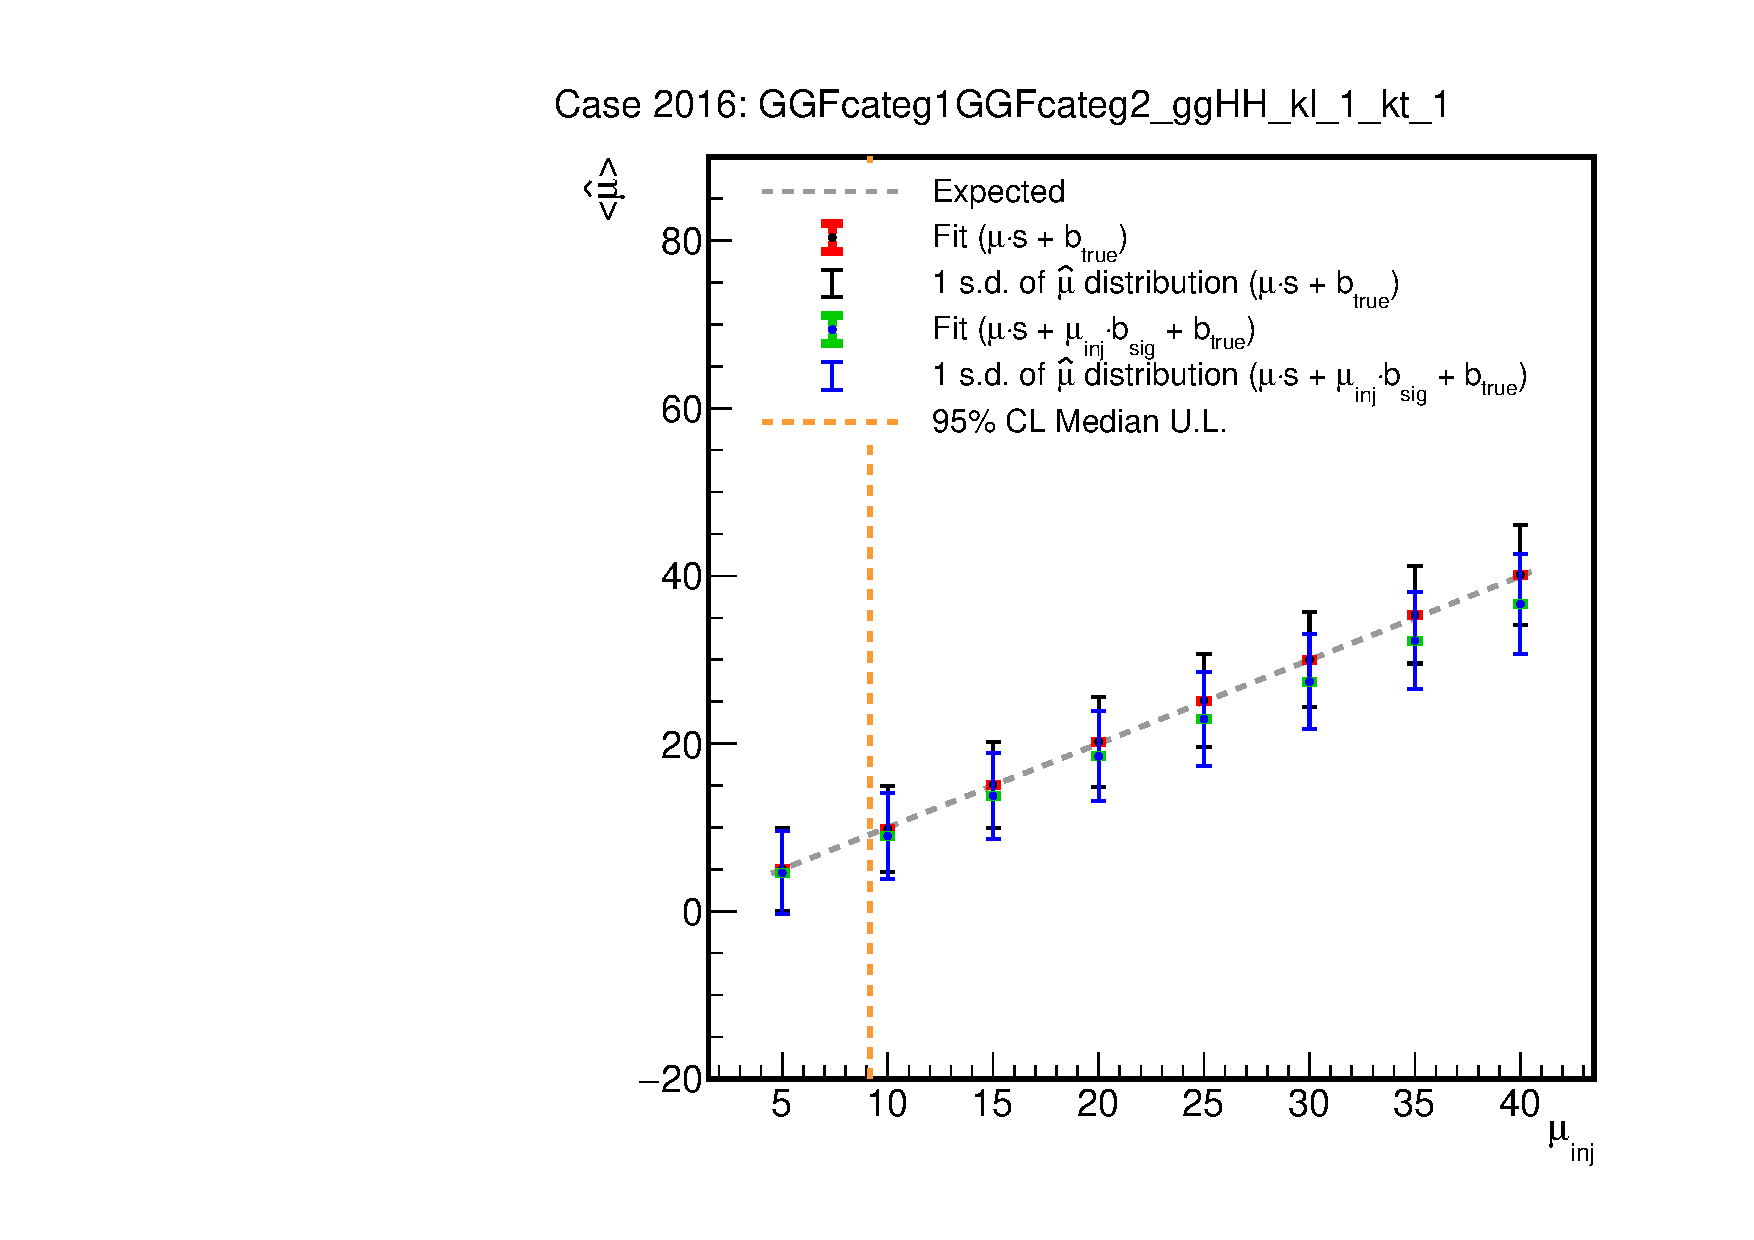
\includegraphics[width=0.40\linewidth]{Figures/Modeling/background/selfbias/tests/2016/selfbiasmodel2016_GGFcateg1GGFcateg2_ggHH_kl_1_kt_1_bestfit_both.pdf}}
\subfloat[]{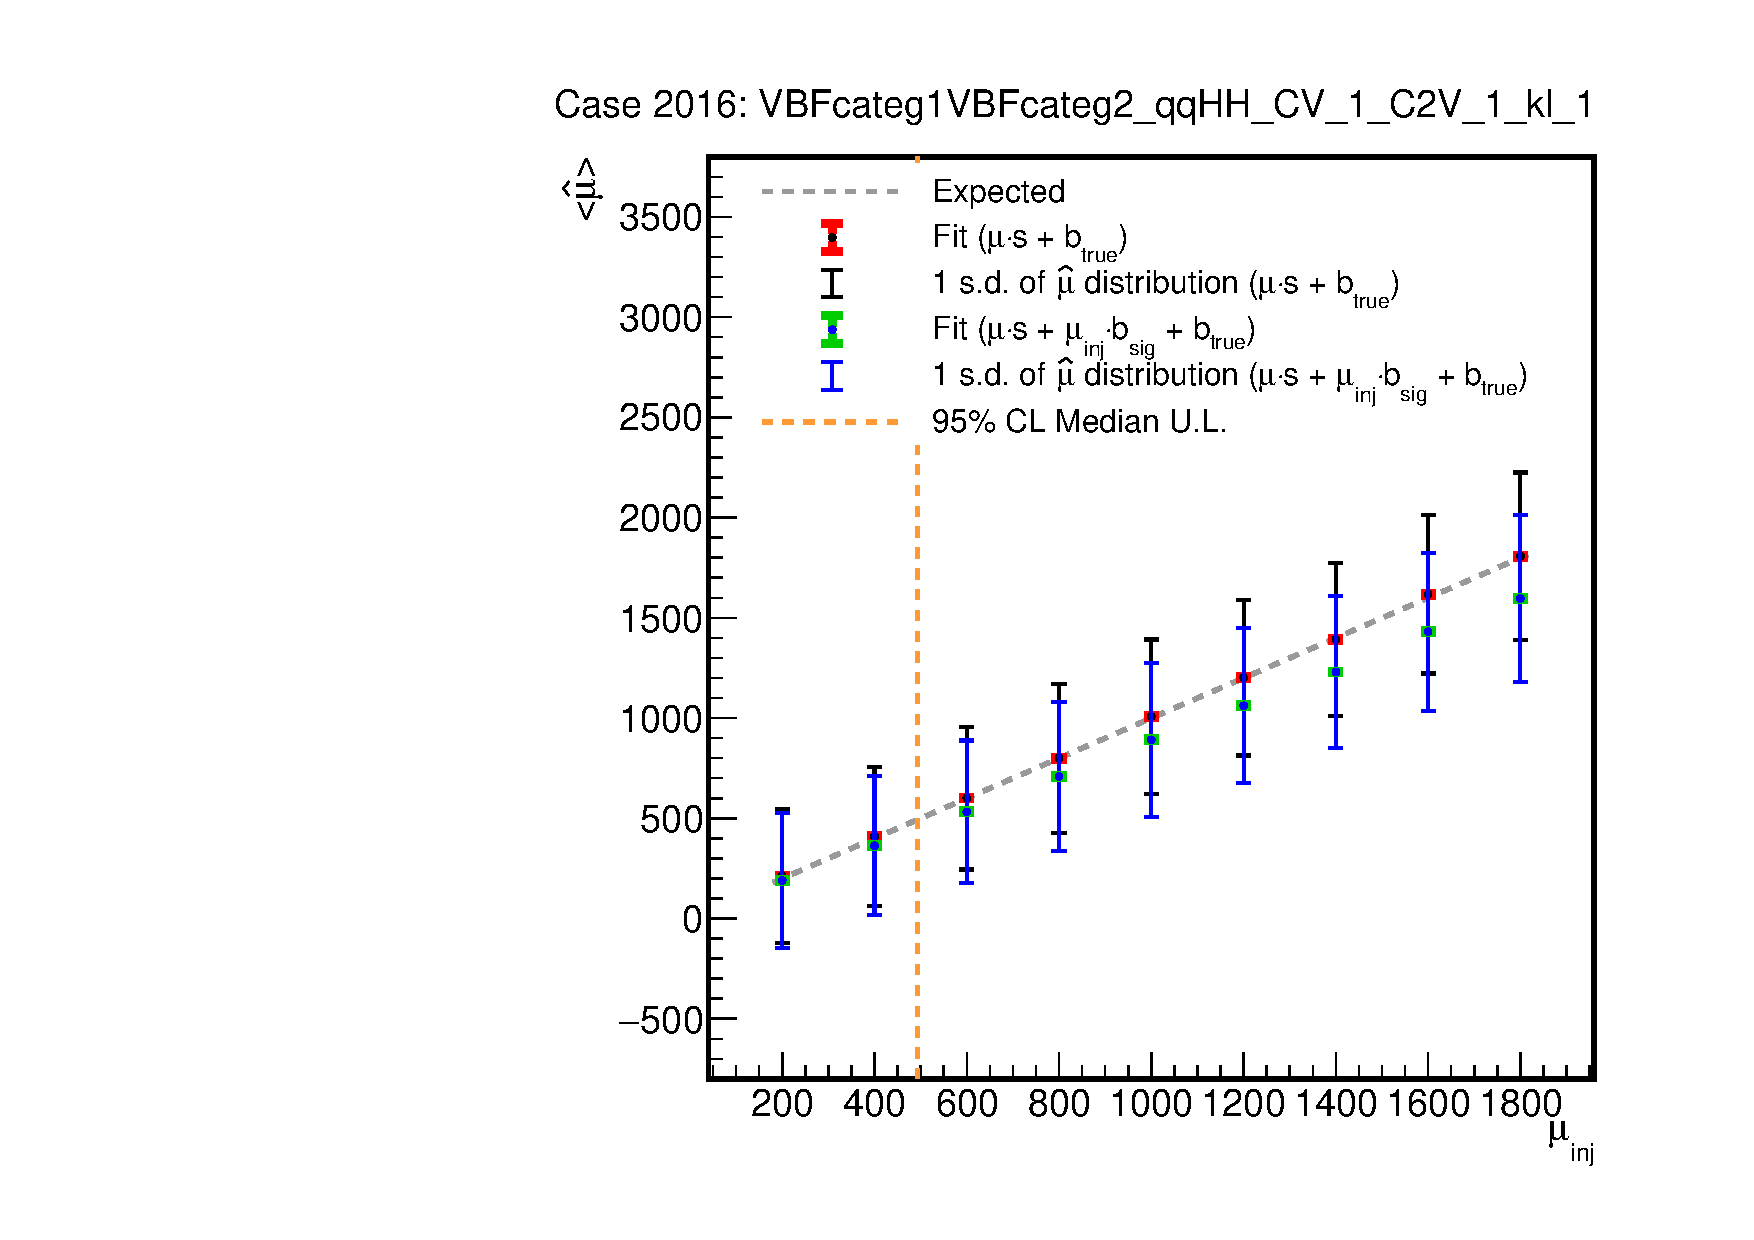
\includegraphics[width=0.40\linewidth]{Figures/Modeling/background/selfbias/tests/2016/selfbiasmodel2016_VBFcateg1VBFcateg2_qqHH_CV_1_C2V_1_kl_1_bestfit_both.pdf}}\\
\caption[Example of the self-bias impact on fitted signal strength]{Example of the self-bias impact on fitted signal strength. A) ggF signal in the 2016 ggF categories and B) VBF signal in the 2016 VBF categories. The green (red) points and blue (black) error-bars show the average and one standard deviation of the best fit signal strength $\hat{\mu}$ distribution when the fit is performed under the model with (without) the self-bias term $b_\text{sig}$. The vertical line denotes the 95\% CL upper limit in that category.}
\label{fig:bkg:self-bias-mu}
\end{figure}

\begin{figure}[ht!]
\captionsetup[subfigure]{justification=centering}
\centering
\subfloat[]{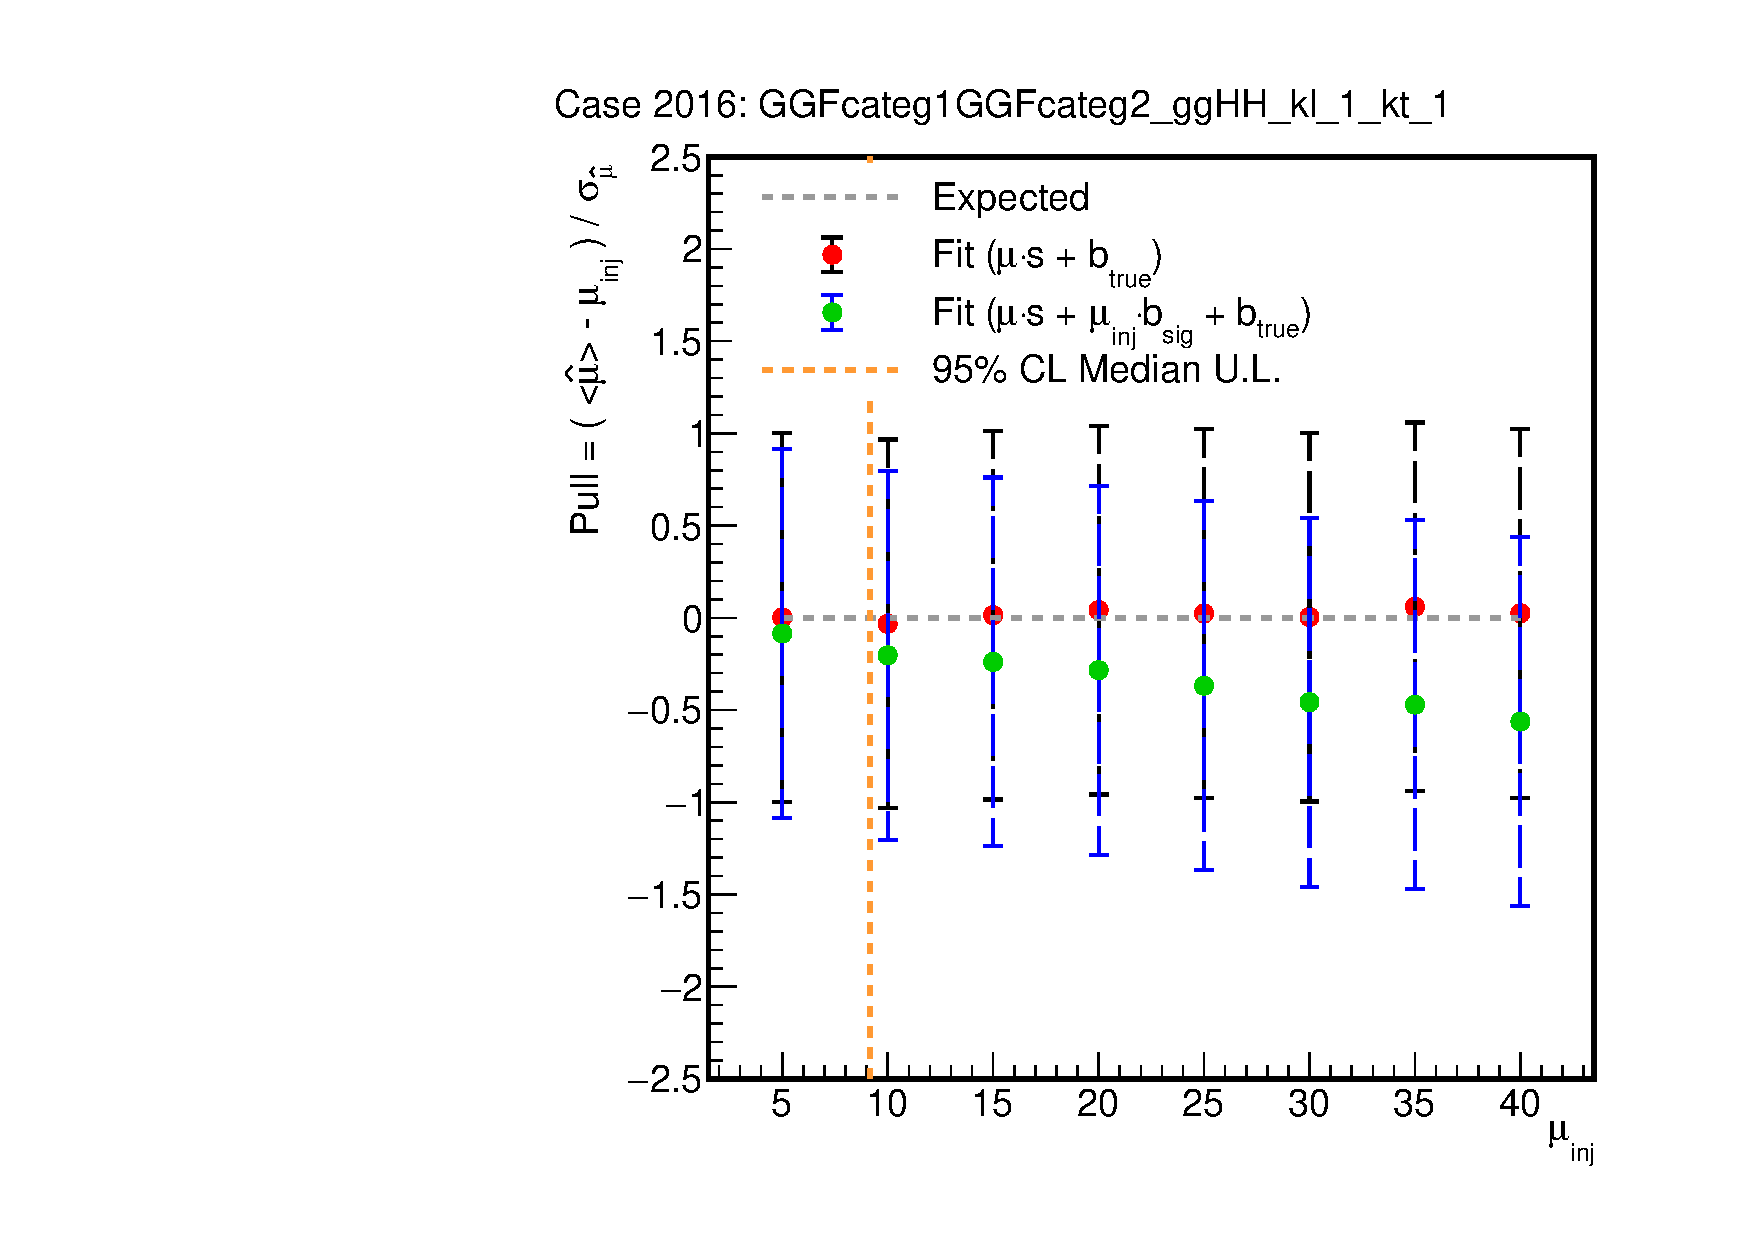
\includegraphics[width=0.40\linewidth]{Figures/Modeling/background/selfbias/tests/2016/selfbiasmodel2016_GGFcateg1GGFcateg2_ggHH_kl_1_kt_1_pull_both.pdf}}
\subfloat[]{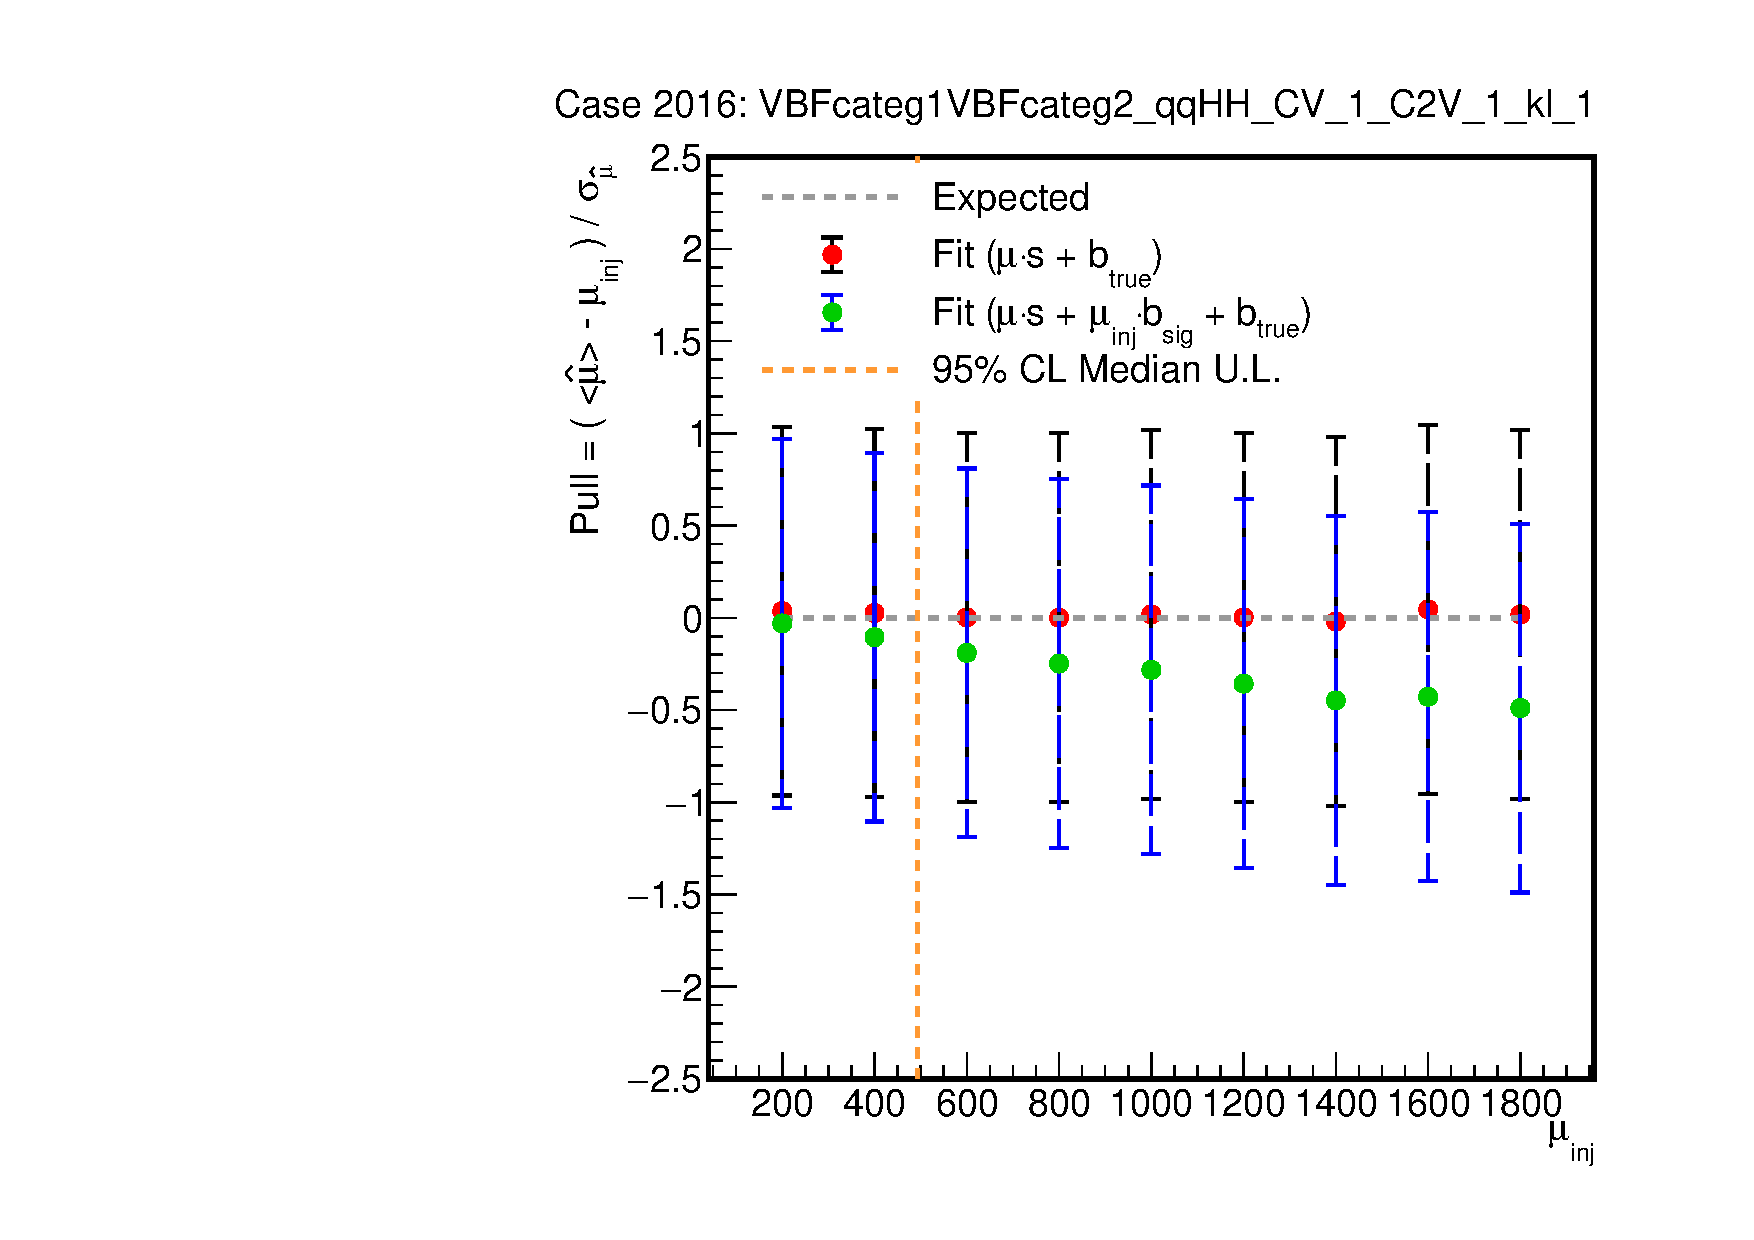
\includegraphics[width=0.40\linewidth]{Figures/Modeling/background/selfbias/tests/2016/selfbiasmodel2016_VBFcateg1VBFcateg2_qqHH_CV_1_C2V_1_kl_1_pull_both.pdf}}\\
\caption[Example of the self-bias impact on the fitted signal strength pull]{Example of the self-bias impact on the fitted signal strength pull. A) ggF signal in the 2016 ggF categories and B) VBF signal in the 2016 VBF categories. The points show the pull of the average of the best fit signal strength $\hat{\mu}$ distribution with respect to the injected signal strength $\mu_\text{inj}$, normalized to one standard deviation of the $\hat{\mu}$ distribution. The fit is performed under the model with (without) the self-bias term $b_\text{sig}$ and shown in green (red). The vertical line denotes the 95\% CL upper limit in that category.}
\label{fig:bkg:self-bias-pull}
\end{figure}

\subsubsection{Single Higgs impact}
The dominant single Higgs contribution comes from $\ttbarh$($\mathrm{b\overline{b}}$) events (65\%-95\% of the total single H depending on the category and year). The contribution of single Higgs production to the background events is assumed to be covered by the background model. This hypothesis is studied using $\ttbarh$($\mathrm{b\overline{b}}$) events in the $\mathrm{A_{SR}}$(4b) region observables of the ggF categories in 2016 and 2017+2018. 

The study evaluates the expected distribution of $\ttbarh$($\mathrm{b\overline{b}}$) events, and how much of it is covered by our background model. The expected coverage is evaluated by transforming $\ttbarh$($\mathrm{b\overline{b}}$) in the $\mathrm{A_{SR}}$(3b) region with the background model method, here denominated as the `$\ttbarh$(bb) model'. The results are presented in Figure~\ref{fig:bkg:tthimpact}. The signal region distributions correspond to the background model statistical uncertainty (in blue), expected $\ttbarh$($\mathrm{b\overline{b}}$) events (in green), expected `ttH(bb) model' (in orange), and the expected SM-HH signal scaled by expected upper limit (in red). 

The outcome shows that the background estimate models partially the expected $\ttbarh$($\mathrm{b\overline{b}}$) events. This effect is expected since we do not expect the method to learn to model $\ttbarh$($\mathrm{b\overline{b}}$) in the CR because most of the $\ttbarh$ background will be in the SR given the resonant H($\mathrm{b\overline{b}}$) signature. However, this is not a concern because this contribution is overshadowed by the statistical uncertainty of the background estimate.

\begin{figure}[ht!]
\captionsetup[subfigure]{justification=centering}
\centering
\subfloat[]{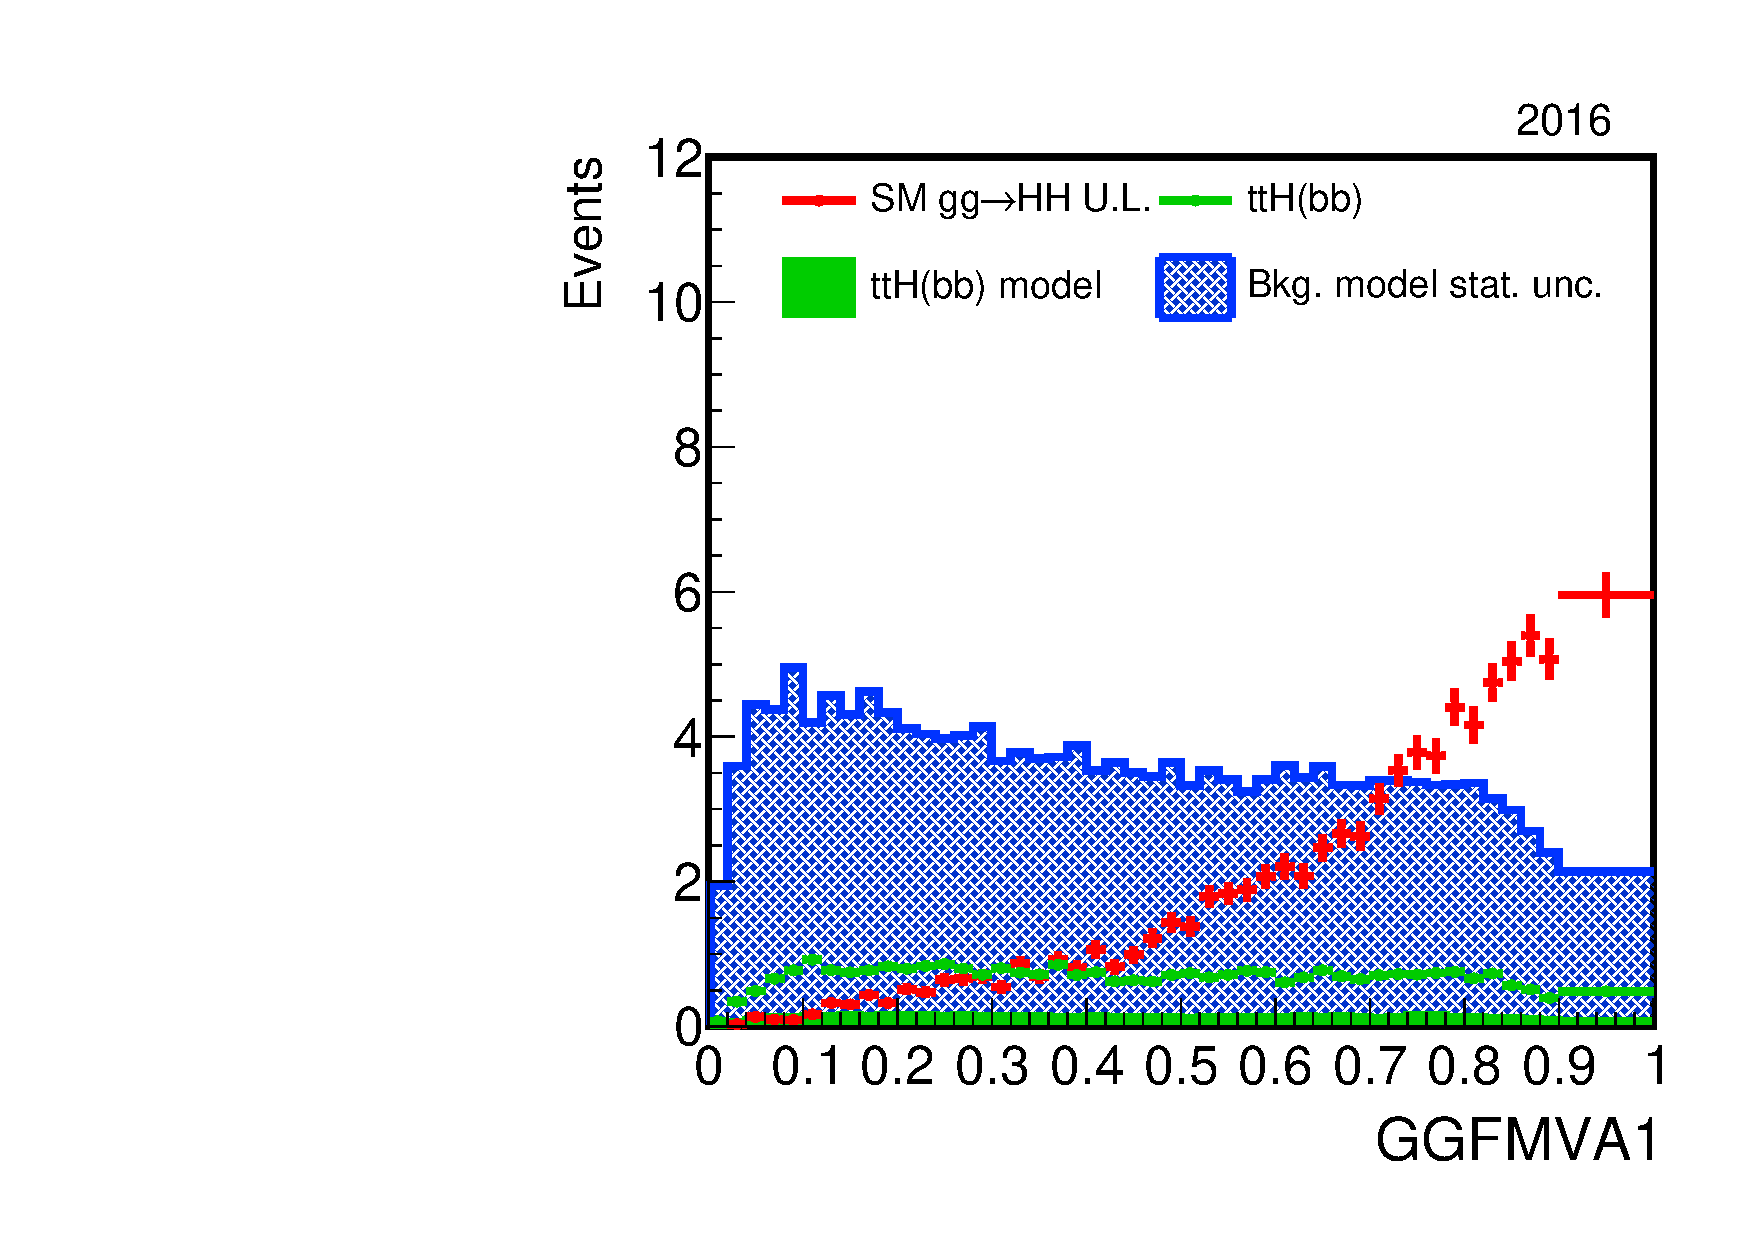
\includegraphics[width=0.45\linewidth]{Figures/Modeling/background/tthtest/2016/plot_datamodel_h_GGFMVA1.pdf}}
\subfloat[]{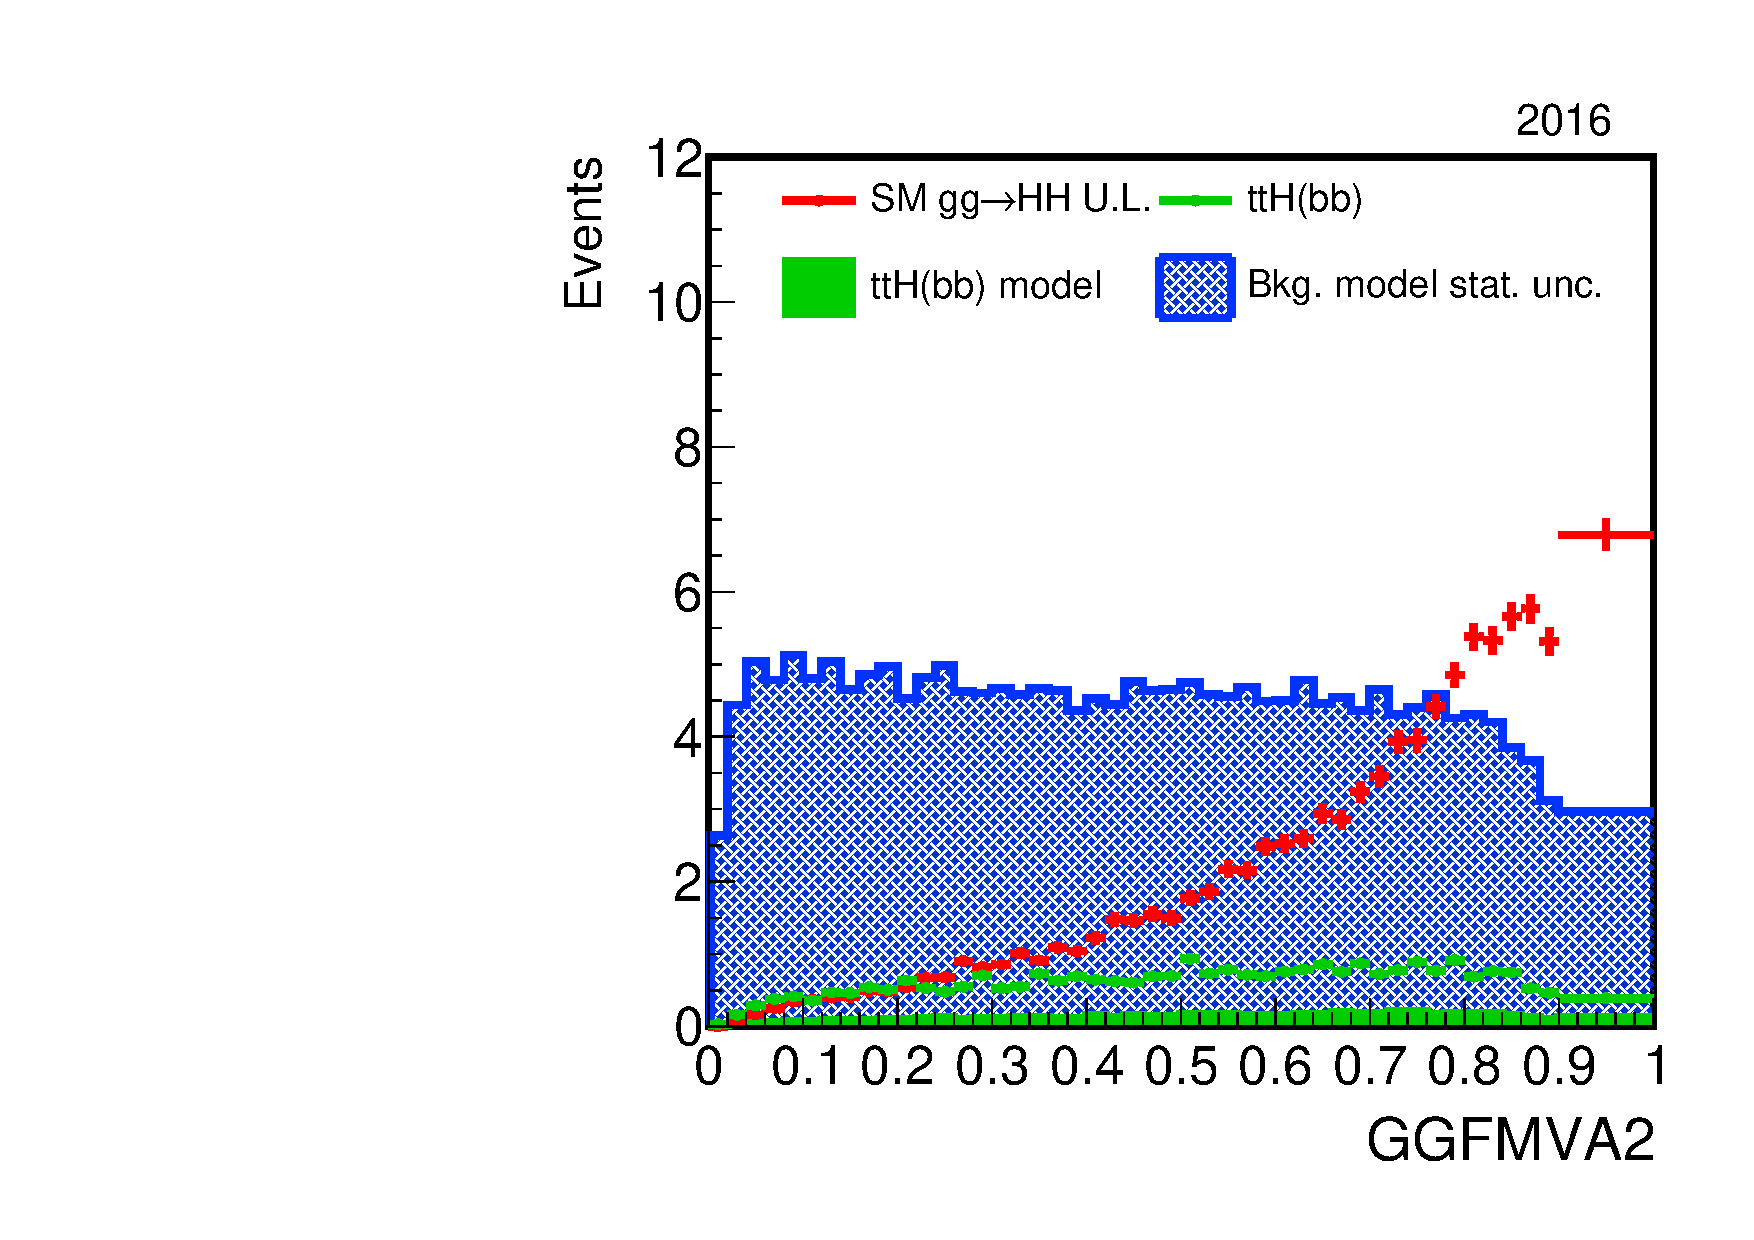
\includegraphics[width=0.45\linewidth]{Figures/Modeling/background/tthtest/2016/plot_datamodel_h_GGFMVA2.pdf}}\\
\subfloat[]{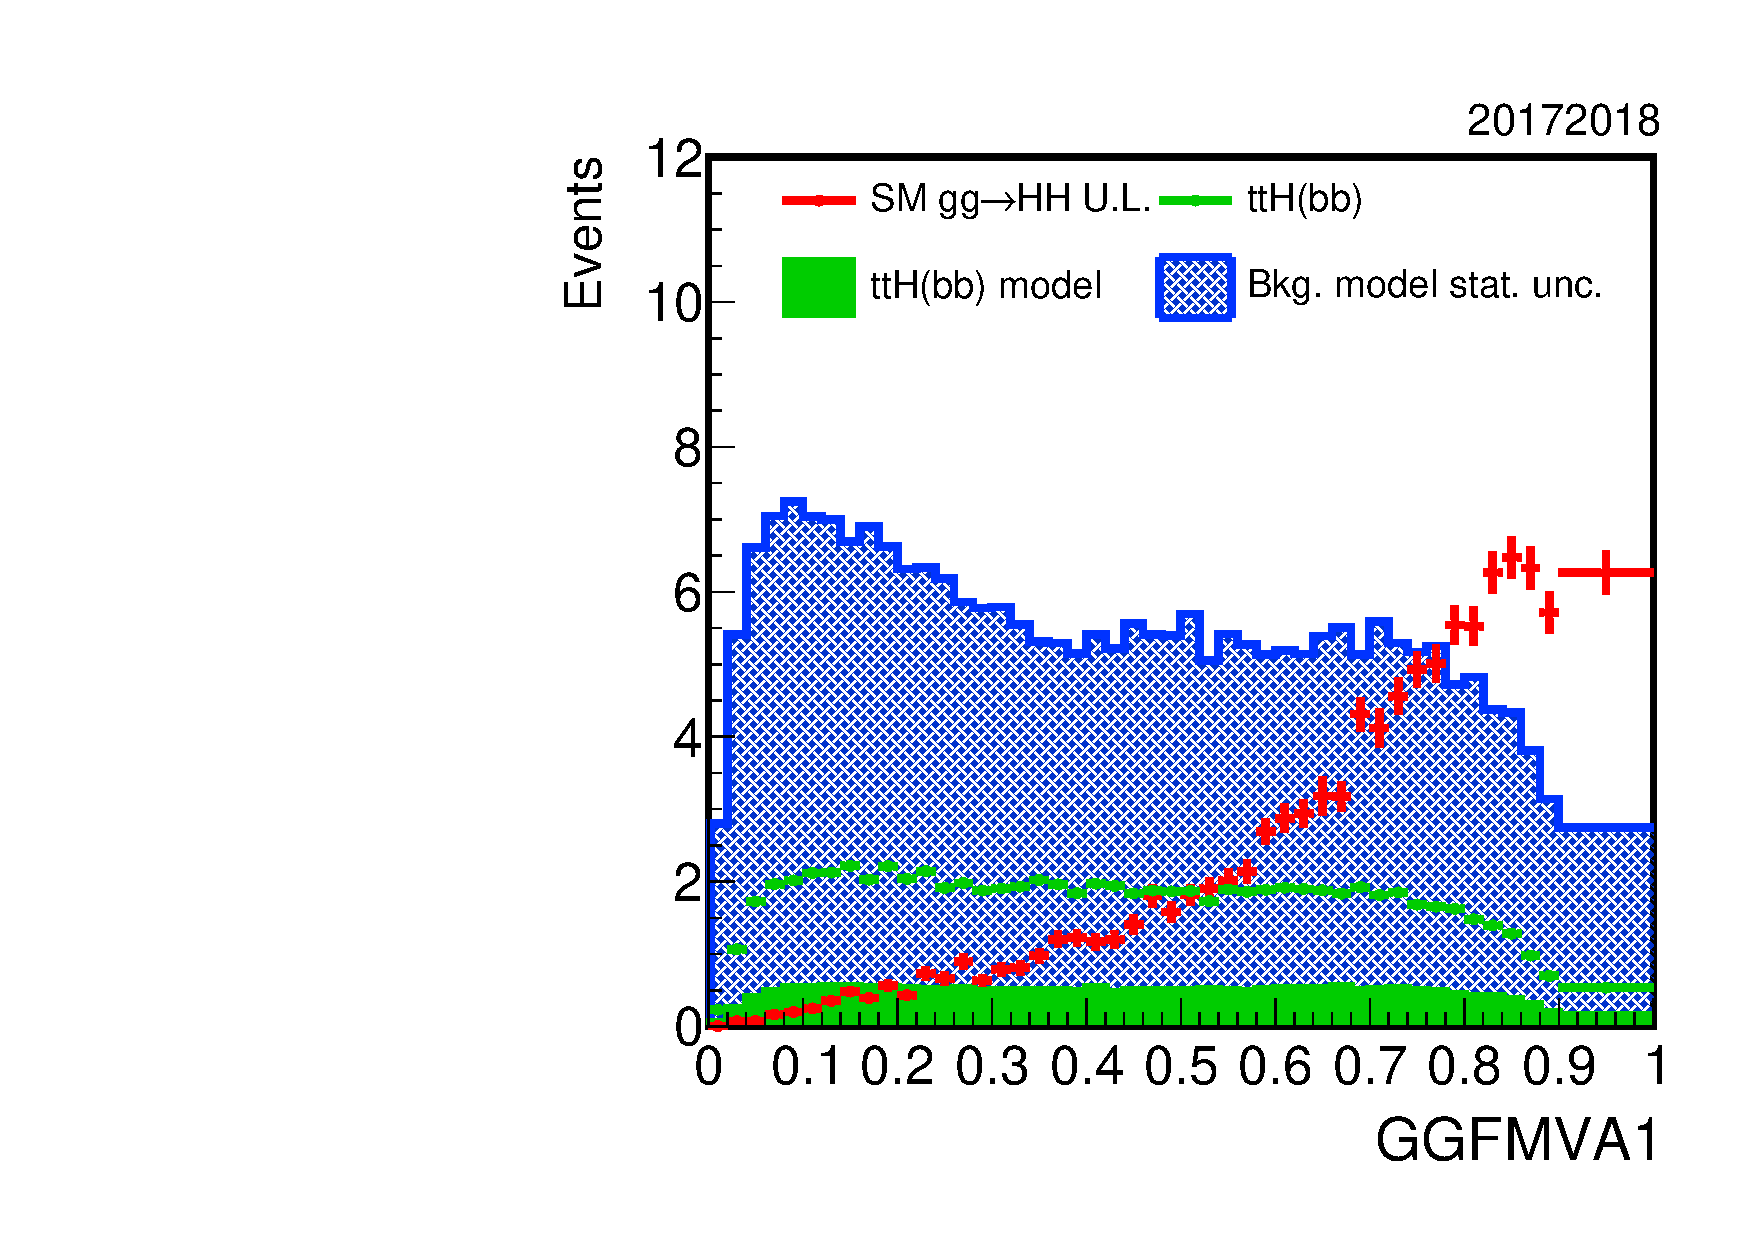
\includegraphics[width=0.45\linewidth]{Figures/Modeling/background/tthtest/20172018/plot_datamodel_h_GGFMVA1.pdf}}
\subfloat[]{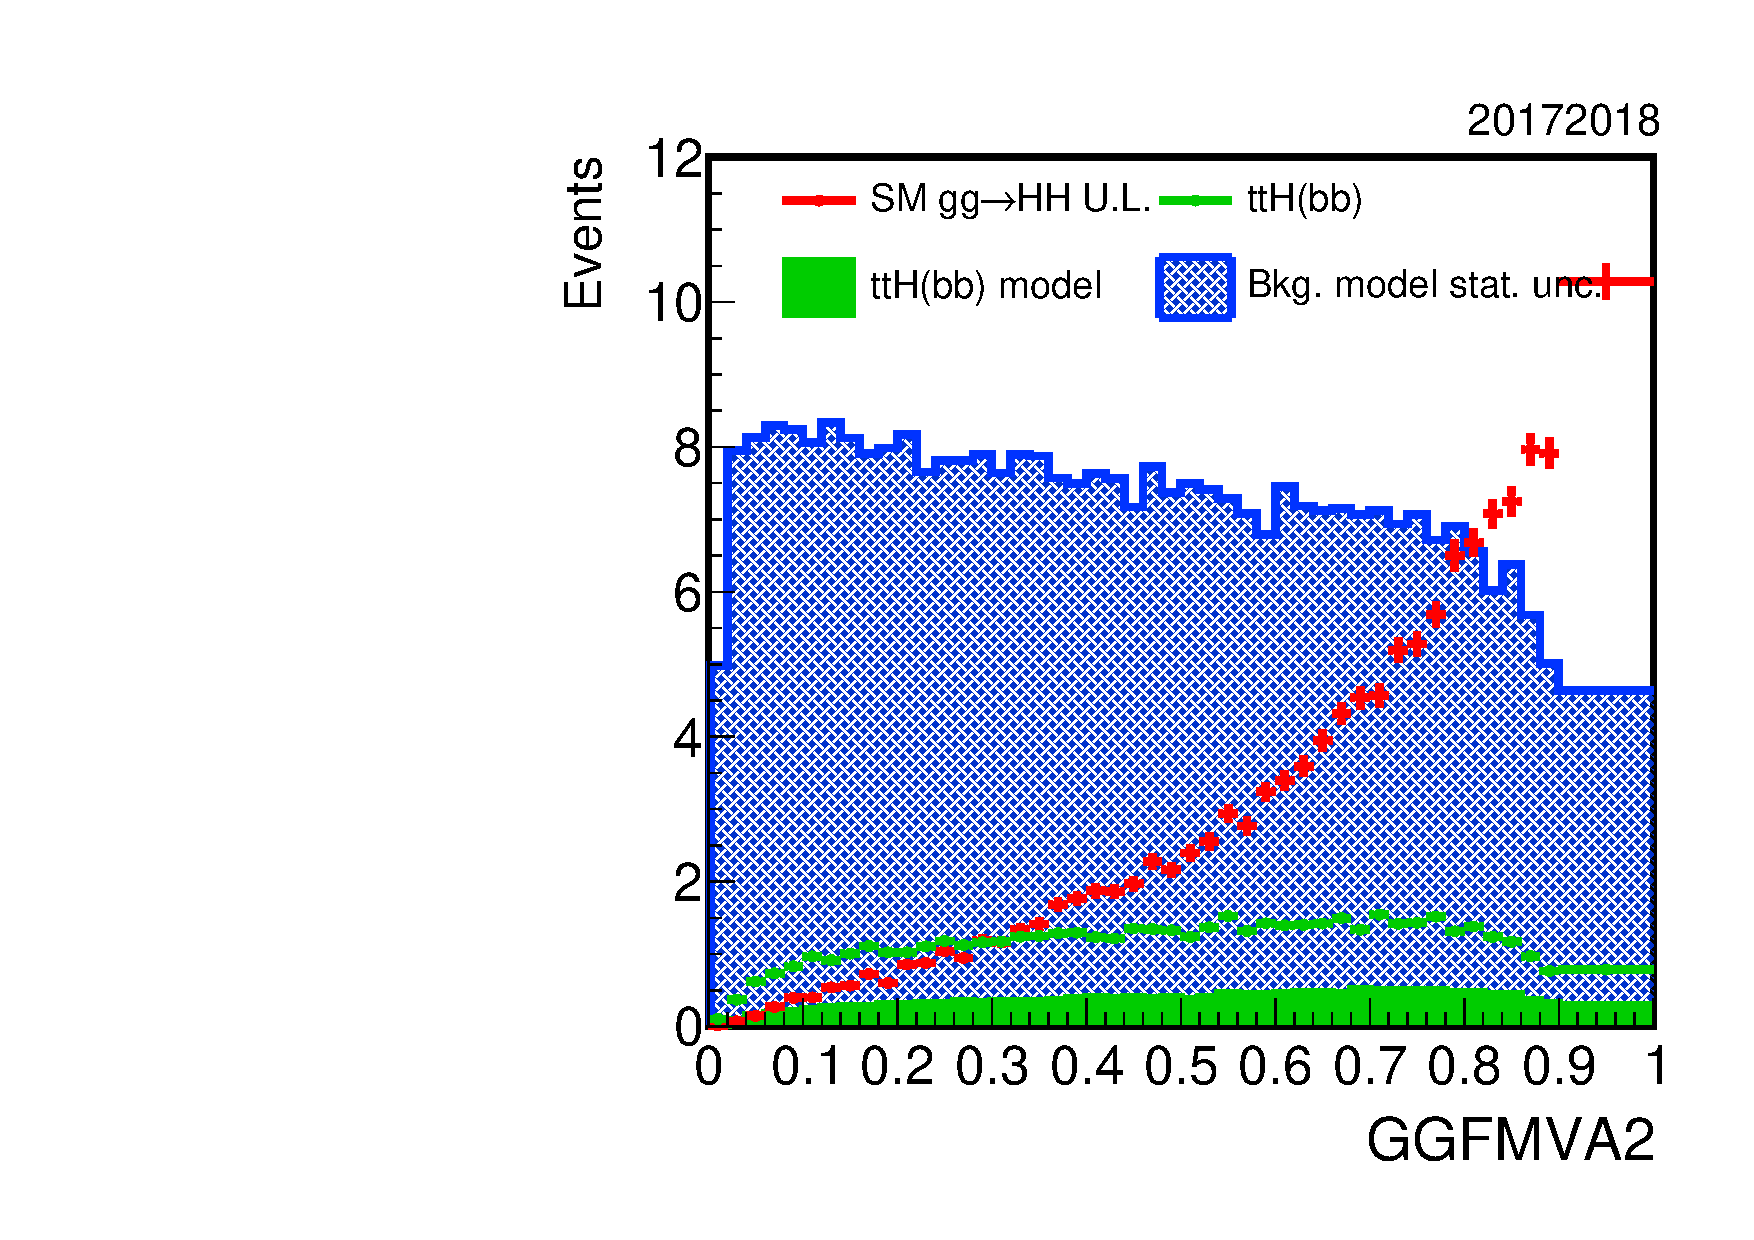
\includegraphics[width=0.45\linewidth]{Figures/Modeling/background/tthtest/20172018/plot_datamodel_h_GGFMVA2.pdf}}\\
\caption[Impact of the Higgs boson production with associate top-quark pairs in the four observables of the ggF $\mathrm{A_{SR}}$(4b) regions]{Impact of the Higgs boson production with associate top-quark pairs in the four observables of the ggF $\mathrm{A_{SR}}$(4b) regions. A) ggF category 1 in 2016, B) ggF category 2 in 2016, C) ggF category 1 in 2017-2018, D) ggF category 2 in 2017-2018.  } 
\label{fig:bkg:tthimpact}
\end{figure}

\section{Systematic Uncertainties} \label{systematics}
\subsection{Signal Uncertainties} \label{sigsystematics}
The modeling of the signal yields and shape can be affected by sources of uncertainty associated to experimental measurements, event generation, and theoretical predictions. These systematic uncertainties are evaluated in all signals (6 ggF, 3 VBF, 12 EFT nodes) for the 2016, 2017 and 2018 simulation campaigns. The following sources are considered:
\begin{itemize}
    \item {Luminosity:} As the signal yields are normalized according to the measured integrated luminosity, a normalization uncertainty is assigned to account for the uncertainty from the CMS luminosity measurements. The amounts are 1.2\% for 2016~\cite{CMS-LUM-17-003}, 2.3\% for 2017~\cite{CMS-PAS-LUM-17-004}, and 2.5\% for 2018~\cite{CMS-PAS-LUM-18-002}.
    \item {Pileup reweighting:} A normalization uncertainty is derived with an alternative reweighting of the number of pileup interaction. This alternative reweighting is made by shifting the minimum bias cross section by 4.6\%.
    \item {b-tagging algorithm:} 
    Difference between data and simulation on the performance of the deepJet algorithm are addressed using scale factors provided by the CMS BTAG POG. Then, their impact on the signal modeling is evaluated by varying these factors within their uncertainties and propagating the effect in the analysis.
    \item {Trigger:} The efficiency of the simulated triggers is corrected to match the one measured in data using a correction scale factor using the procedure described in Section~\ref{sec:trigger}. The uncertainty on this procedure is derived by varying the factor within its uncertainties and propagating them on the full data analysis.
    \item {Jet energy scale (JES):} There are a total of 21 uncertainty sources in the jet energy scale, which are at the order of few percent and depend on $\pt$ and $\eta$. The analysis uses the `reduced' set recommended by the CMS JETMET POG, which roughly groups them by detector regions into a total of 11 sources. The impact of each uncertainty on the signal yield is calculated independently by varying the jet energy scale within the recommended uncertainties and rerunning the full analysis selection. 
    \item {Jet energy resolution (JER):} The uncertainty on the jet energy resolution is taken into account by varying the jet resolution within the recommended uncertainties, and rerunning the full analysis selection. This uncertainty is considered as a signal shape uncertainty.
    \item {Level-1 Prefiring:} A gradual shift in the timing of the ECAL L1 trigger inputs at the forward region was observed during the 2016 and 2017 operations. This led to decrease of efficiency for events with a significant amount of ECAL energy in the $2<|\eta|<3$ region. This effect is not simulated by default. and thus, correction factors and uncertainties were provided by trigger experts to account for it. Then, a signal normalization uncertainty associated to these corrections is derived by varying them within their uncertainties and propagating them to the final result.
    \item {Event generator:} The impact of the normalization and renormalization scales in the event generation are addressed by first propagating their corresponding variations (implemented as event-by-event weights) in the analysis. Then, the variations are combined by taking the envelope of them, and use the uncertainty.
    \item {PDF:} The uncertainty associated to the choice of PDF is addressed using variations of the PDF weights.
    \item {Hadronization:} Variations of the parton shower weights are used to assign an uncertainty on the modeling of the parton shower. For this purpose, the uncertainty is derived by combining four variations in quadrature.
    \item {ISR recoil scheme} The uncertainties in the modeling of additional radiation in VBF topologies is estimated by comparing samples generated with the \texttt{dipoleRecoil} PYTHIA option turned on and off. Nominal samples are generated without \texttt{dipoleRecoil} since this option was not yet available for the 2016 MC campaign. The difference in the yields of the VBF signals simulated with and without this option is considered as a systematic uncertainty, and the effect observed is a change in the sharing of the signal in the ggF and VBF categories corresponding to an uncertainty of 10-15\% depending on the year and category considered. For the 2016 simulation, where no \texttt{dipoleRecoil} exists, the largest uncertainty between 2017 and 2018 is used.
    \item {Theoretical HH cross section:} These uncertainties correspond to $+2.2\%/-5.0\%$ (scale), $\pm 3\%$ (PDF), and $\pm 2.6\%$ ($m_{t}$) for ggF production, and to $+0.03\%/-0.04\%$ (scale) and $\pm 2.1\%$ (PDF + $\alpha_\text{S}$) for VBF production. They are included only when quoting the limit with respect to the SM (i.e. signal strength $\mu$) and for the likelihood scans, and not for the cross section upper limit. For anomalous $\kl$ values, a $\kl$-dependent uncertainty is used following the LHC HH group recommendations. Note: a new recommendation for the ggF uncertainty was published by the LHC HH group after these analysis results were released as a PAS~\cite{thesispas}, thus these are not accounted for in this dissertation.
    \item {Final state branching fraction:} The uncertainty is $\pm 2.5\%$, as obtained by propagating the theoretical uncertainty in the branching ratio of the $\hbb$ decay, assuming $\mathcal{B}(\hbb) = 0.5824 \pm 0.65\% (\text{theory}) {}^{+0.72\%}_{-0.74\%} (m_{b}) {}^{+0.78\%}_{-0.80\%} (\alpha_\text{S})$ for $m_{H} = 125$ GeV~\cite{HiggsBRTwiki}. It is included only when quoting the cross section limit with respect to the SM (i.e. signal strength $\mu$) and for the likelihood scans, but not for the cross section upper limit.    
\end{itemize}
\subsection{Background Model Uncertainties} \label{bkgsystematics}
For the data-driven background model, a dedicated set of systematic uncertainties are considered to account for different effects that impact the predicted normalization and shape of the background templates. These uncertainties are summarized in Tables~\ref{syst:bkg2016} and~\ref{syst:bkg20172018}. They are treated uncorrelated across categories and datasets. The following sources are considered:
\begin{itemize}
    \item {Bin-by-bin:} These uncertainties account for the limited number of events available in the $\mathrm{A_{SR}}$(3b) region. They are the bin-by-bin statistical uncertainty of the $\mathrm{A_{SR}}$(3b) region propagated into the $\mathrm{A_{SR}}$(4b) region. The Barlow-Beeston-lite approach is used~\cite{Barlow:1993dm}.   
    \item {Transfer factor:} The $\mathrm{A_{CR}}$(3b) and $\mathrm{A_{CR}}$(4b) have limited number of events. This impacts the measurement of the transfer factor used to compute the $\mathrm{A_{SR}}$(4b) predicted normalization. A normalization uncertainty is assigned to account for this effect in all categories, as presented in Tables \ref{bkg:tab:factor1} and \ref{bkg:tab:factor2}.
    \item {Validation normalization:} A normalization uncertainty to account for the residual differences between the observed data and background normalization in some categories (up to 2 standard deviations) in the validation studies, presented in Table~\ref{bkg:tab:valfactor1} and Table~\ref{bkg:tab:valfactor2}. The uncertainty is calculated by adding the extra contribution to the total normalization uncertainty that reduces the discrepancy with data to one standard deviation level. 
    \item {Validation statistical precision:} From background validation studies, we observed a very good compatibility between the data and the model across all categories and years in the $\mathrm{V_{SR}}$(4b) region. To validate this procedure, the $\mathrm{V_{SR}}$(4b) region should have a comparable statistical precision with respect to the $\mathrm{A_{SR}}$(4b) region. The statistical precision is defined as $p=1/\sqrt{N_{pred} }$, where $N_{pred}$ is the predicted background normalization. An extra normalization uncertainty is assigned to the categories with $p(A_{SR}^{4b})<p(V_{SR}^{4b})$ using the following formula: $\sigma_{val}=\sqrt{ p(V_{SR}^{4b})^{2} - p(A_{SR}^{4b})^{2}}$.
    \item {Shape:} For the two ggF categories, the reweighing of the observables has a small dependency on the definition of the $\mathrm{A_{CR}}$ region (where the BDT reweighting method is trained). A shape uncertainty is derived to account for this effect by deriving alternative templates in restricted portions of the default $\mathrm{A_{CR}}$ region. The portions used for the alternative trainings are illustrated in Figure~\ref{fig:syst:bkgshaperegions}. Since the kinematic properties of the events are highly correlated with $m_{paral}$, the comparison of the trainings between regions A and B allows for estimating the quality of a training that interpolates from the CR into the SR using events with similar (B) or softer/harder (A) kinematic properties compared to the target SR. The alternative templates are built for the two GGF categories. For the VBF category 1, the aforementioned method is not viable, because there are not enough events in the regions A and B to ensure a good training of comparable quality as the nominal one. Consequently, the method used is to compare the shape of the observables between data and background model in the $\mathrm{V_{SR}}$(4b) region. Then, a linear function is fitted to the data/model ratio. The resulting fits are compatible with a horizontal line, as illustrated in Fig.~\ref{fig:syst:VBFfits}. Next, alternative templates are estimated by reweighting the bins of the nominal template with the linear curve with the slope varied by one standard deviation up or down. These templates are used as the shape uncertainty of the observables.
\end{itemize}

\clearpage
\begin{figure}[ht!]
\centering
\captionsetup[subfigure]{justification=centering}
\subfloat[]{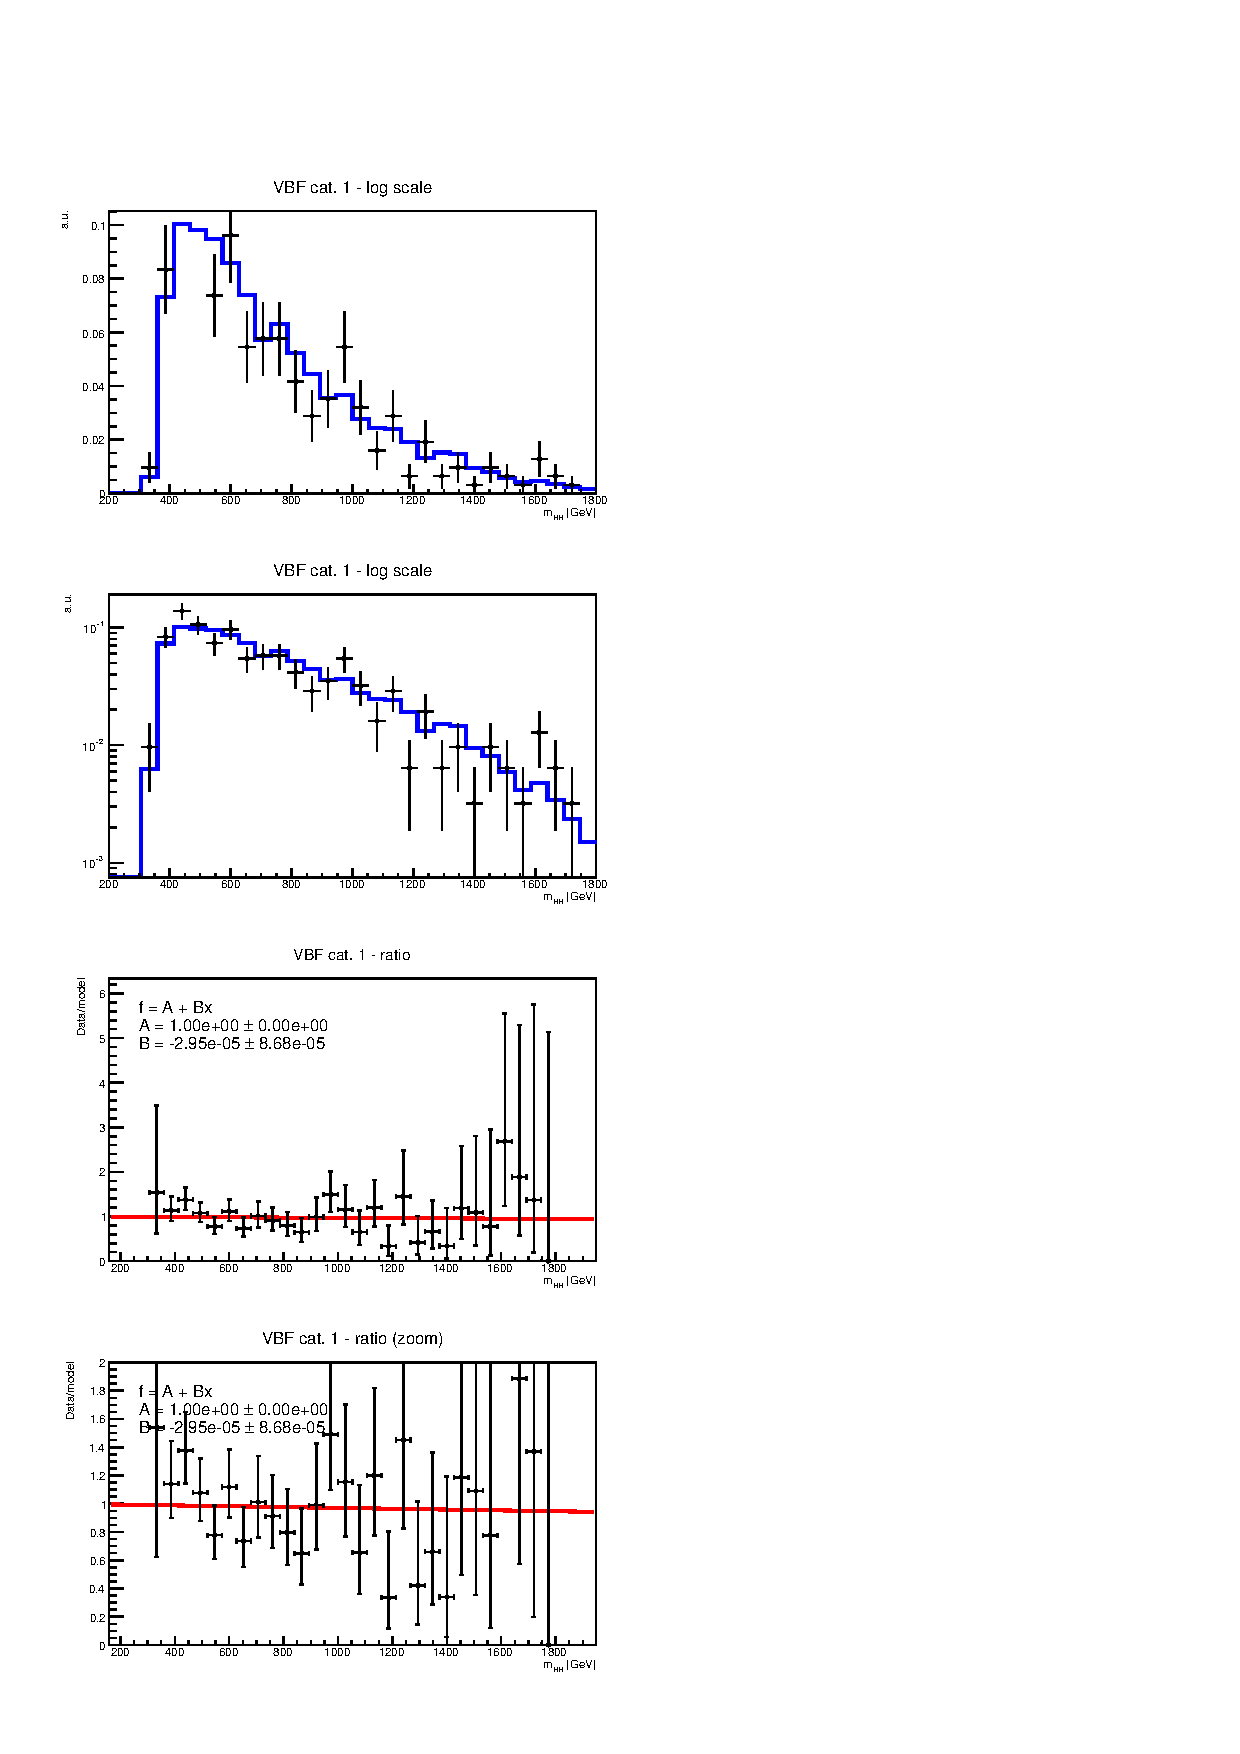
\includegraphics[width=0.32\textwidth,page=1]{Figures/Modeling/background/sketches/fixedA_overlay_2016_VBFcat1.pdf}}
\subfloat[]{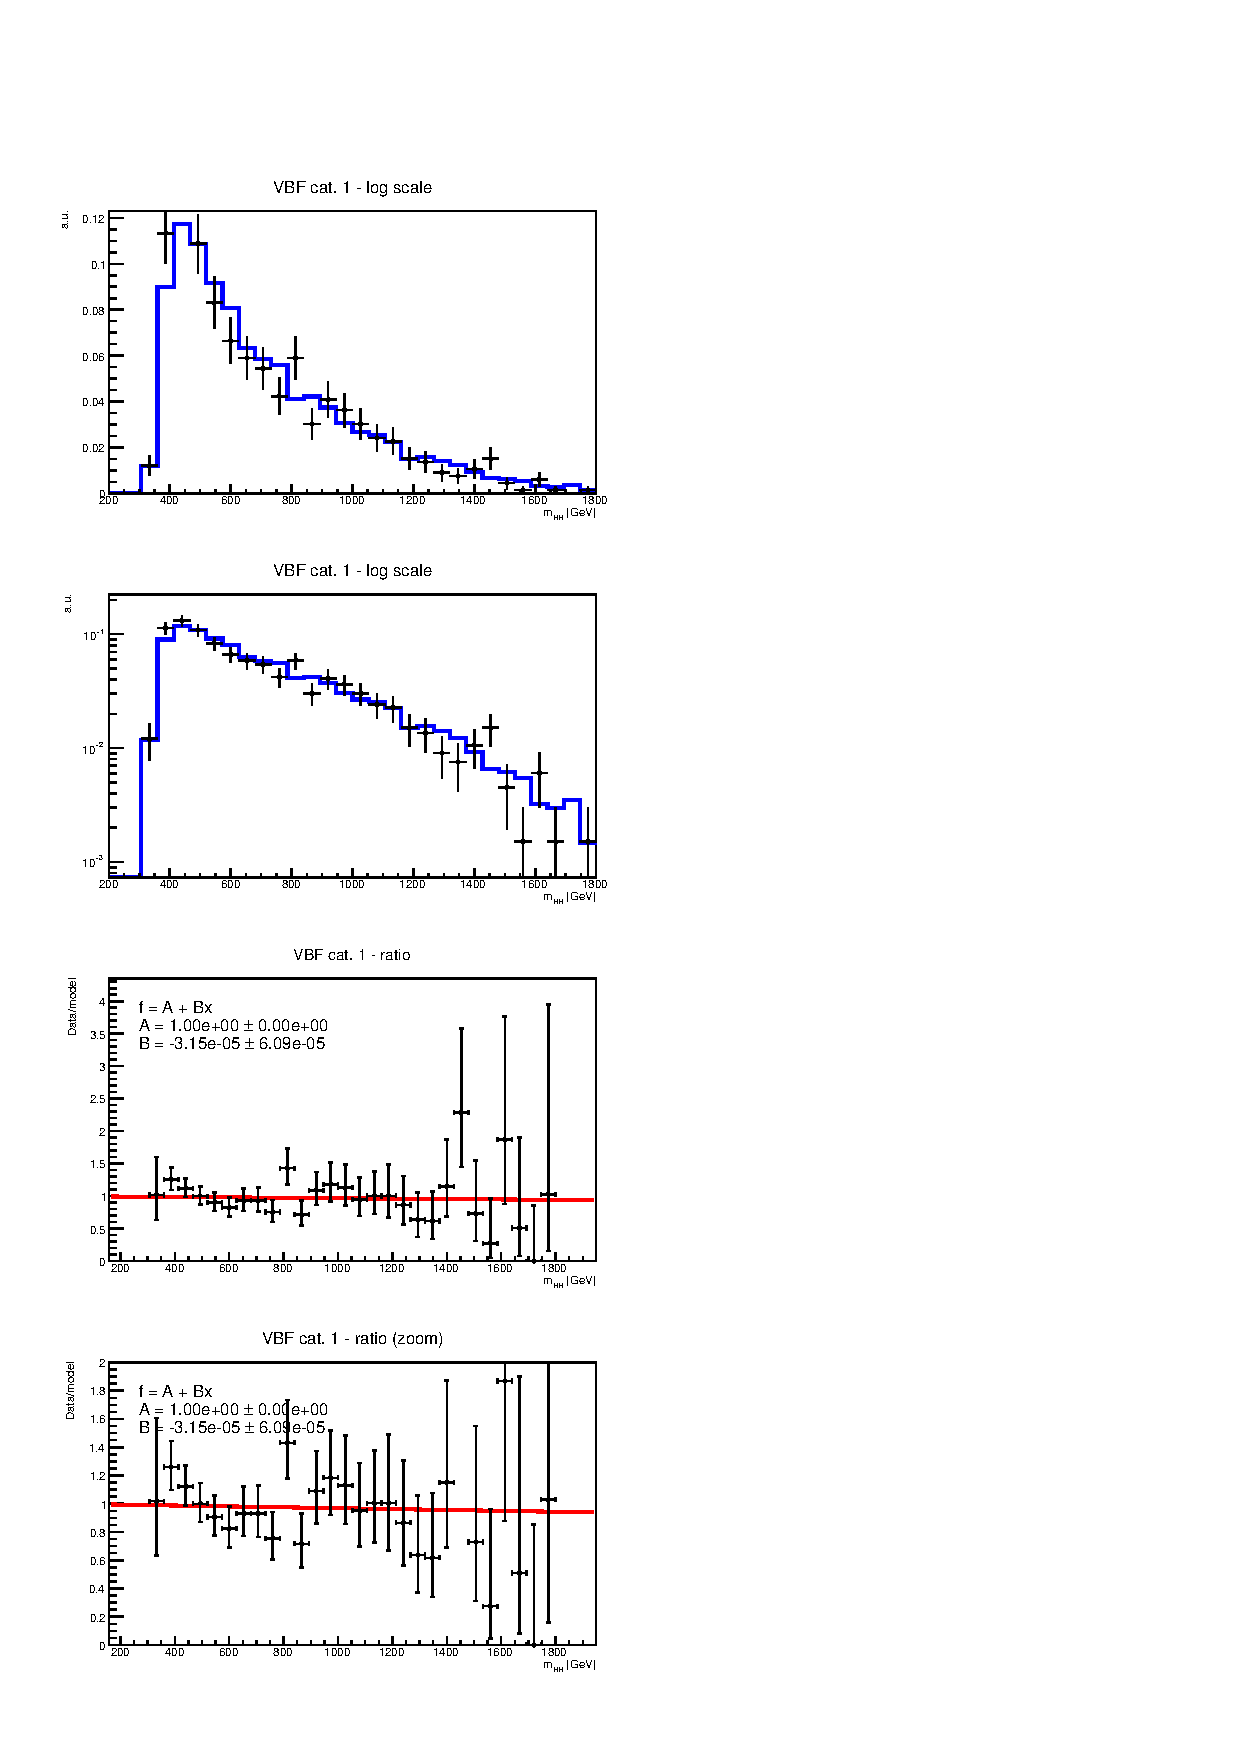
\includegraphics[width=0.32\textwidth,page=1]{Figures/Modeling/background/sketches/fixedA_overlay_20172018_VBFcat1.pdf}}
\caption[Linear fits used to derive a shape uncertainty for VBF category 1]{Linear fits used to derive a shape uncertainty for VBF category 1. A) 2016 fits and B) 2017-2018 fits.}
\label{fig:syst:VBFfits}
\end{figure}
\begin{figure}[ht!]
\centering
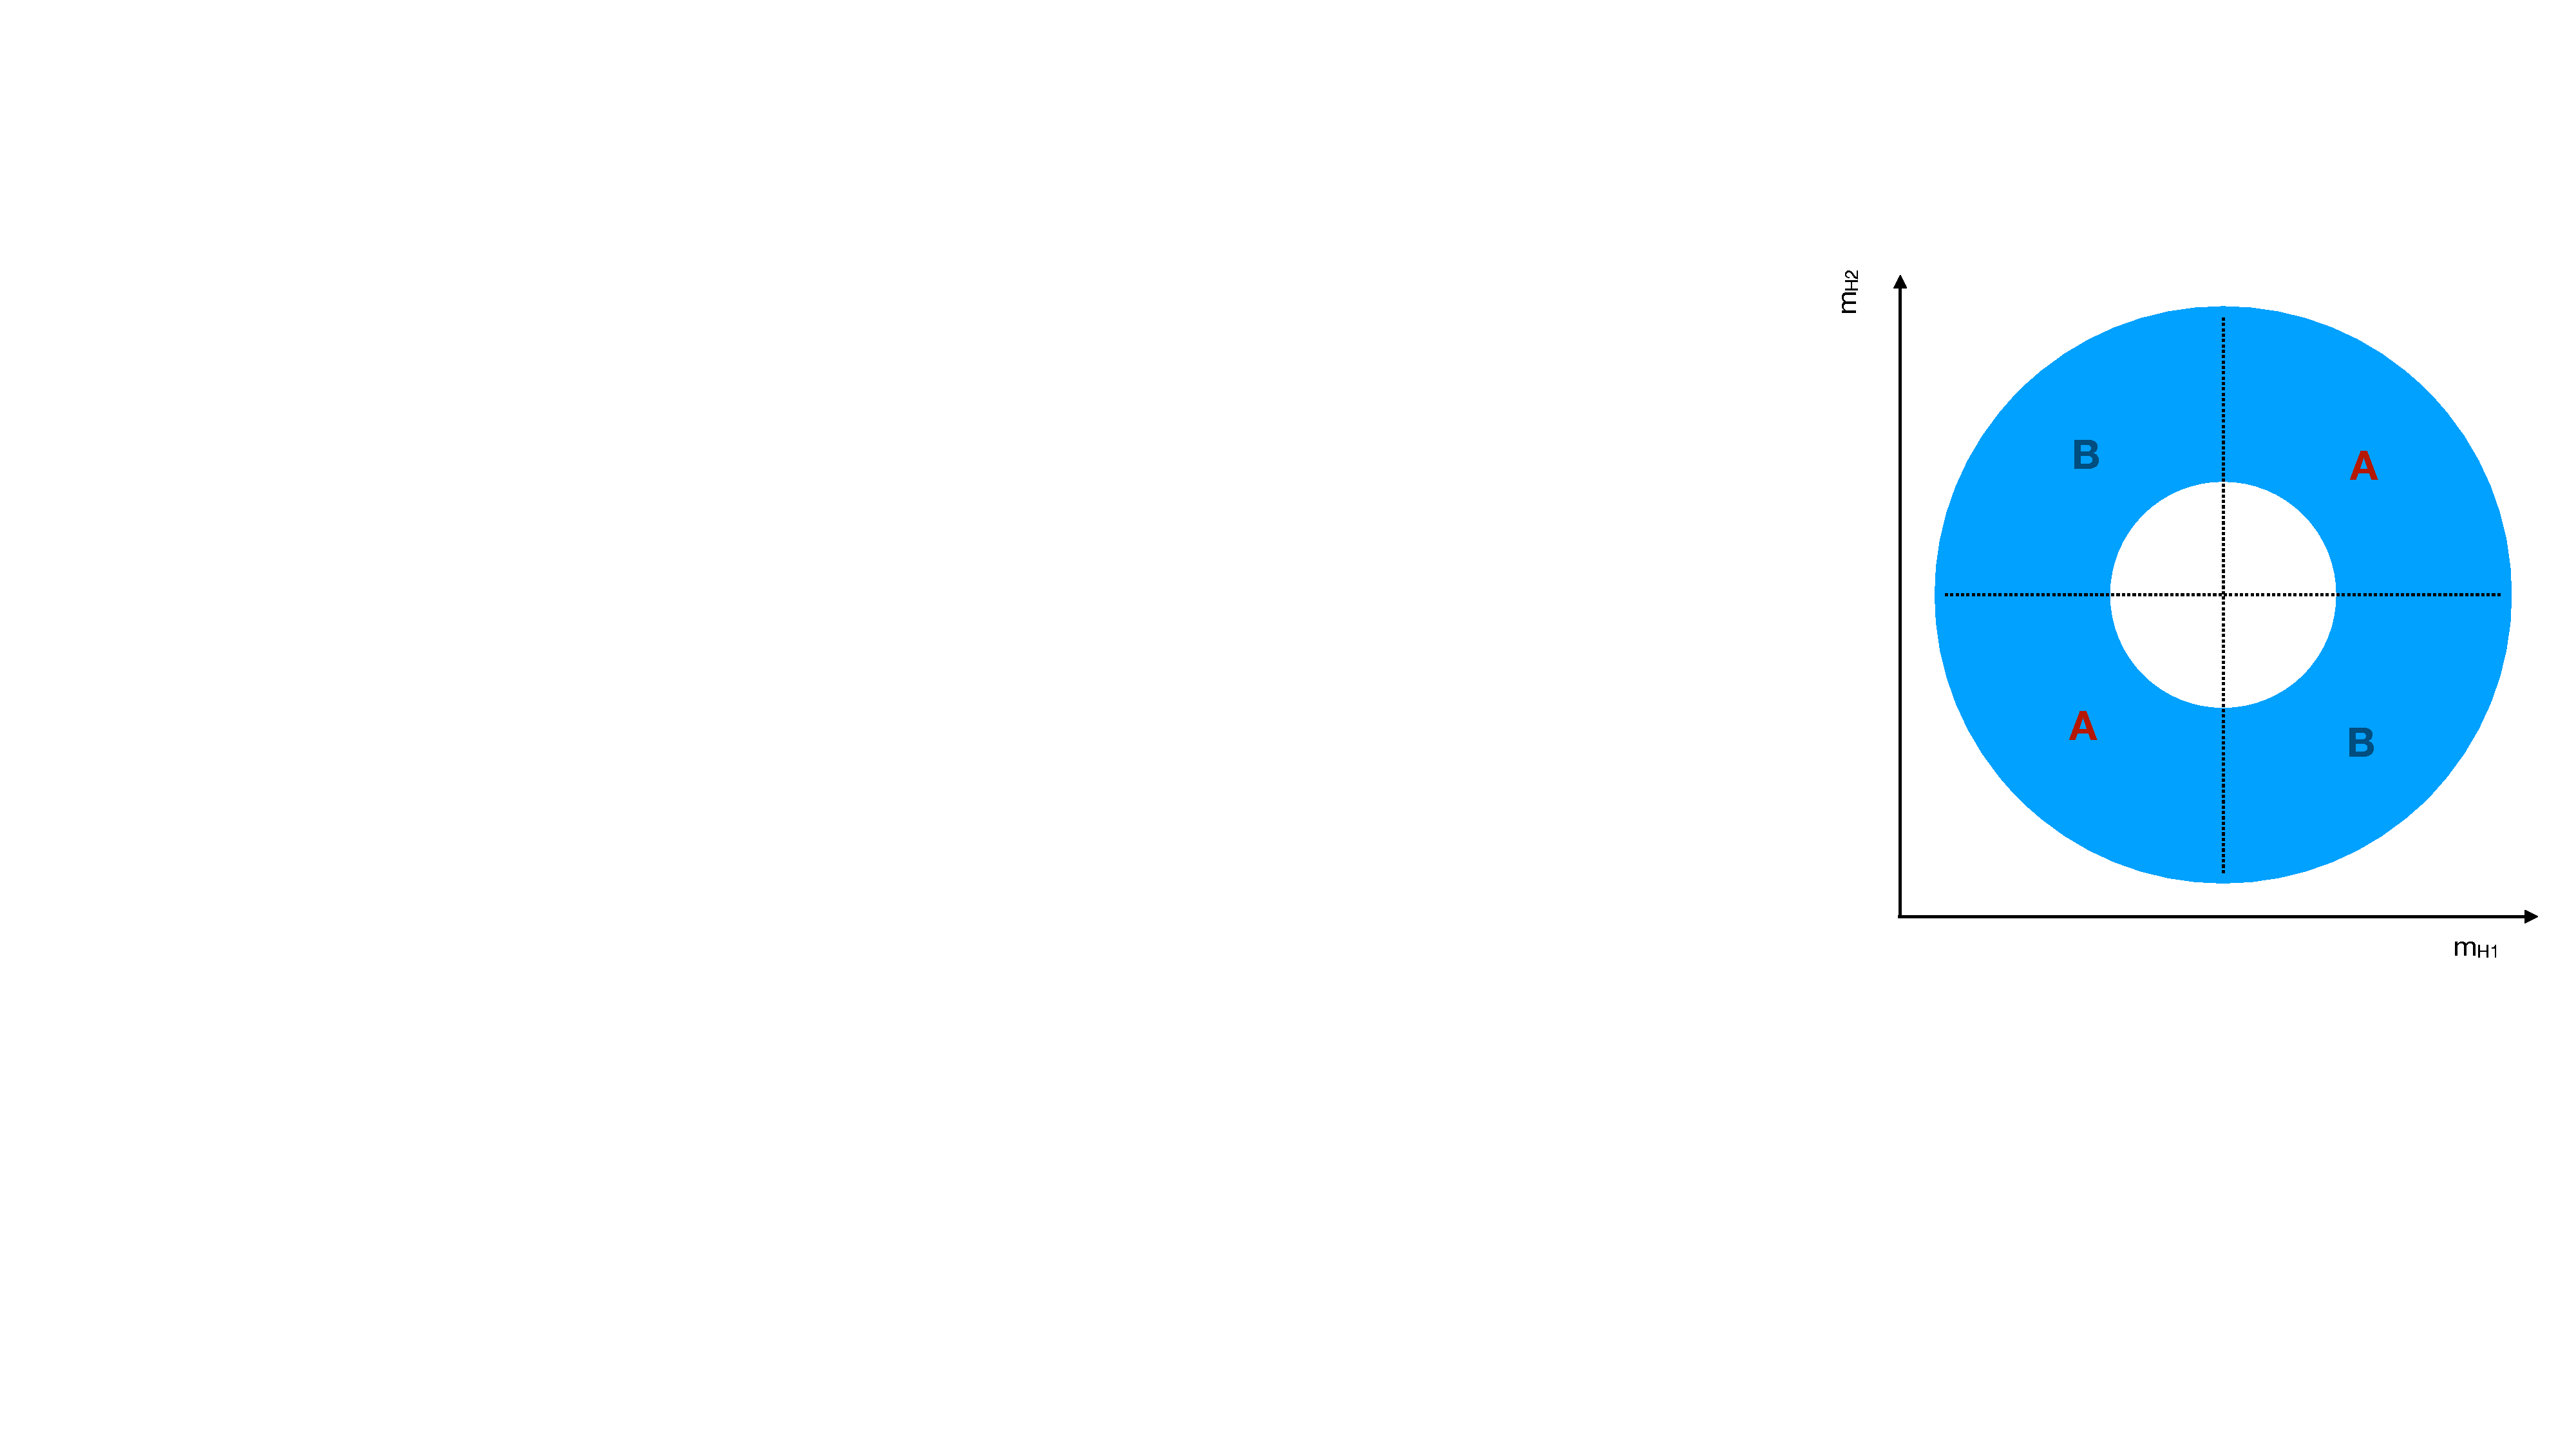
\includegraphics[width=0.25\textwidth,page=1]{Figures/Modeling/background/sketches/bkg_shape_unc_regions.pdf}
\caption[Regions used to determine the background shape uncertainty in ggF categories]{Regions used to determine the background shape uncertainty in ggF categories.}
\label{fig:syst:bkgshaperegions}
\end{figure}

\clearpage

\begin{table}[ht!]
\centering
\caption[Summary of the background model uncertainties in the 2016 analysis]{\label{syst:bkg2016}Summary of the background model uncertainties in the 2016 analysis.}
\begin{tabularx}{\textwidth}{l X X X X}
    \hline
    Uncertainty sources           & ggF Cat1 & ggF Cat 2 & VBF Cat1 &  VBF Cat 2\\   
    \hline
    Transfer factor (\%)          &  1.8     &      1.3  &  3.2     &    31.7   \\
    Validation normalization (\%) &  3.2     &       -   &   -      &     -     \\
    Validation precision (\%)     &  0.4     &       -   &  3.0     &   29.5    \\
    Bin-by-bin                    & $\surd$  &  $\surd$  & $\surd$  &  $\surd$  \\
    Shape                         & $\surd$  &  $\surd$  & $\surd$  &   -       \\
    \hline
\end{tabularx}
\end{table}

\begin{table}[ht!]
\caption[Summary of the background model uncertainties in the 2017-2018 analysis]{\label{syst:bkg20172018}Summary of the background model uncertainties in the 2017-2018 analysis.}
\centering
\begin{tabularx}{\textwidth}{l X X X X}
    \hline
    Uncertainty sources           & ggF Cat1 & ggF Cat 2 & VBF Cat1 &  VBF Cat 2\\   
    \hline
    Transfer factor (\%)          &  1.4     &      0.9  &  2.2     &    17.7   \\
    Validation normalization (\%) &  4.7     &      1.5  &   -      &     -     \\
    Validation precision (\%)     &   -      &      0.3  &  2.2     &   33.3    \\
    Bin-by-bin                    & $\surd$  &  $\surd$  & $\surd$  &  $\surd$  \\
    Shape                         & $\surd$  &  $\surd$  & $\surd$  &     -     \\
    \hline
\end{tabularx}
\end{table}

\subsection{Expected Impact of Nuisance Parameters} \label{syst:expectedimpacts}
The signal and background uncertainties of the analysis are defined as nuisance parameters $\theta$ in the statistical model further described in Section~\ref{results:statmodel}. The predicted or `pre-fit' nuisance parameter have a default value ($\theta_{0}$) and $\pm1$ standard deviation uncertainties ($\Delta_{\theta}$). The presence of a signal can be determined by measuring the best-fit to the signal strength ($\hat{\mu}$). The signal strength $\mu$ is the parameter used to scale the signal cross section with respect to the values used for the signal normalization. The measurement of $\hat{\mu}$ is carried out by a maximum likelihood fit of the signal plus background ($\mu s+b$) model to the observed data, in which the nuisance parameters are floated. The corresponding fitted or `post-fit' value and uncertainty of the nuisance parameters are denoted as $\hat{\theta}$ and $\Delta$, respectively. 

To understand the importance or `impact' of a systematic uncertainty in the statistical analysis, the procedure is to determine how the corresponding nuisance parameter $\theta$ affects the measurement of $\hat{\mu}$. Then, one evaluates the shift $\Delta\hat{\mu}$ induced when the nuisance parameter is set at its $\pm1$ post-fit values. Large $\Delta\hat{\mu}$ values imply a strong dependency of the signal strength on that systematic uncertainty. Moreover, one can compare the pre-fit and post-fit nominal value by computing the pull defined as ($\hat{\theta}-\theta_{0}$)/$\Delta_{0}$. The pull error bars are defined as the ratio between $\Delta$ and $\Delta_{0}$. If they are smaller than 1, the nuisance parameter uncertainties are constrained in the fit. 

Before the looking at the data, the blinded procedure is to compute the expected nuisance parameter impacts. They are evaluated using the `Asimov' dataset,  i.e. the prediction at the median expected from the $\mu s+b$ model. Moreover, the nuisance parameters and signal strength are set to their pre-fit values. As the HH signal is not observed yet at the LHC, $\mu$ is set at 7.3, which is the expected 95 \% CL upper limit on $\mu$ using all Run-2 categories. This blinded limit is obtained using the method described in Subsection~\ref{results:statmodel} based on the a-priori background distribution instead of the observed data. The nuisance parameters with the largest expected impact are presented in Figure~\ref{fig:syst:expectedimpacts}. The behavior of the systematic uncertainties is as expected. They show that the background model uncertainties are the dominant uncertainties in this search. In particular, the background uncertainties associated to the ggF category 2 have the most impact. The largest impact of a signal uncertainty comes from the trigger measurement.

\begin{figure}[ht!]
\centering
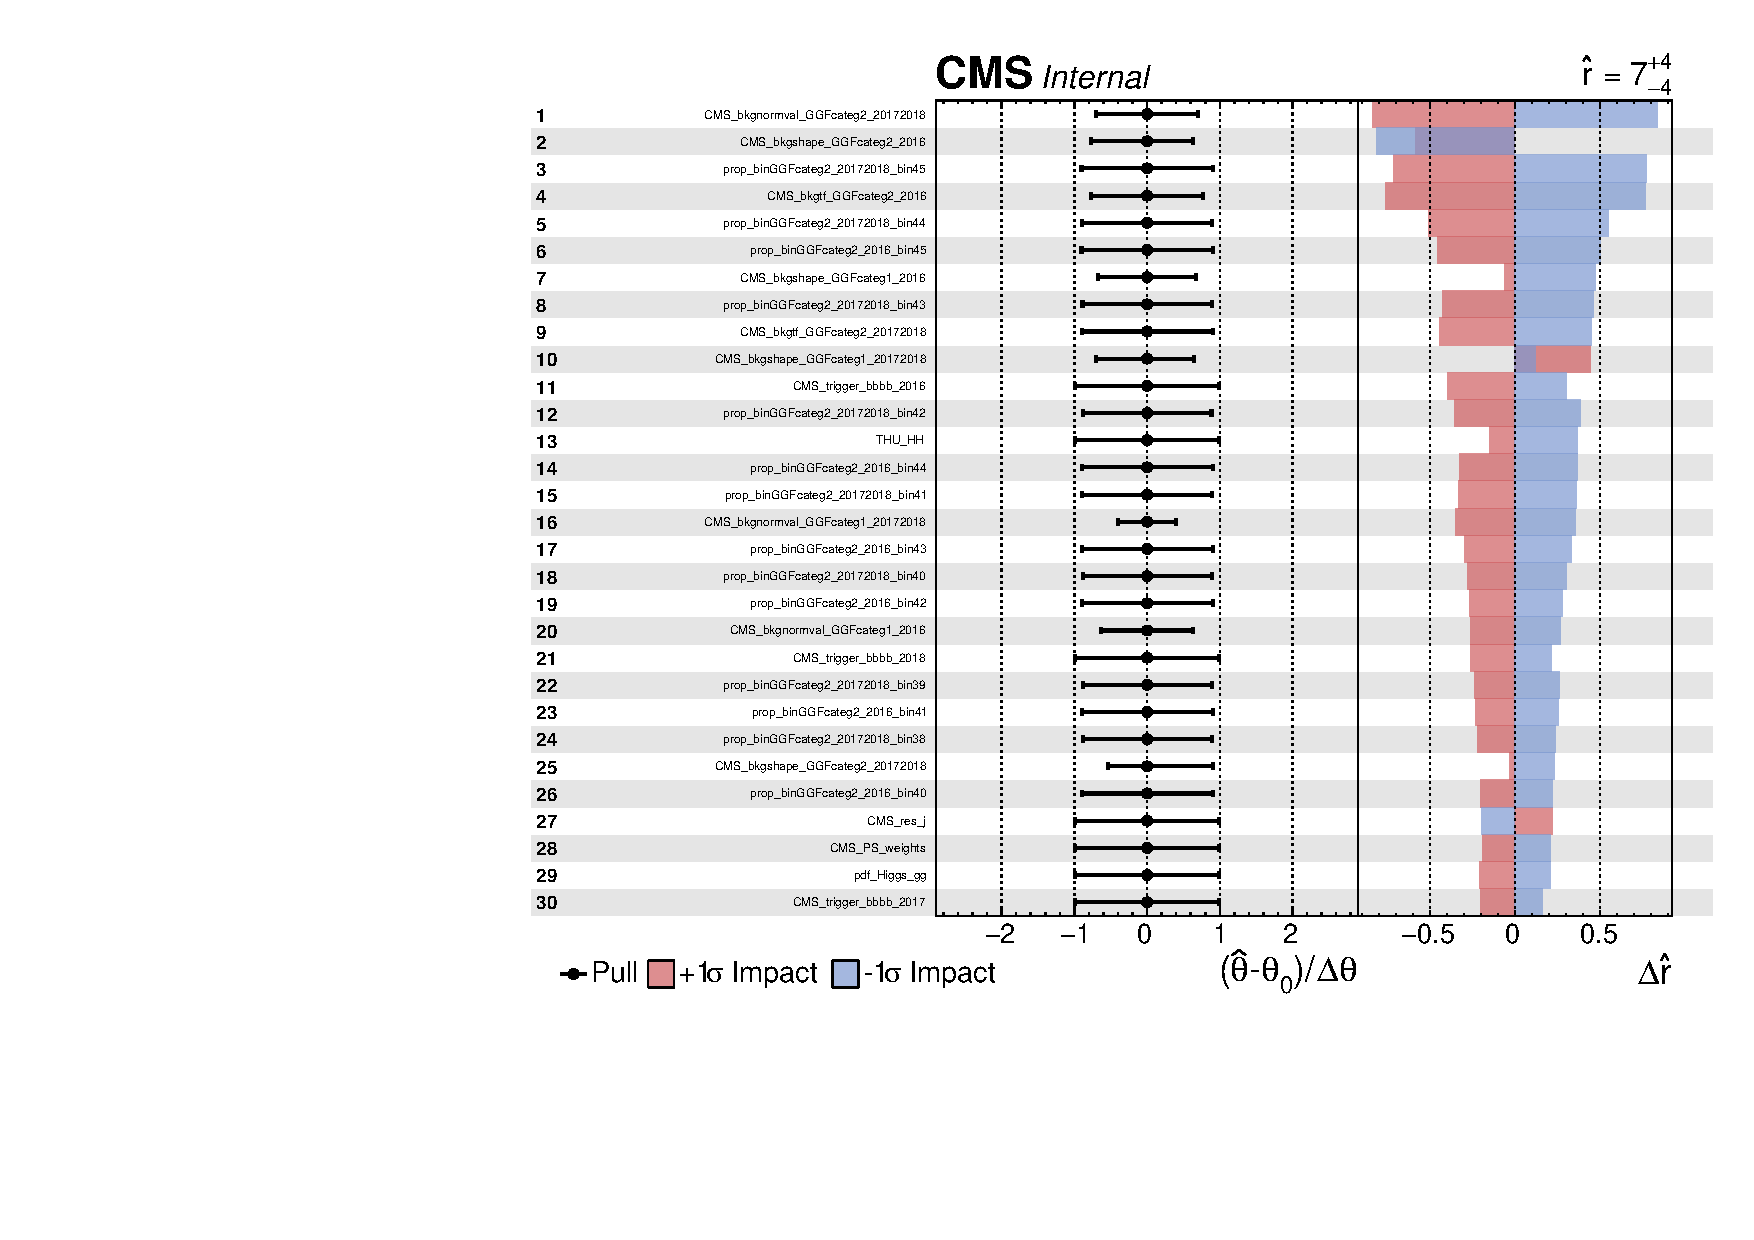
\includegraphics[width=0.82\textwidth,page=1]{Figures/Results/systematics/impacts_sig_inj7p2_expected.pdf}
\caption[Expected impact of the highest systematic uncertainties on the measurement of the signal strength]{Expected impact of the highest systematic uncertainties on the measurement of the signal strength ($\hat{r}$) using all Run-2 categories.}
\label{fig:syst:expectedimpacts}
\end{figure}